\newpage
\clearpage
\vspace*{\fill}
% \chapter{Sample and distribution details}
\section{$\mtas$ distributions, boosted $W/Z$}
\vfill
\clearpage
\twocolumn

\begin{figure}
 
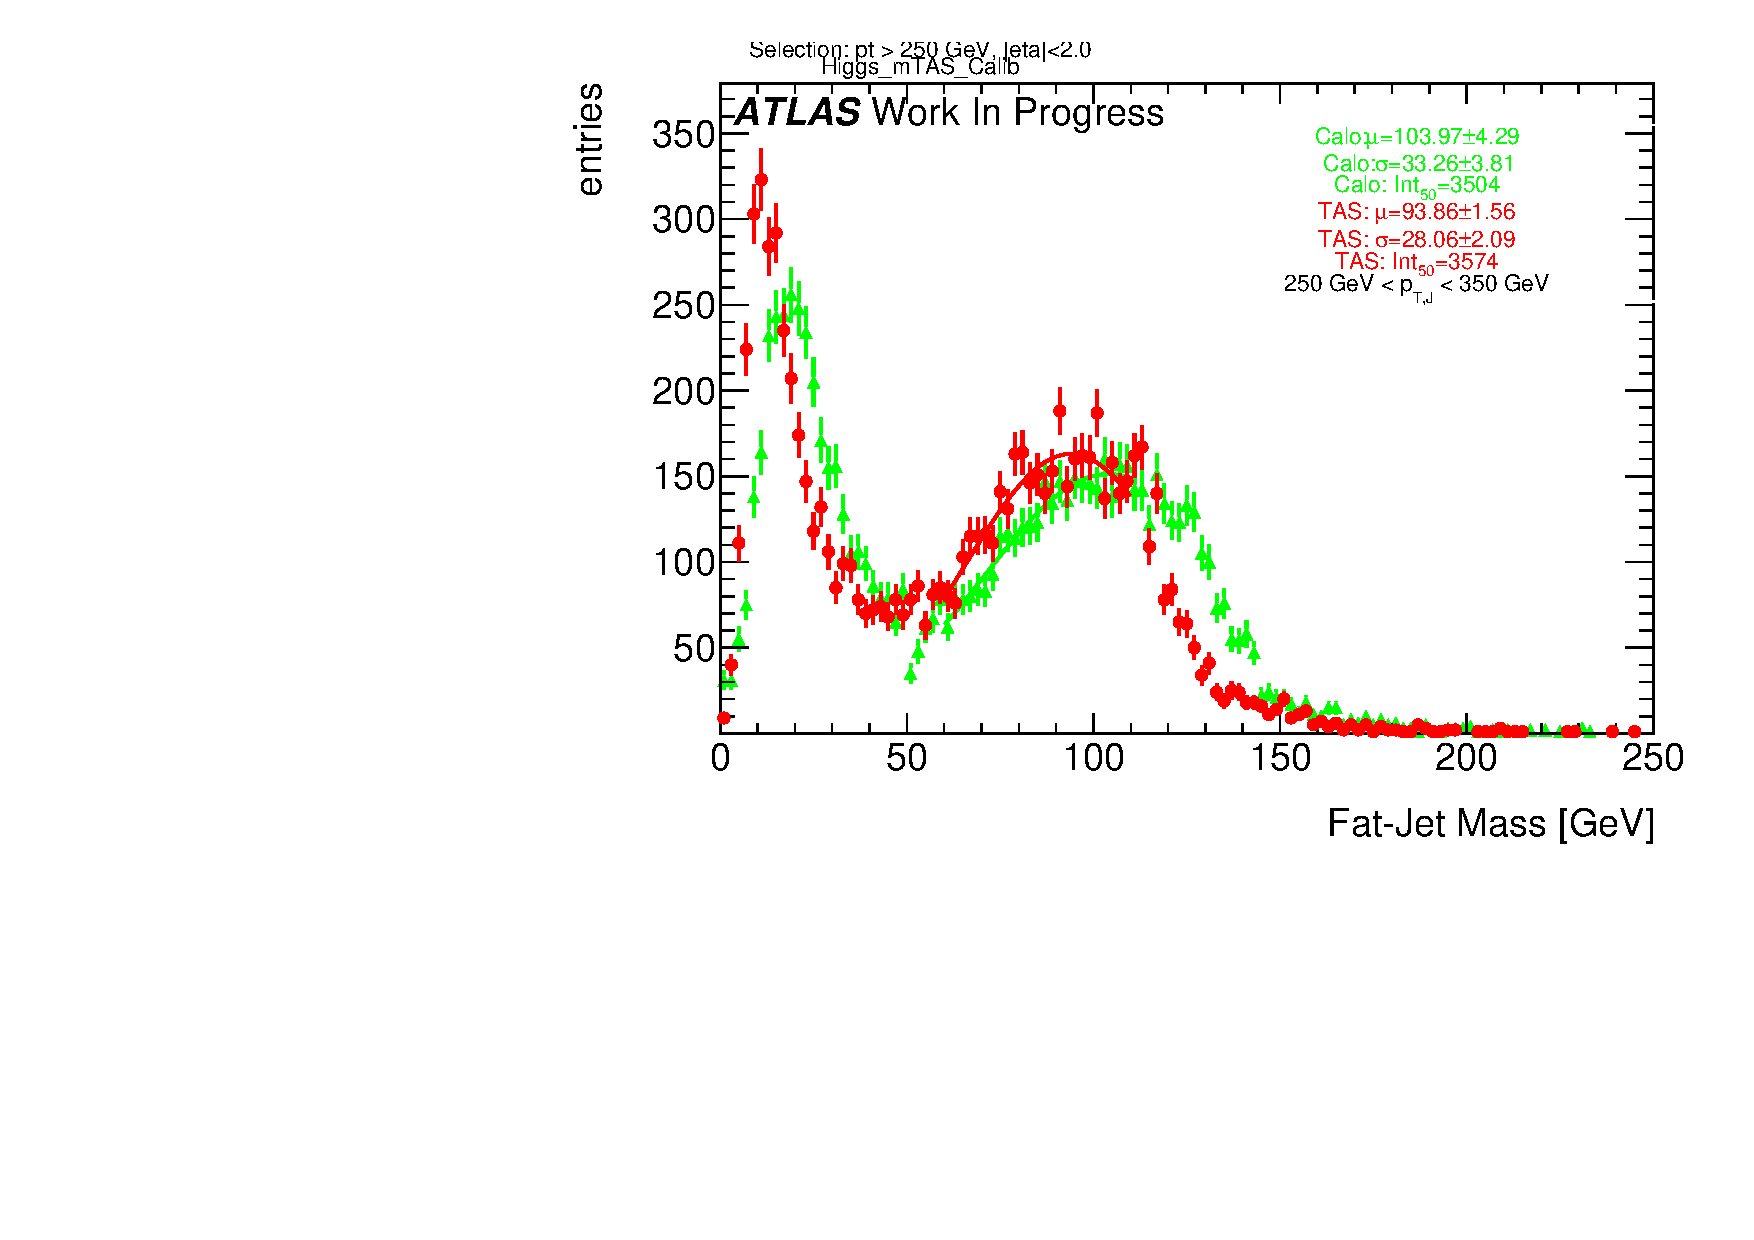
\includegraphics[width=0.4\textwidth]{/Users/fabnap/Documents/MasterArbeit/appendixB/mTAS_W_calibmCal_20:07:01-03-11-2016/12cfrt_h_FatJet_ptJ01m.pdf}
\caption{$\mtas$ and $\mcal$ for $p_{T}^{J}$ bin (indicated on plot) }
 
\end{figure}
 
\begin{figure}
 
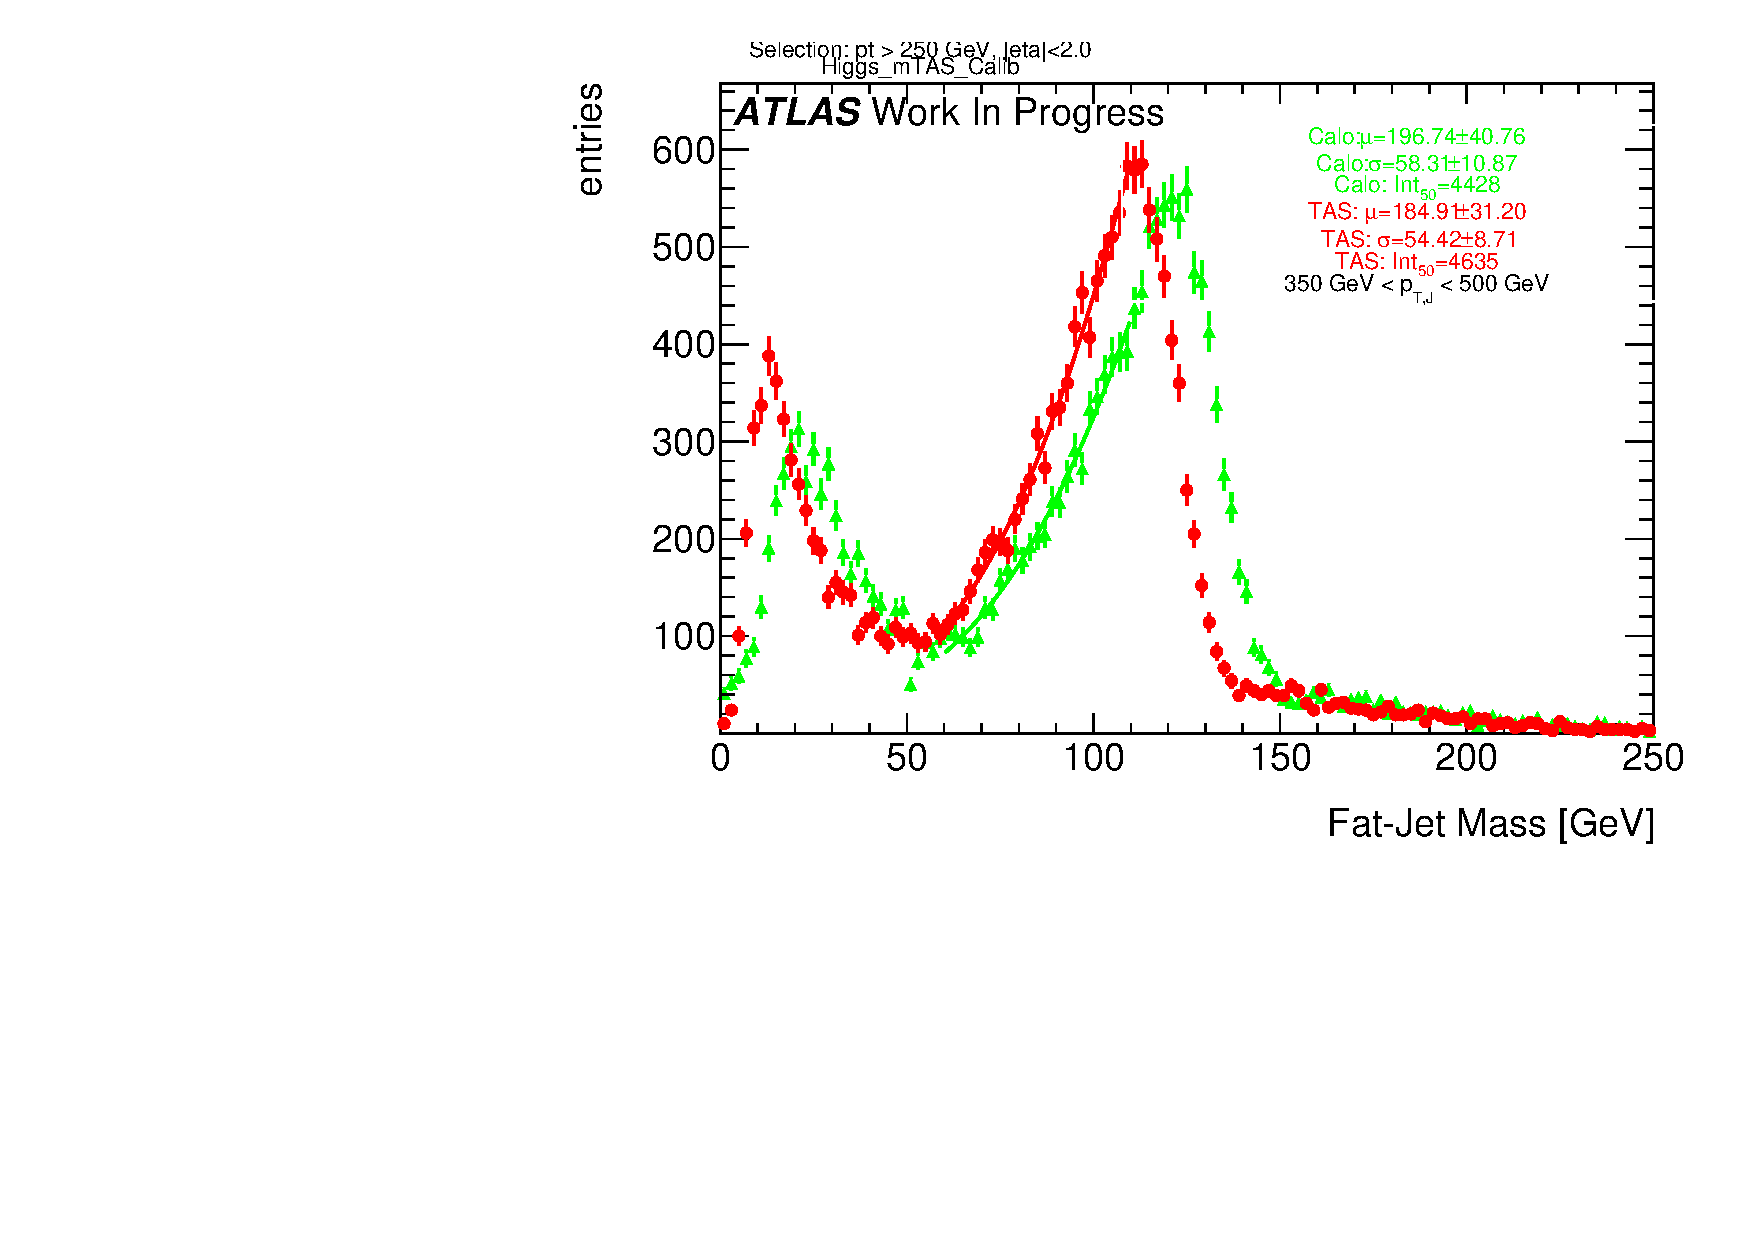
\includegraphics[width=0.4\textwidth]{/Users/fabnap/Documents/MasterArbeit/appendixB/mTAS_W_calibmCal_20:07:01-03-11-2016/12cfrt_h_FatJet_ptJ02m.pdf}
\caption{$\mtas$ and $\mcal$ for $p_{T}^{J}$ bin (indicated on plot) }
 
\end{figure}
 
\begin{figure}
 
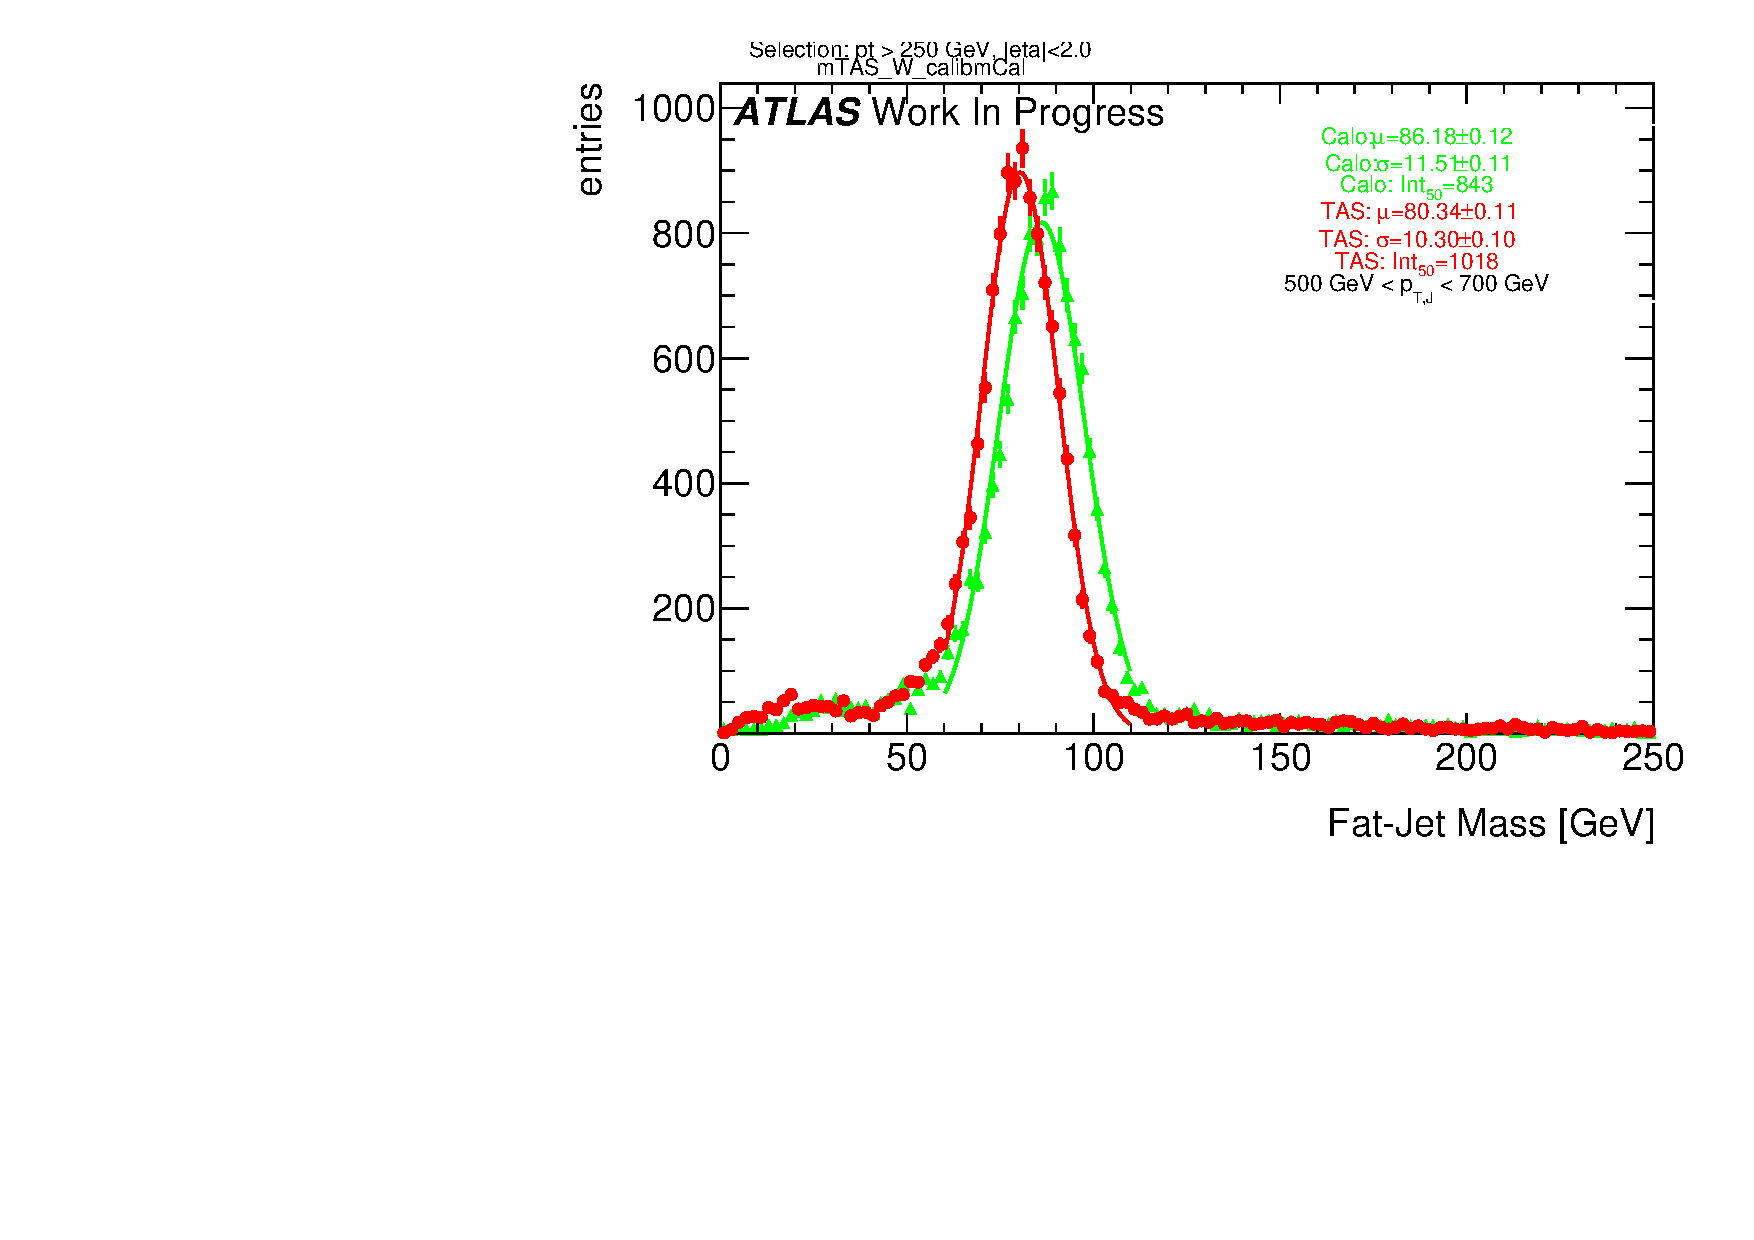
\includegraphics[width=0.4\textwidth]{/Users/fabnap/Documents/MasterArbeit/appendixB/mTAS_W_calibmCal_20:07:01-03-11-2016/12cfrt_h_FatJet_ptJ03m.pdf}
\caption{$\mtas$ and $\mcal$ for $p_{T}^{J}$ bin (indicated on plot) }
 
\end{figure}
 
\begin{figure}
 
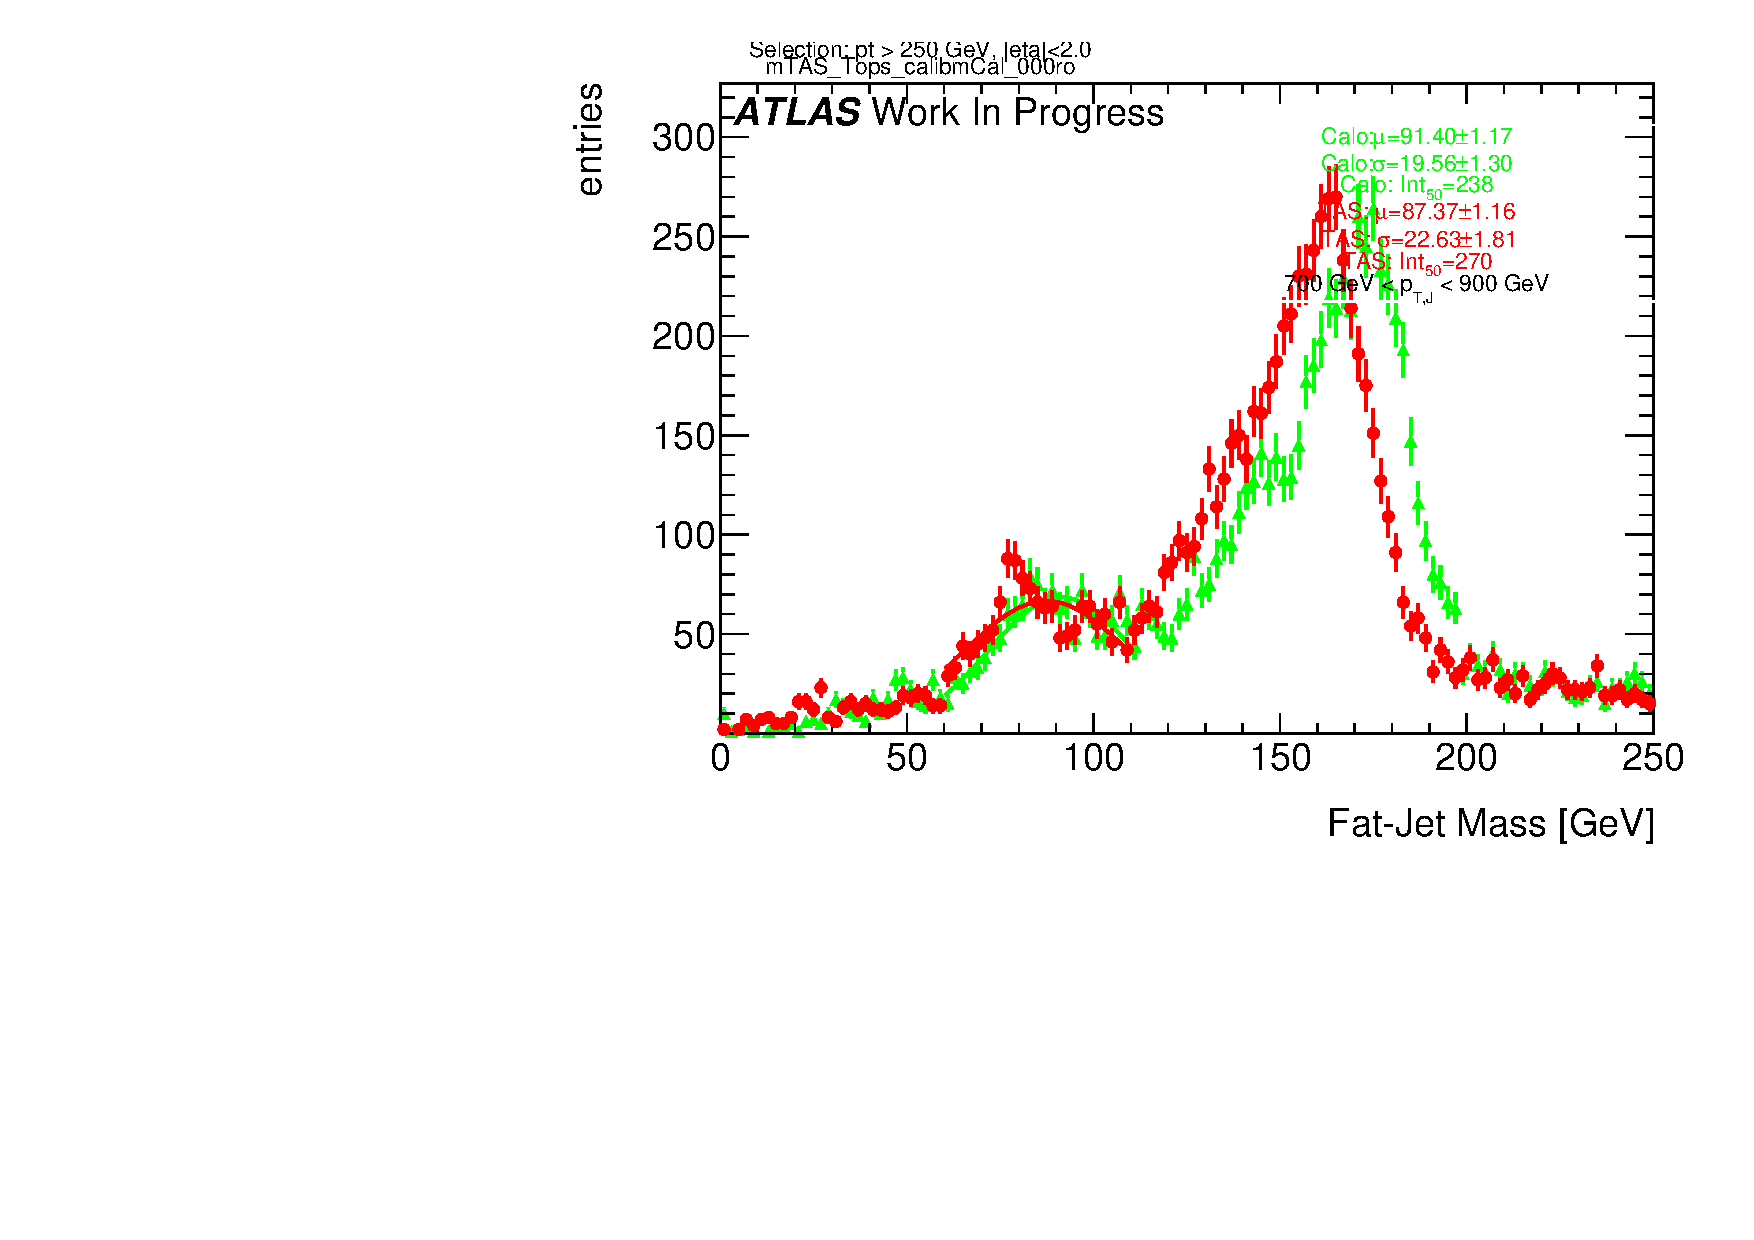
\includegraphics[width=0.4\textwidth]{/Users/fabnap/Documents/MasterArbeit/appendixB/mTAS_W_calibmCal_20:07:01-03-11-2016/12cfrt_h_FatJet_ptJ04m.pdf}
\caption{$\mtas$ and $\mcal$ for $p_{T}^{J}$ bin (indicated on plot) }
 
\end{figure}
 
\begin{figure}
 
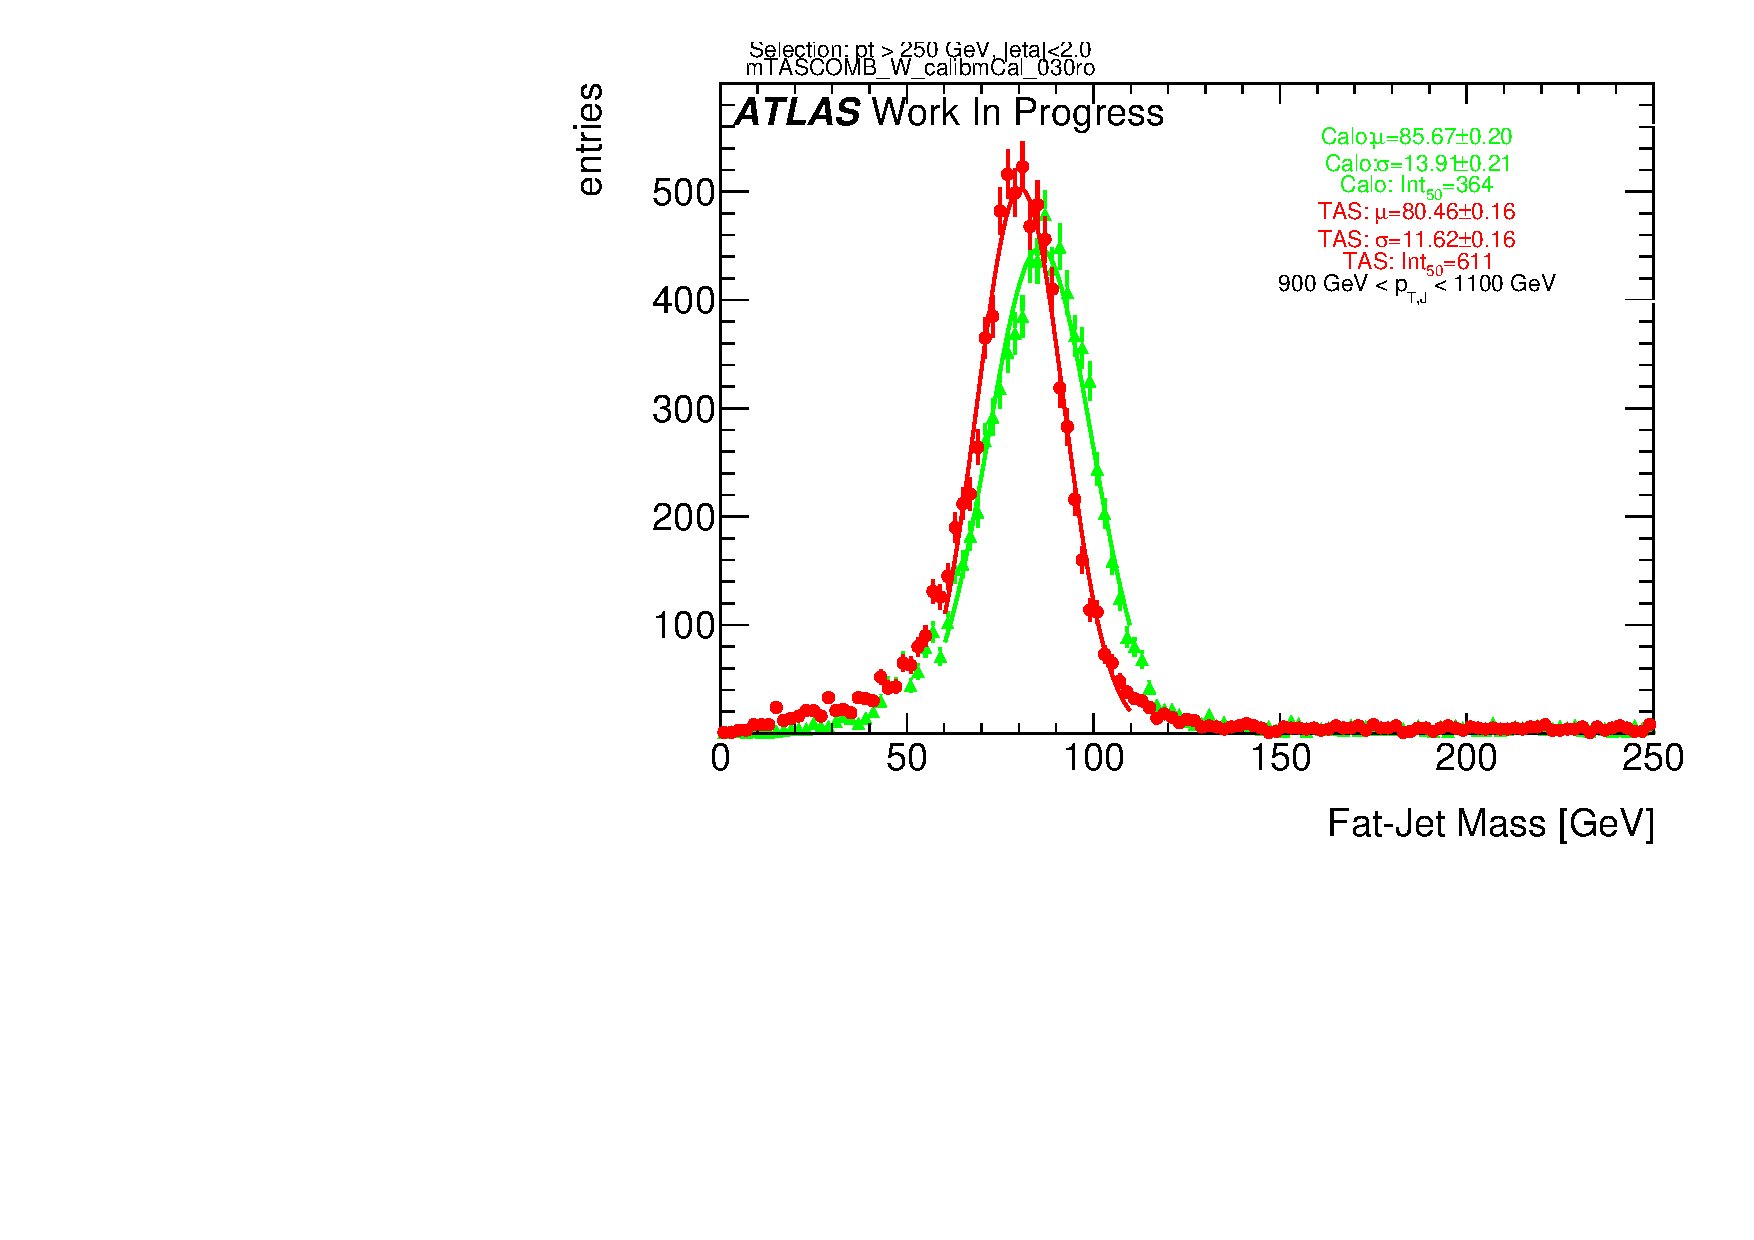
\includegraphics[width=0.4\textwidth]{/Users/fabnap/Documents/MasterArbeit/appendixB/mTAS_W_calibmCal_20:07:01-03-11-2016/12cfrt_h_FatJet_ptJ05m.pdf}
\caption{$\mtas$ and $\mcal$ for $p_{T}^{J}$ bin (indicated on plot) }
 
\end{figure}
 
\begin{figure}
 
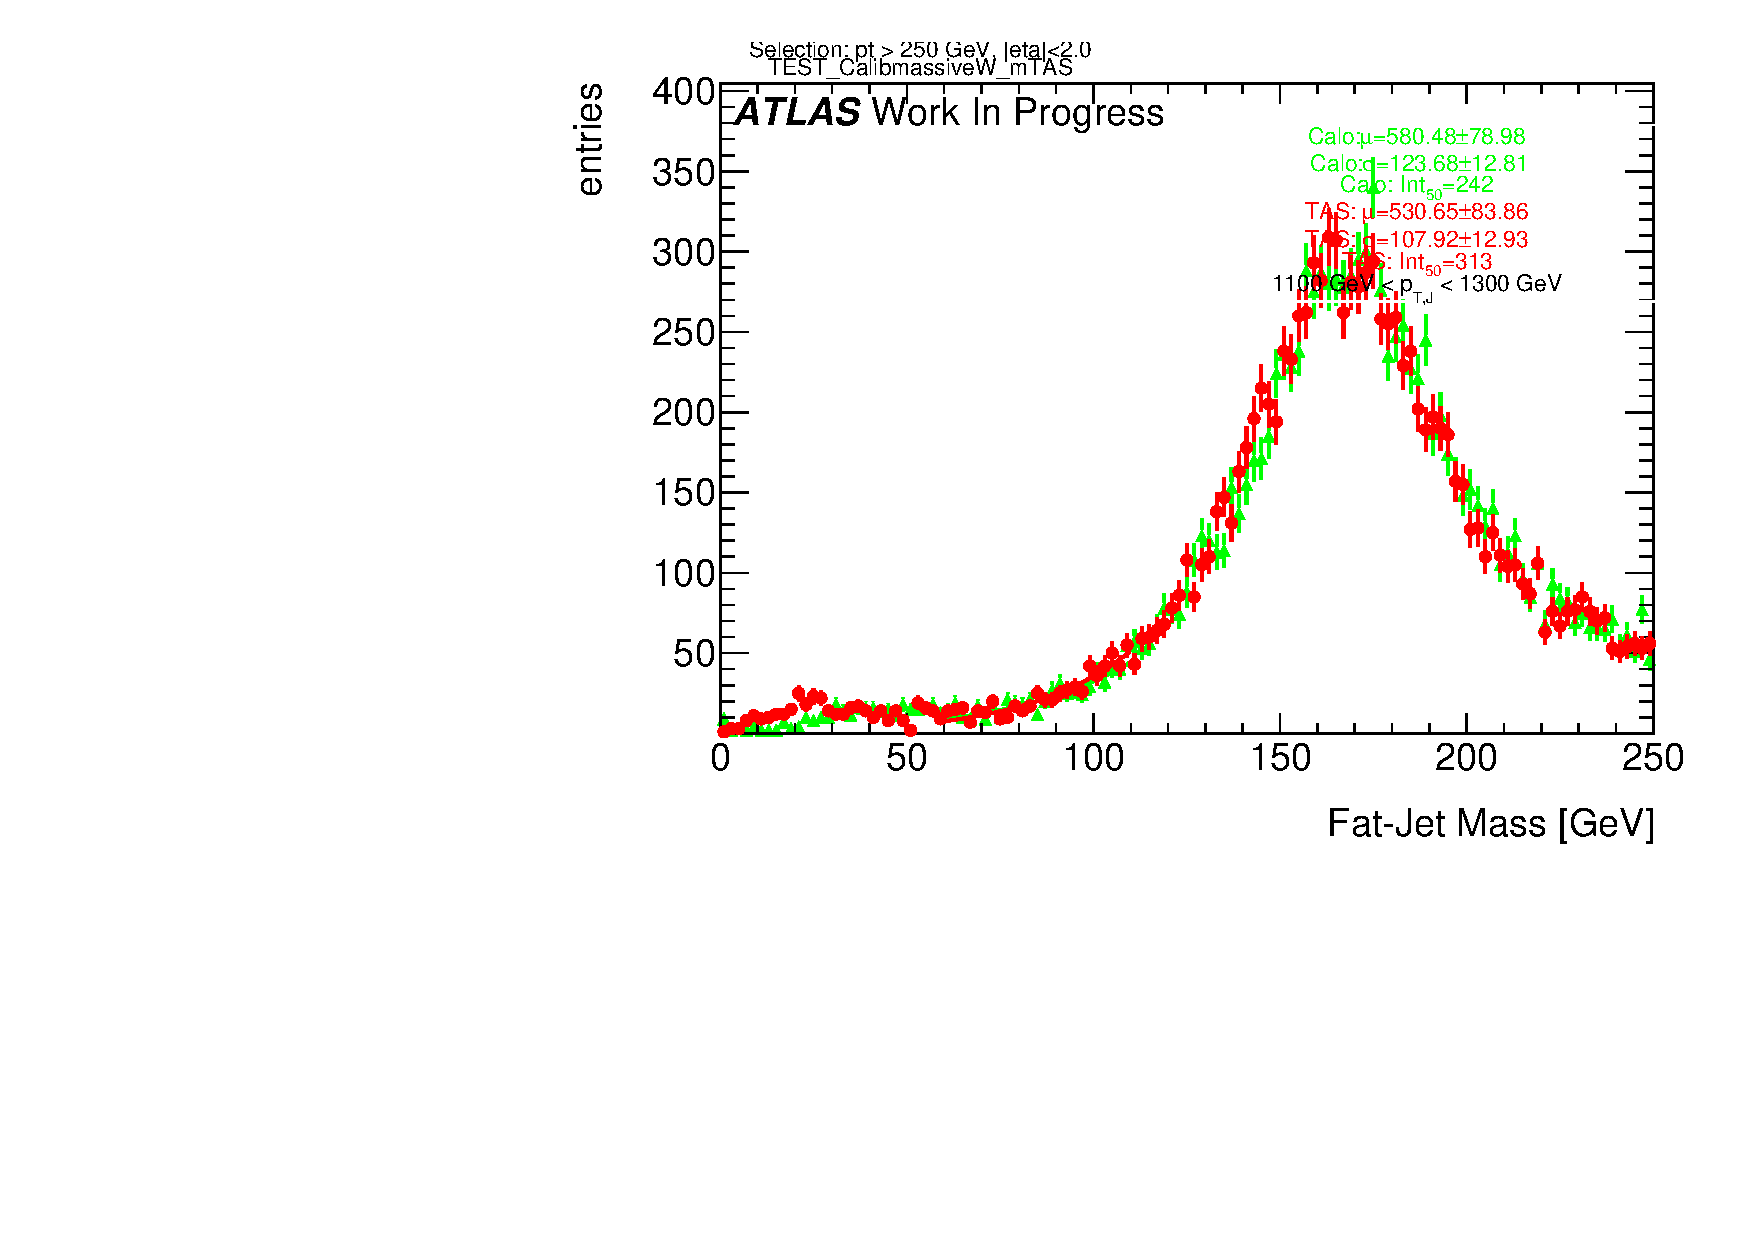
\includegraphics[width=0.4\textwidth]{/Users/fabnap/Documents/MasterArbeit/appendixB/mTAS_W_calibmCal_20:07:01-03-11-2016/12cfrt_h_FatJet_ptJ06m.pdf}
\caption{$\mtas$ and $\mcal$ for $p_{T}^{J}$ bin (indicated on plot) }
 
\end{figure}
 %
\begin{figure}
 
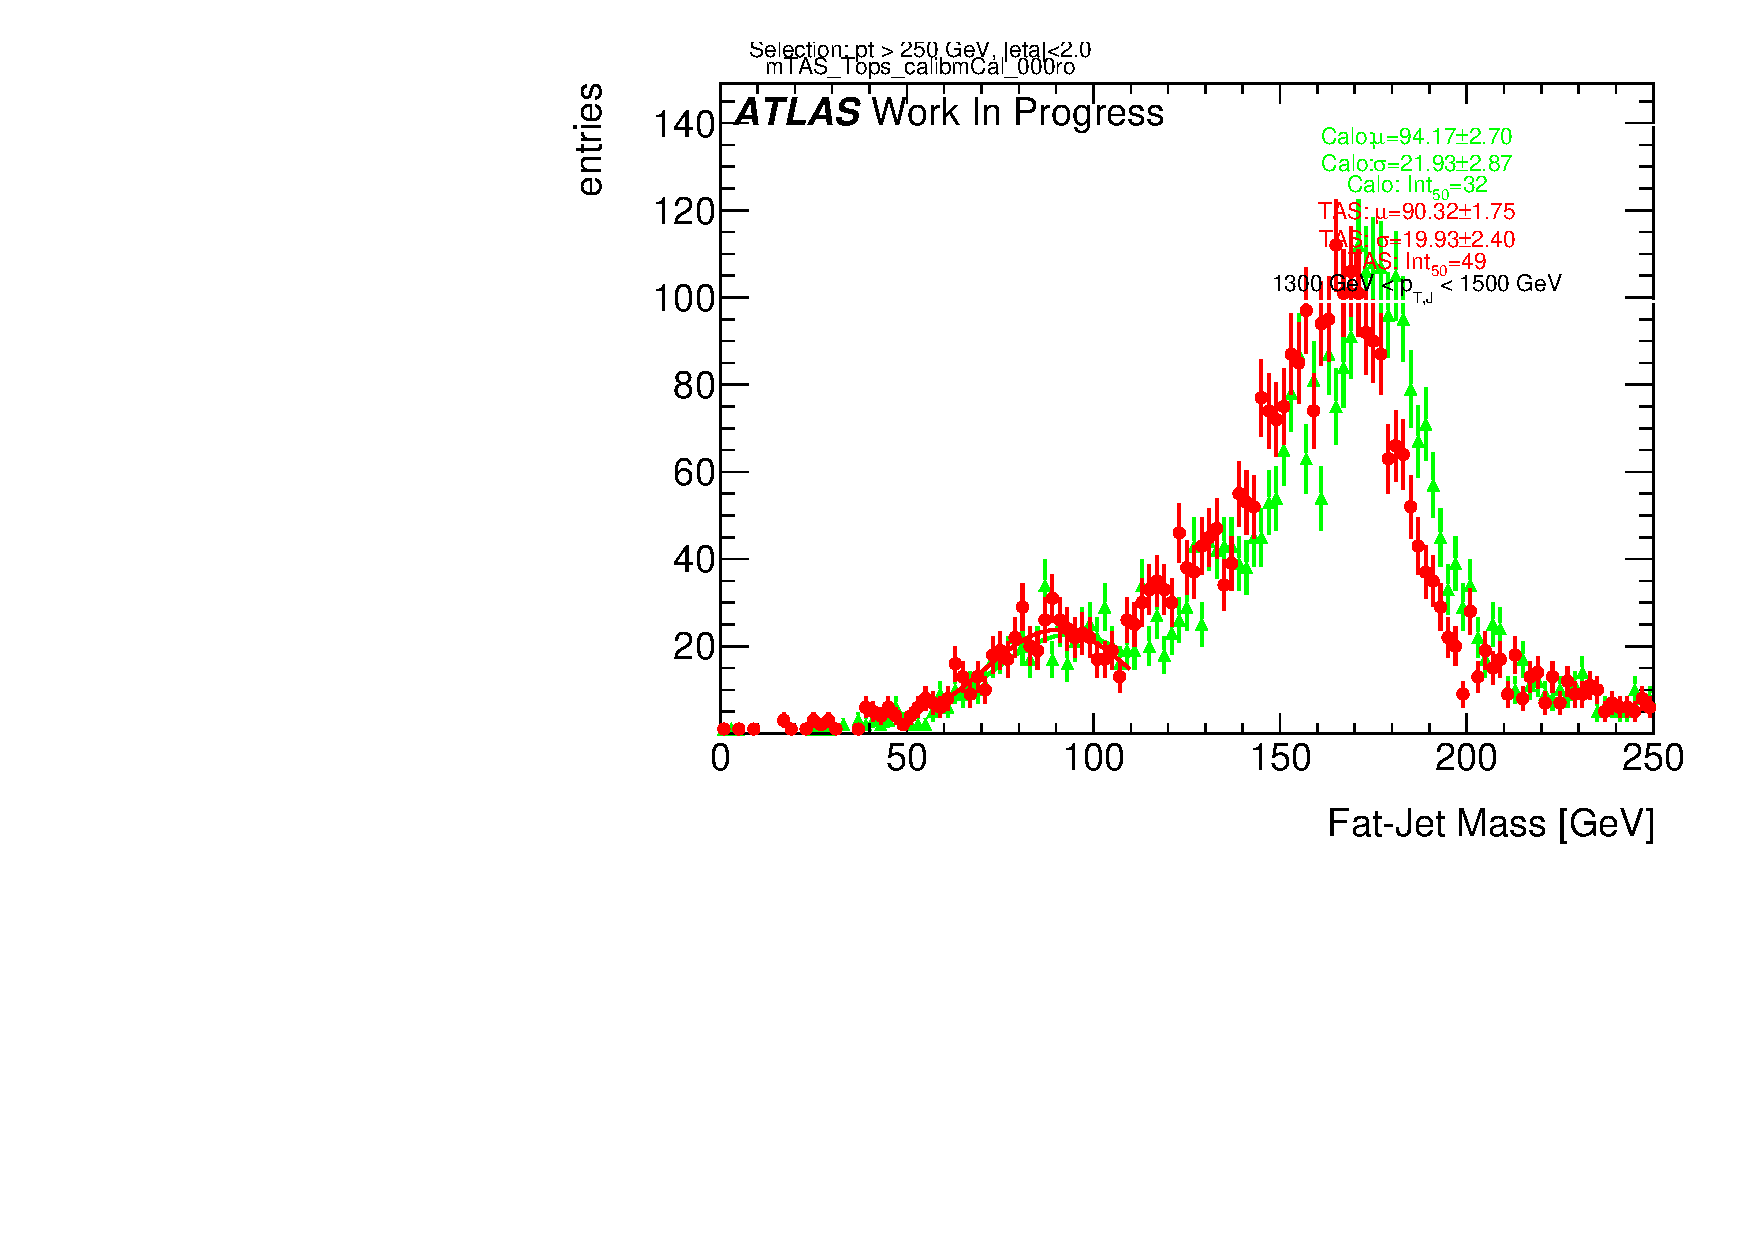
\includegraphics[width=0.4\textwidth]{/Users/fabnap/Documents/MasterArbeit/appendixB/mTAS_W_calibmCal_20:07:01-03-11-2016/12cfrt_h_FatJet_ptJ07m.pdf}
\caption{$\mtas$ and $\mcal$ for $p_{T}^{J}$ bin (indicated on plot) }
 
\end{figure}
 
\begin{figure}
 
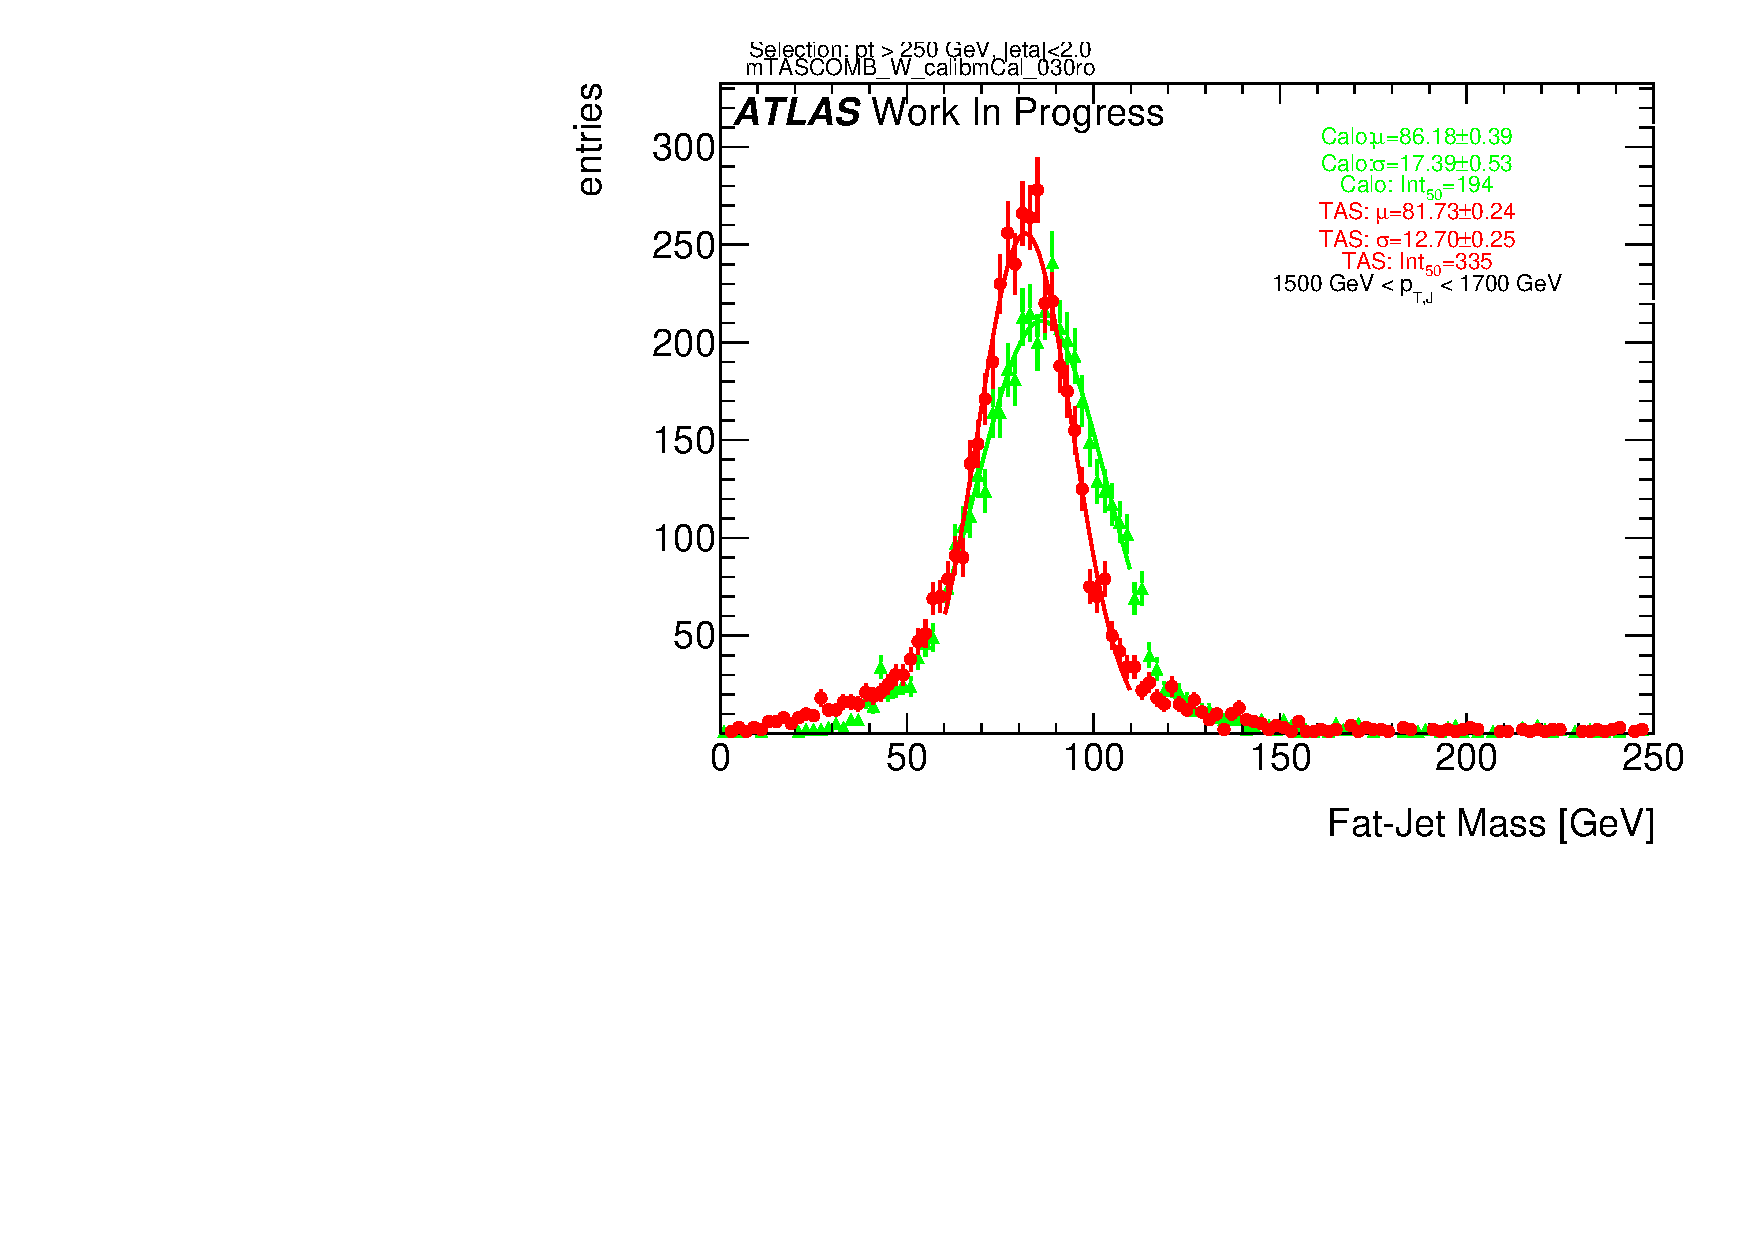
\includegraphics[width=0.4\textwidth]{/Users/fabnap/Documents/MasterArbeit/appendixB/mTAS_W_calibmCal_20:07:01-03-11-2016/12cfrt_h_FatJet_ptJ08m.pdf}
\caption{$\mtas$ and $\mcal$ for $p_{T}^{J}$ bin (indicated on plot) }
 
\end{figure}
 
\begin{figure}
 
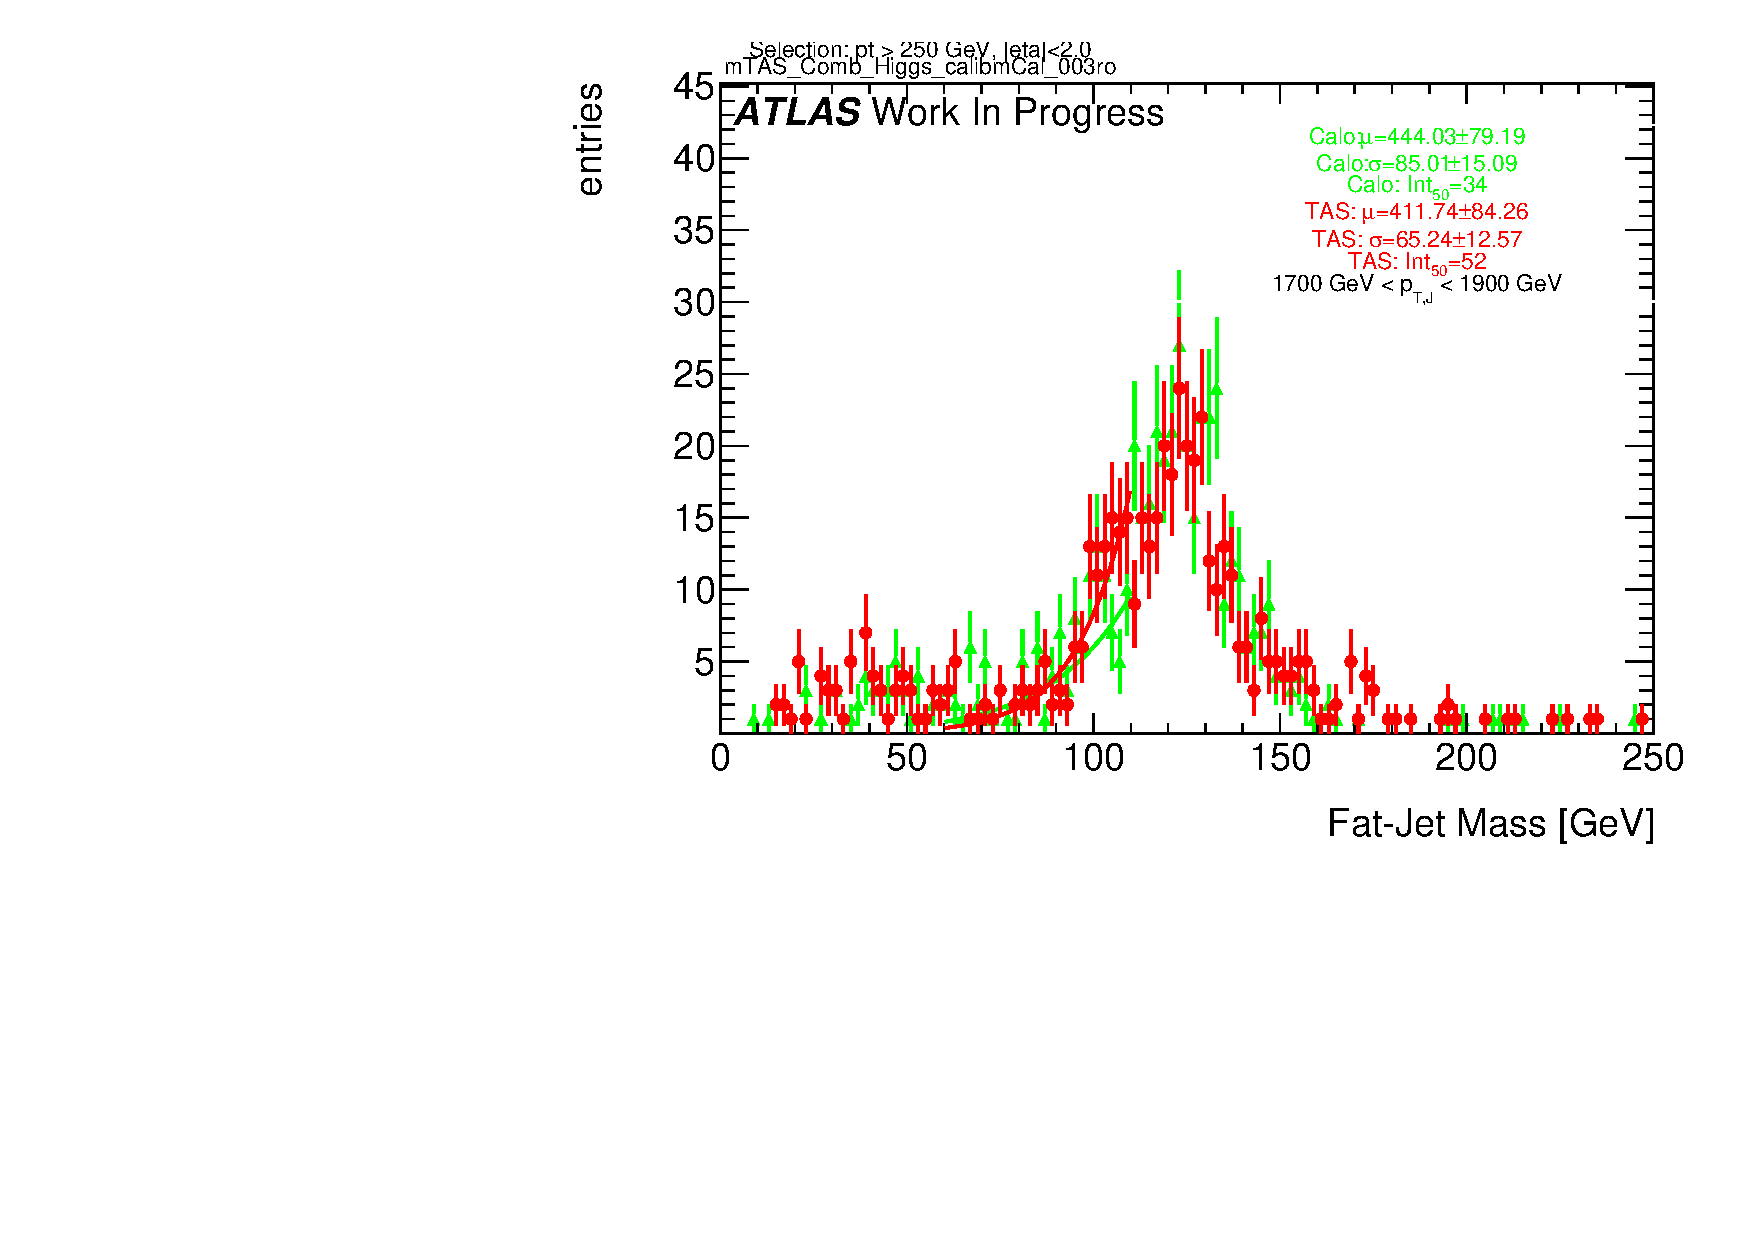
\includegraphics[width=0.4\textwidth]{/Users/fabnap/Documents/MasterArbeit/appendixB/mTAS_W_calibmCal_20:07:01-03-11-2016/12cfrt_h_FatJet_ptJ09m.pdf}
\caption{$\mtas$ and $\mcal$ for $p_{T}^{J}$ bin (indicated on plot) }
 
\end{figure}
 
\begin{figure}
 
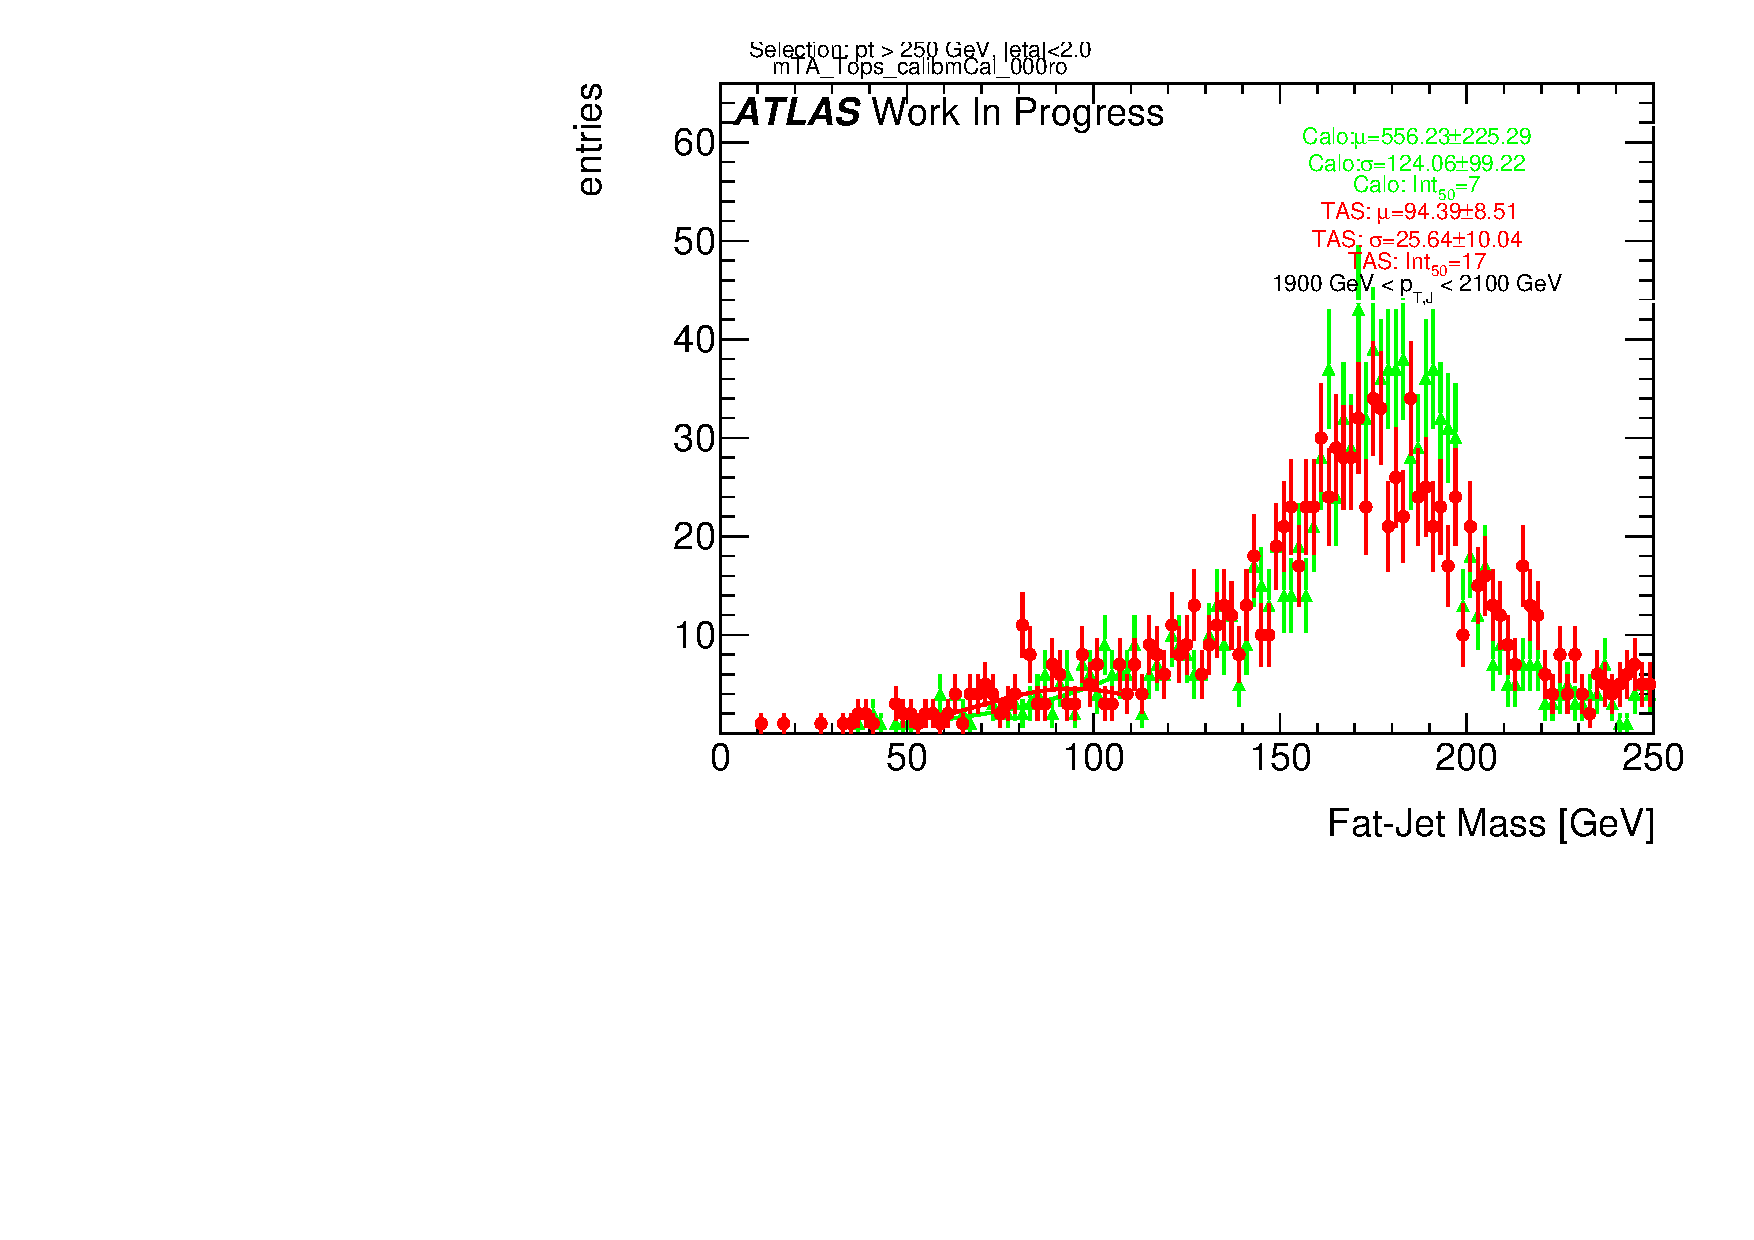
\includegraphics[width=0.4\textwidth]{/Users/fabnap/Documents/MasterArbeit/appendixB/mTAS_W_calibmCal_20:07:01-03-11-2016/12cfrt_h_FatJet_ptJ10m.pdf}
\caption{$\mtas$ and $\mcal$ for $p_{T}^{J}$ bin (indicated on plot) }
 
\end{figure}
 
\begin{figure}
 
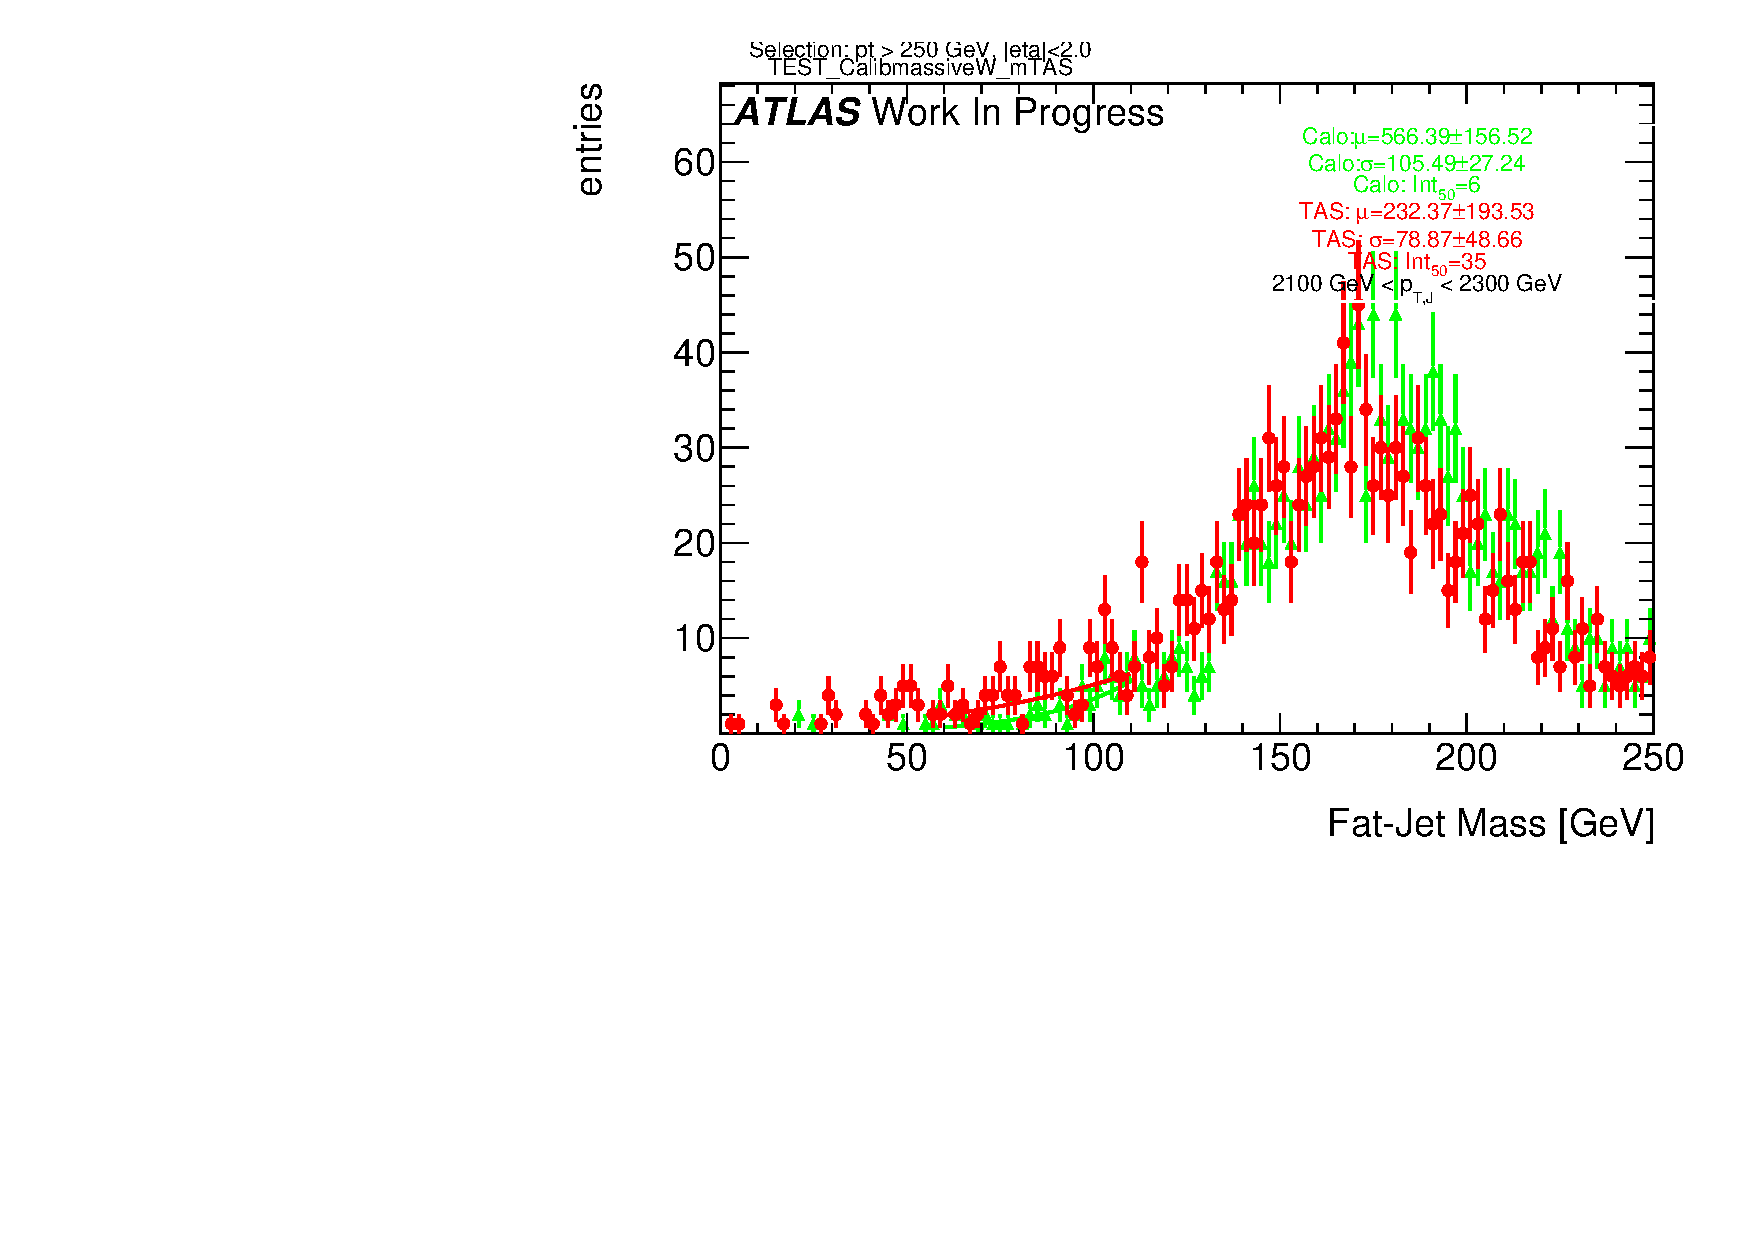
\includegraphics[width=0.4\textwidth]{/Users/fabnap/Documents/MasterArbeit/appendixB/mTAS_W_calibmCal_20:07:01-03-11-2016/12cfrt_h_FatJet_ptJ11m.pdf}
\caption{$\mtas$ and $\mcal$ for $p_{T}^{J}$ bin (indicated on plot) }
 
\end{figure}
 
\begin{figure}
 
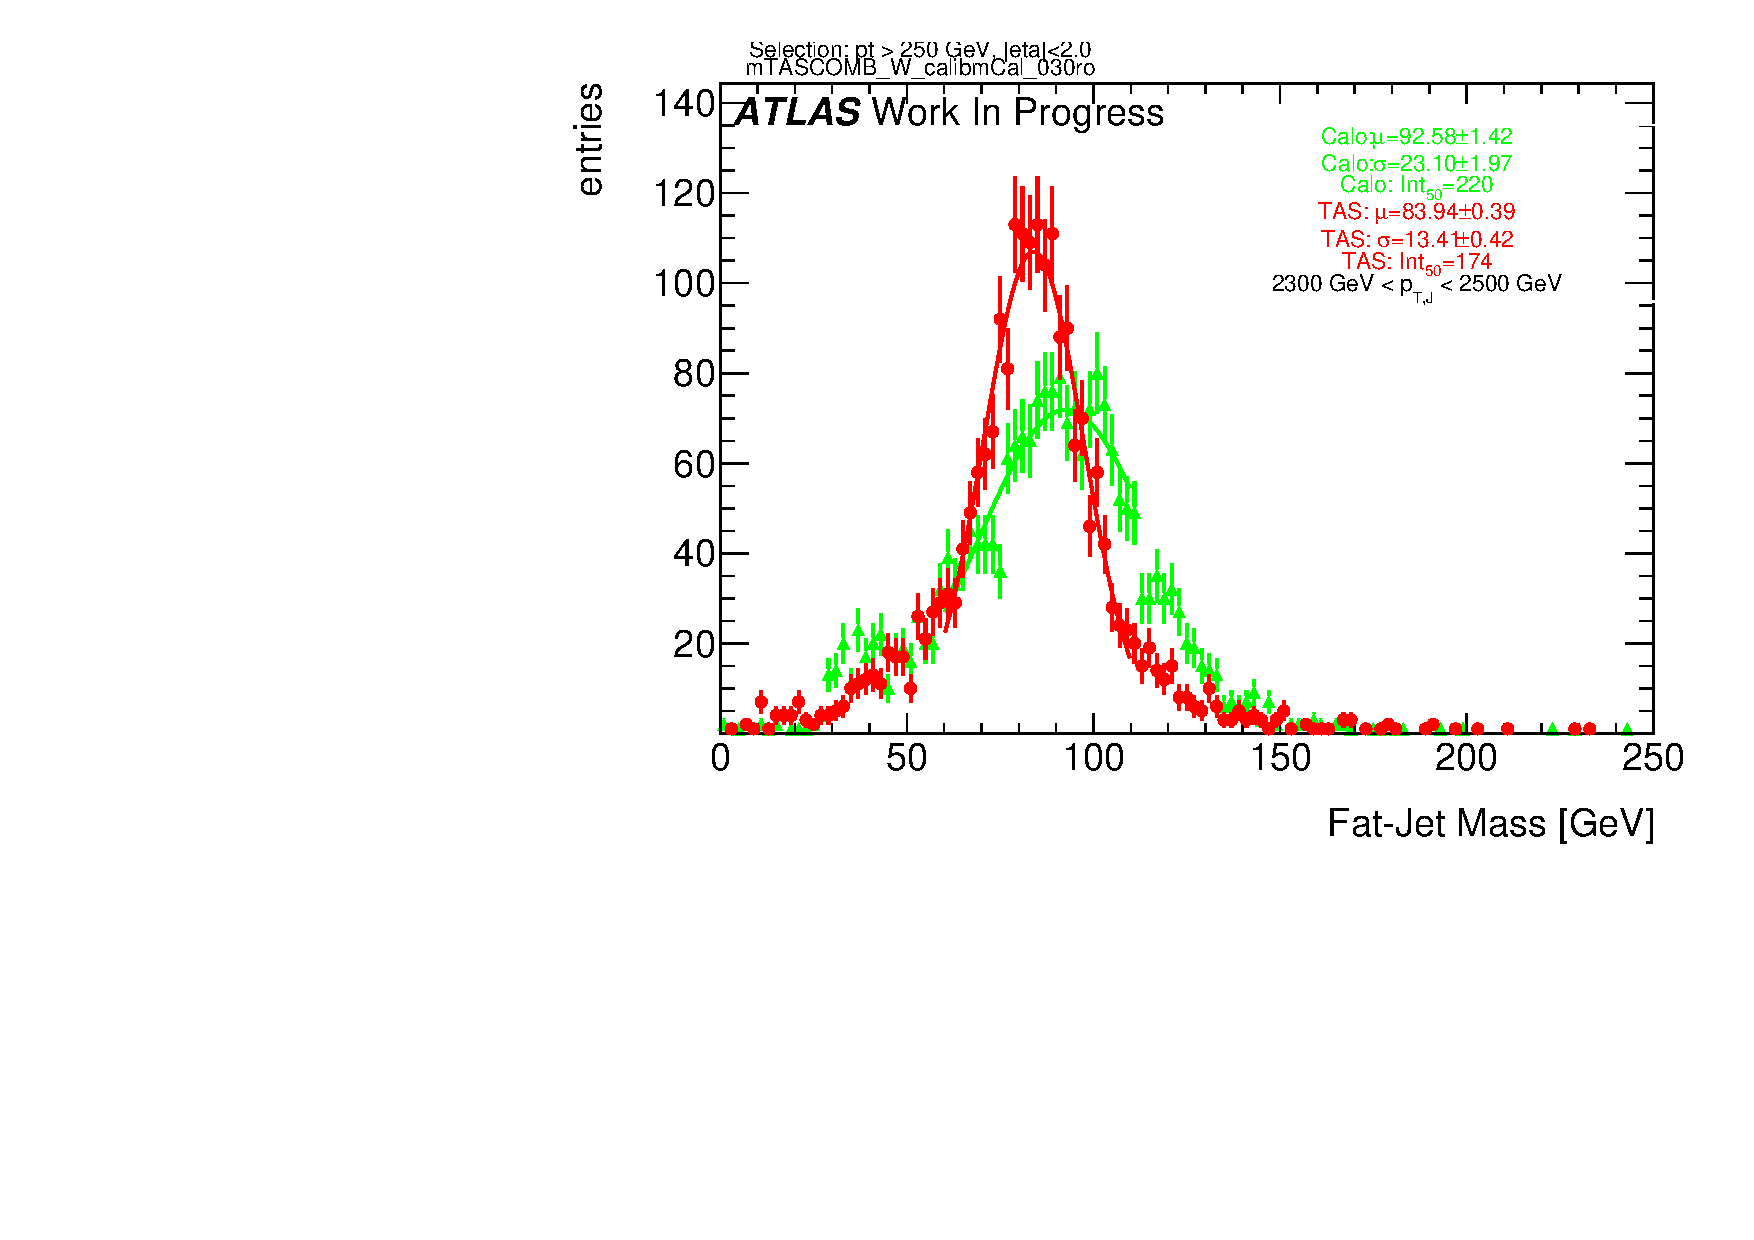
\includegraphics[width=0.4\textwidth]{/Users/fabnap/Documents/MasterArbeit/appendixB/mTAS_W_calibmCal_20:07:01-03-11-2016/12cfrt_h_FatJet_ptJ12m.pdf}
\caption{$\mtas$ and $\mcal$ for $p_{T}^{J}$ bin (indicated on plot) }
 
\end{figure}
\clearpage % 
\begin{figure}
 
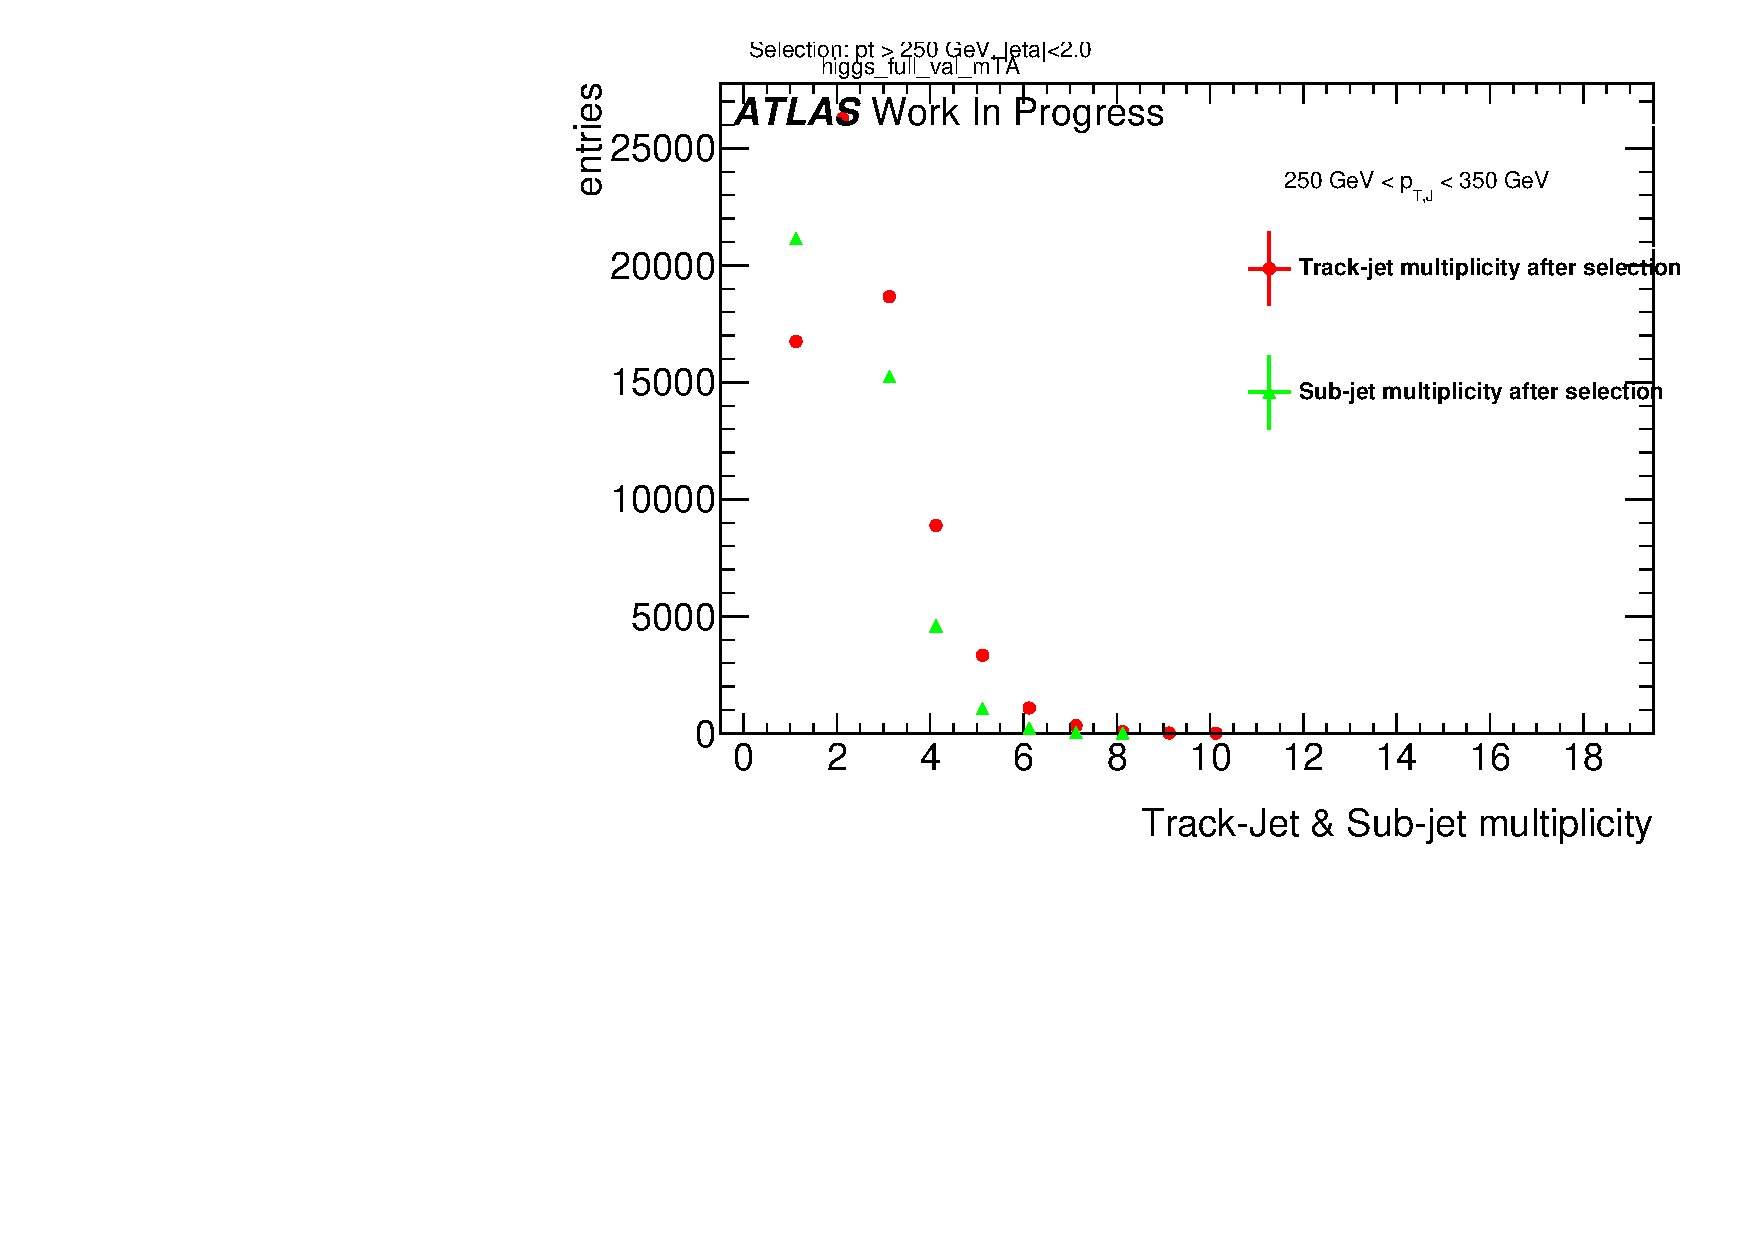
\includegraphics[width=0.4\textwidth]{/Users/fabnap/Documents/MasterArbeit/appendixB/mTAS_W_calibmCal_20:07:01-03-11-2016/13cfrt_h_SubJet_aftersel_ptJ01TAmult.pdf}
\caption{Track-jet R=0.2 and sub-jet multiplicity for $p_{T}^{J}$ bin (indicated on plot) }
 
\end{figure}
 
\begin{figure}
 
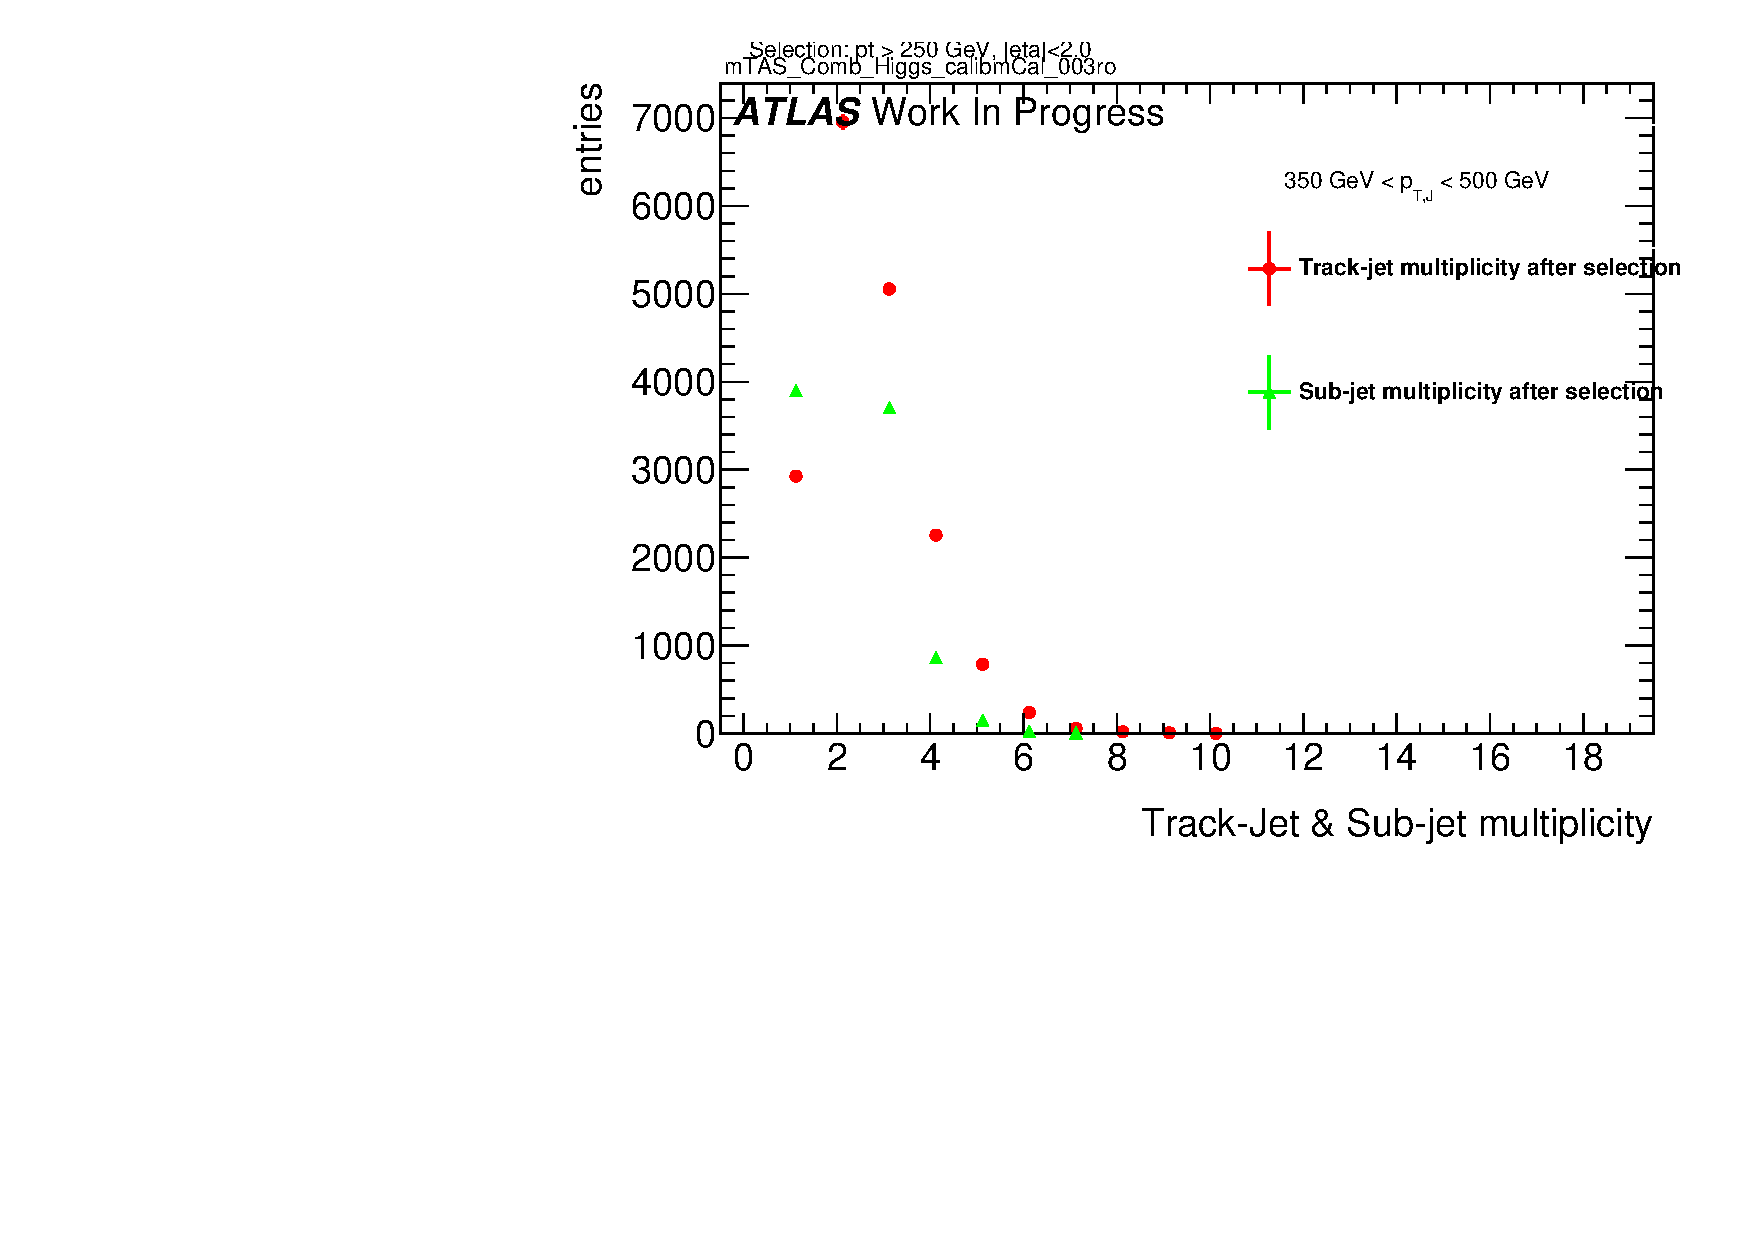
\includegraphics[width=0.4\textwidth]{/Users/fabnap/Documents/MasterArbeit/appendixB/mTAS_W_calibmCal_20:07:01-03-11-2016/13cfrt_h_SubJet_aftersel_ptJ02TAmult.pdf}
\caption{Track-jet R=0.2 and sub-jet multiplicity for $p_{T}^{J}$ bin (indicated on plot) }
 
\end{figure}
 
\begin{figure}
 
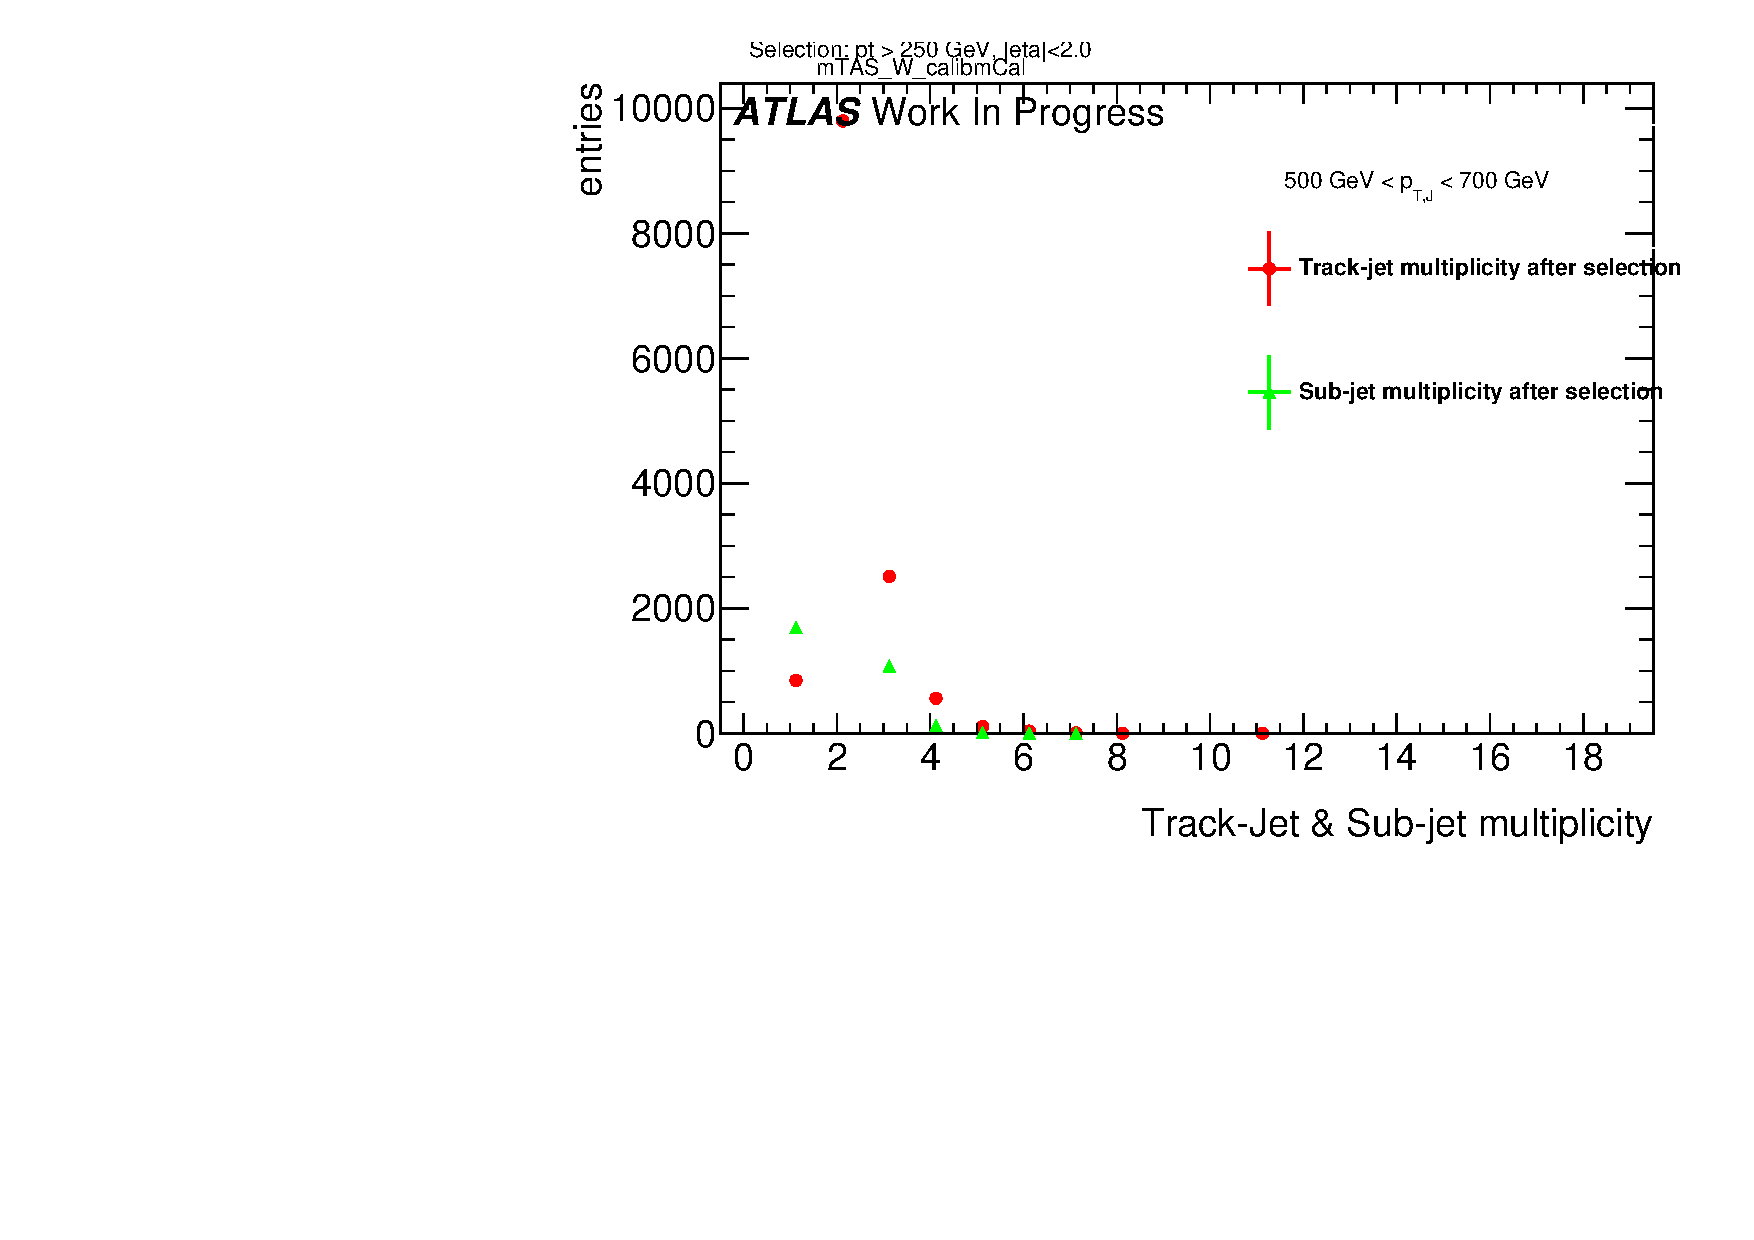
\includegraphics[width=0.4\textwidth]{/Users/fabnap/Documents/MasterArbeit/appendixB/mTAS_W_calibmCal_20:07:01-03-11-2016/13cfrt_h_SubJet_aftersel_ptJ03TAmult.pdf}
\caption{Track-jet R=0.2 and sub-jet multiplicity for $p_{T}^{J}$ bin (indicated on plot) }
 
\end{figure}
 
\begin{figure}
 
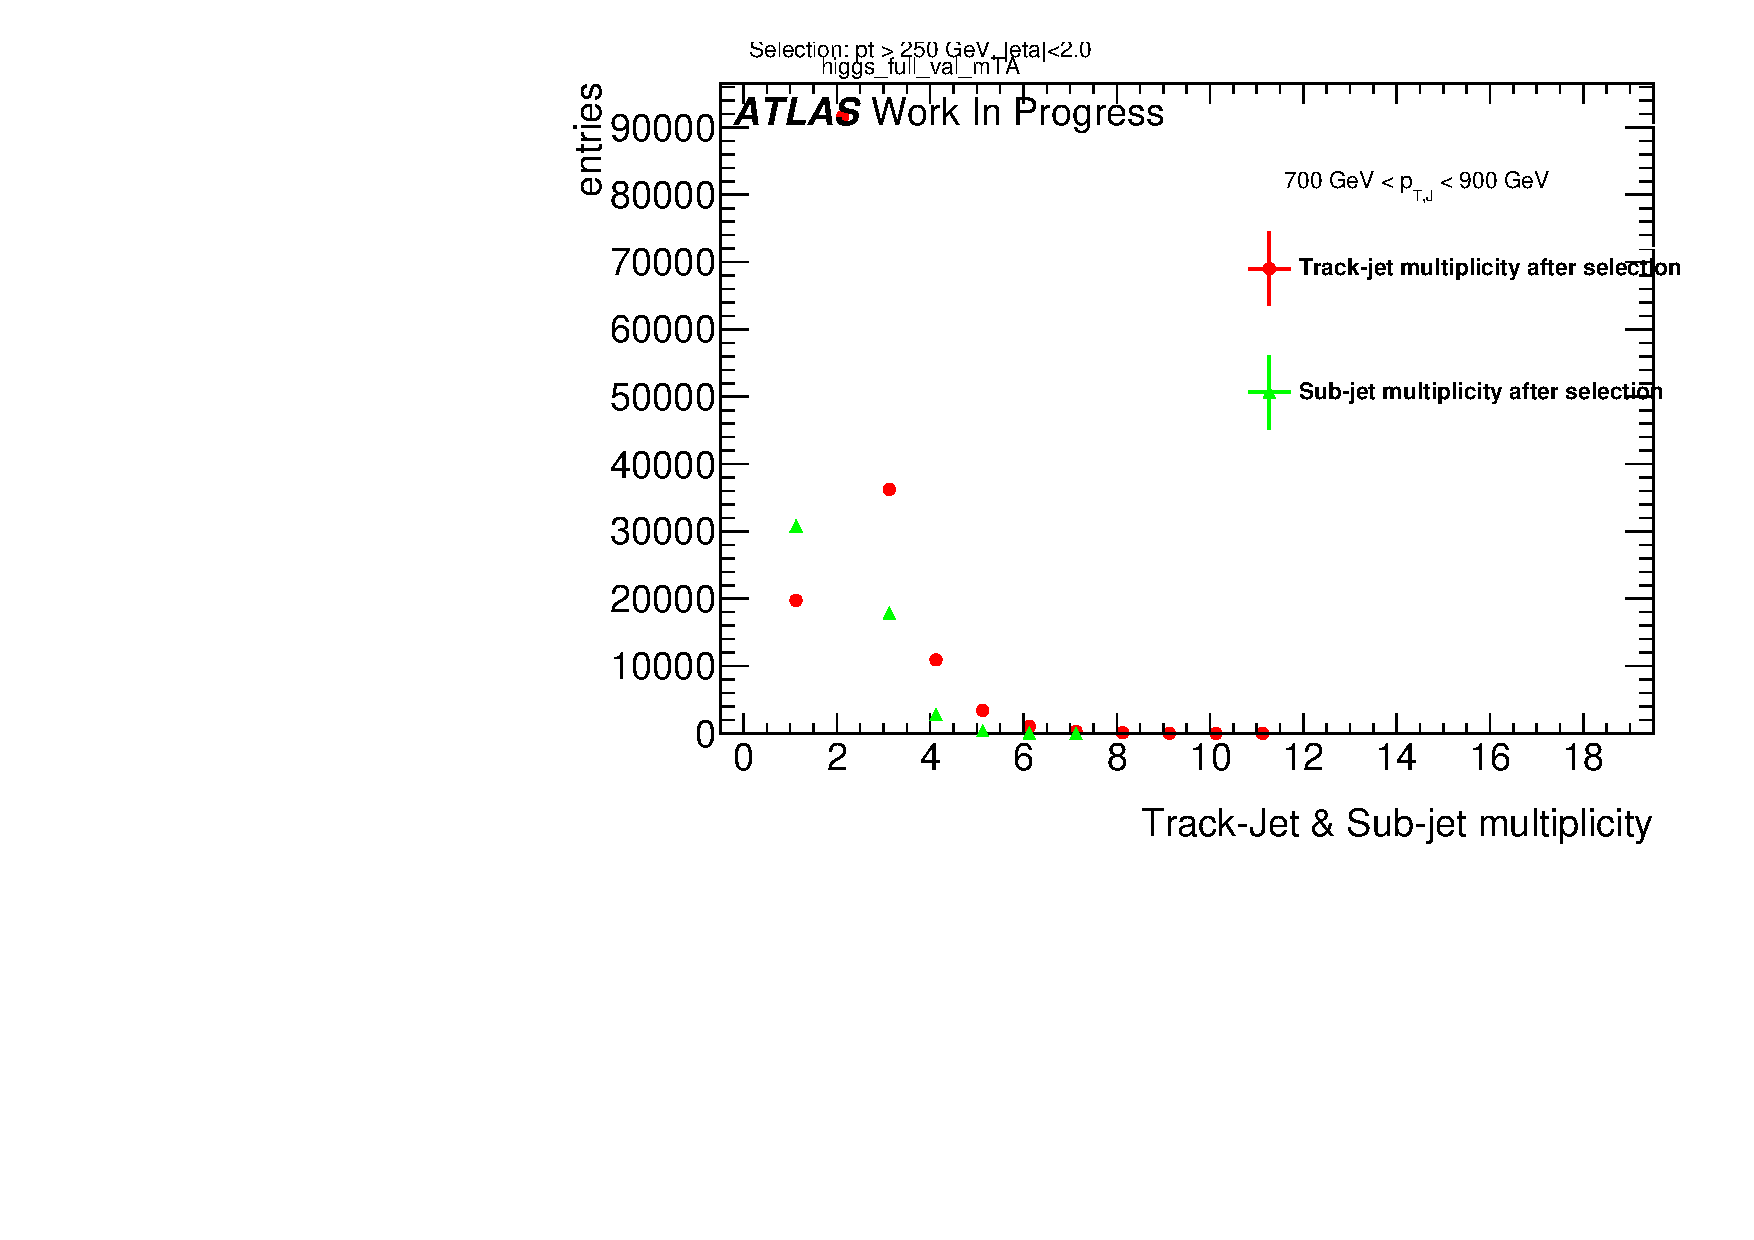
\includegraphics[width=0.4\textwidth]{/Users/fabnap/Documents/MasterArbeit/appendixB/mTAS_W_calibmCal_20:07:01-03-11-2016/13cfrt_h_SubJet_aftersel_ptJ04TAmult.pdf}
\caption{Track-jet R=0.2 and sub-jet multiplicity for $p_{T}^{J}$ bin (indicated on plot) }
 
\end{figure}
 
\begin{figure}
 
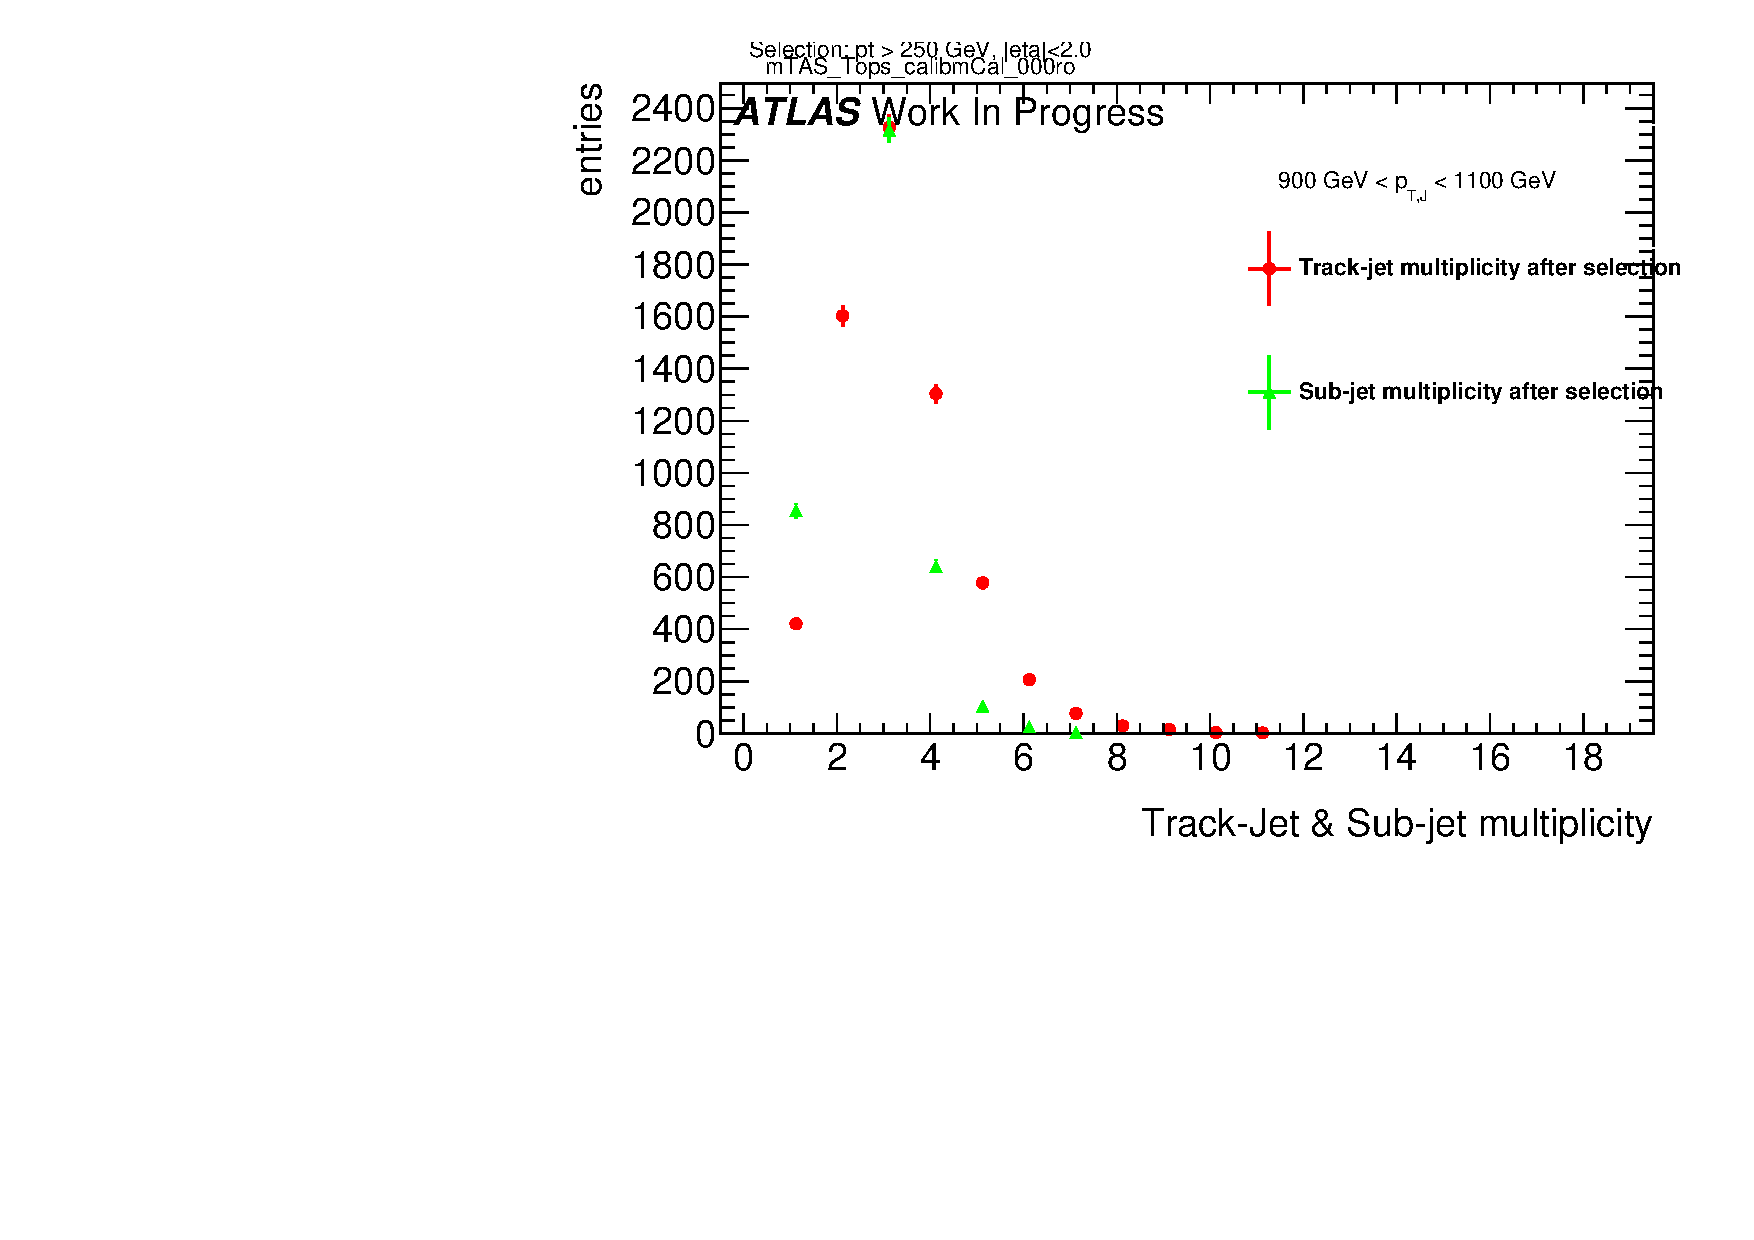
\includegraphics[width=0.4\textwidth]{/Users/fabnap/Documents/MasterArbeit/appendixB/mTAS_W_calibmCal_20:07:01-03-11-2016/13cfrt_h_SubJet_aftersel_ptJ05TAmult.pdf}
\caption{Track-jet R=0.2 and sub-jet multiplicity for $p_{T}^{J}$ bin (indicated on plot) }
 
\end{figure}
 
\begin{figure}
 
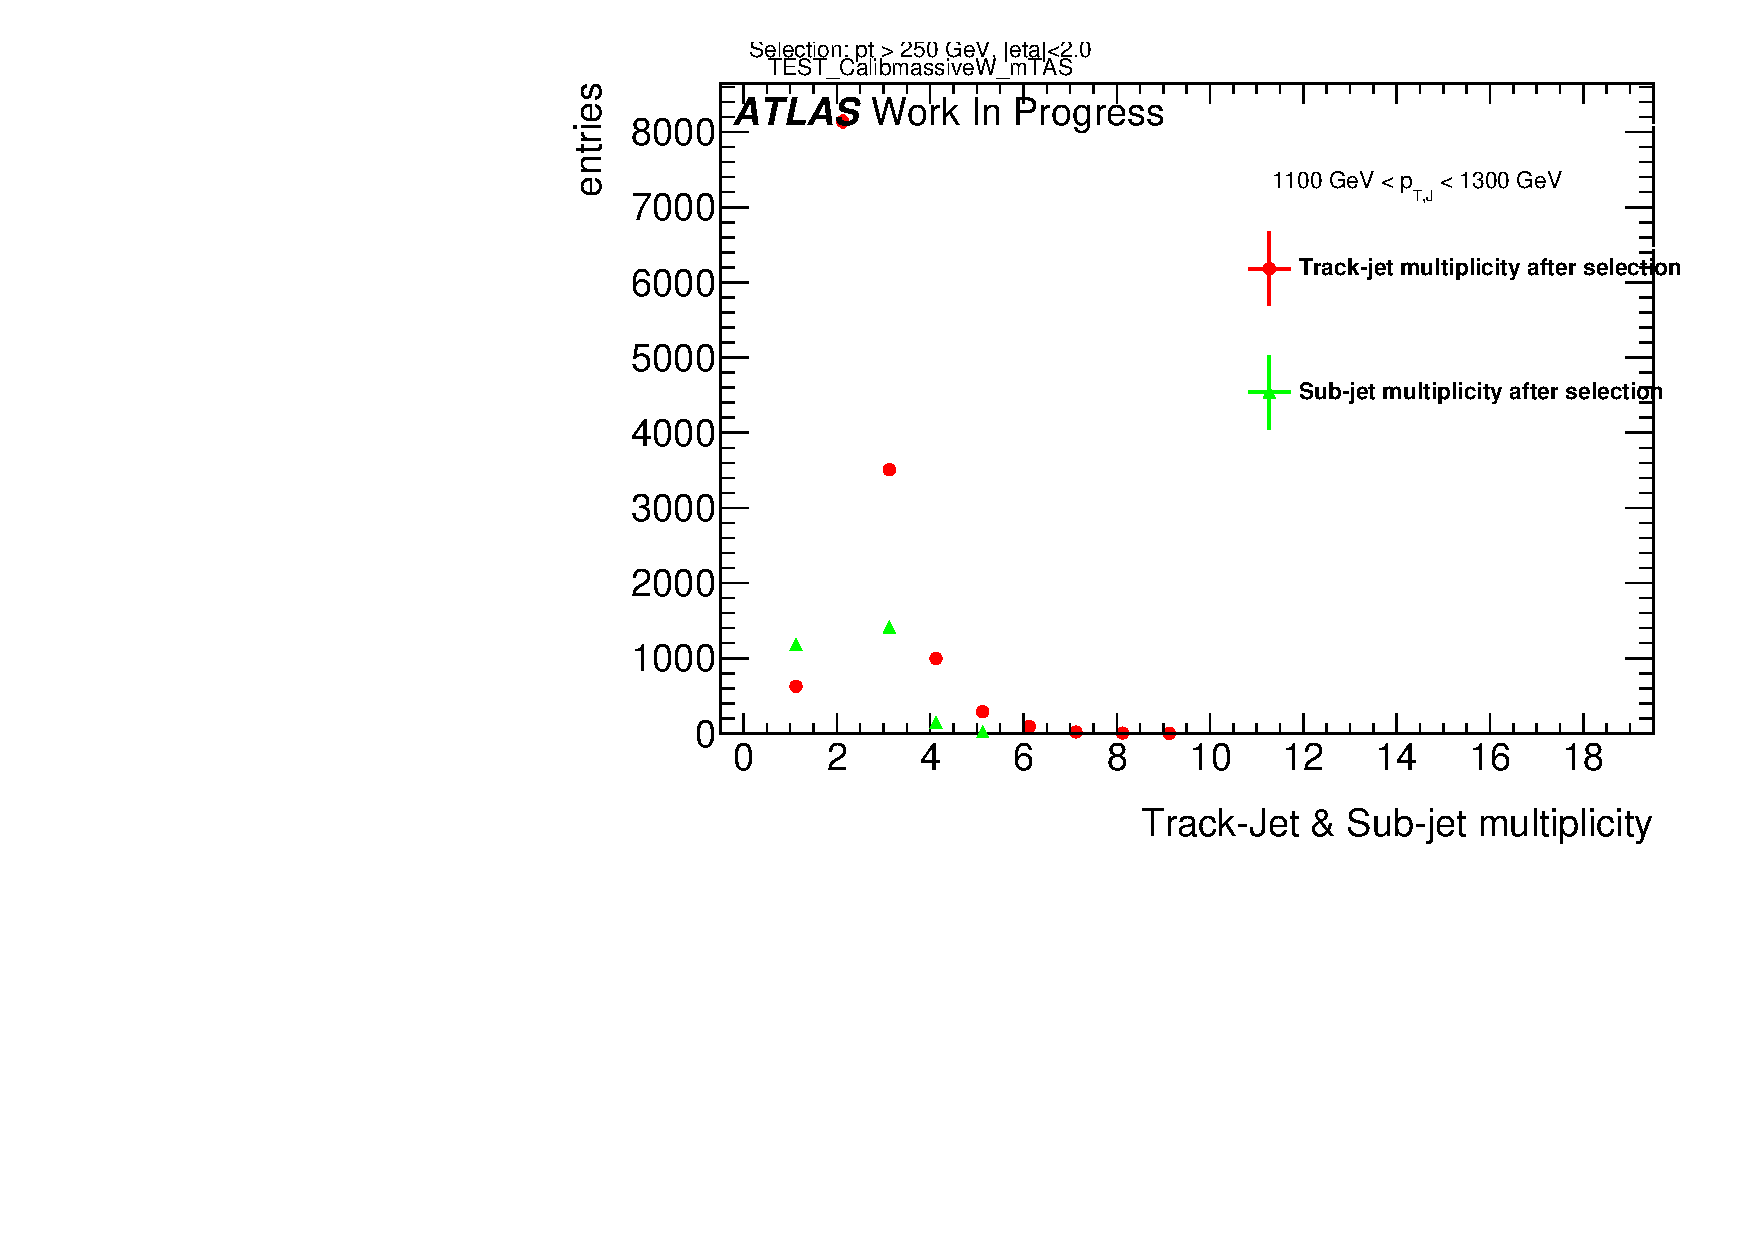
\includegraphics[width=0.4\textwidth]{/Users/fabnap/Documents/MasterArbeit/appendixB/mTAS_W_calibmCal_20:07:01-03-11-2016/13cfrt_h_SubJet_aftersel_ptJ06TAmult.pdf}
\caption{Track-jet R=0.2 and sub-jet multiplicity for $p_{T}^{J}$ bin (indicated on plot) }
 
\end{figure}
 %
\begin{figure}
 
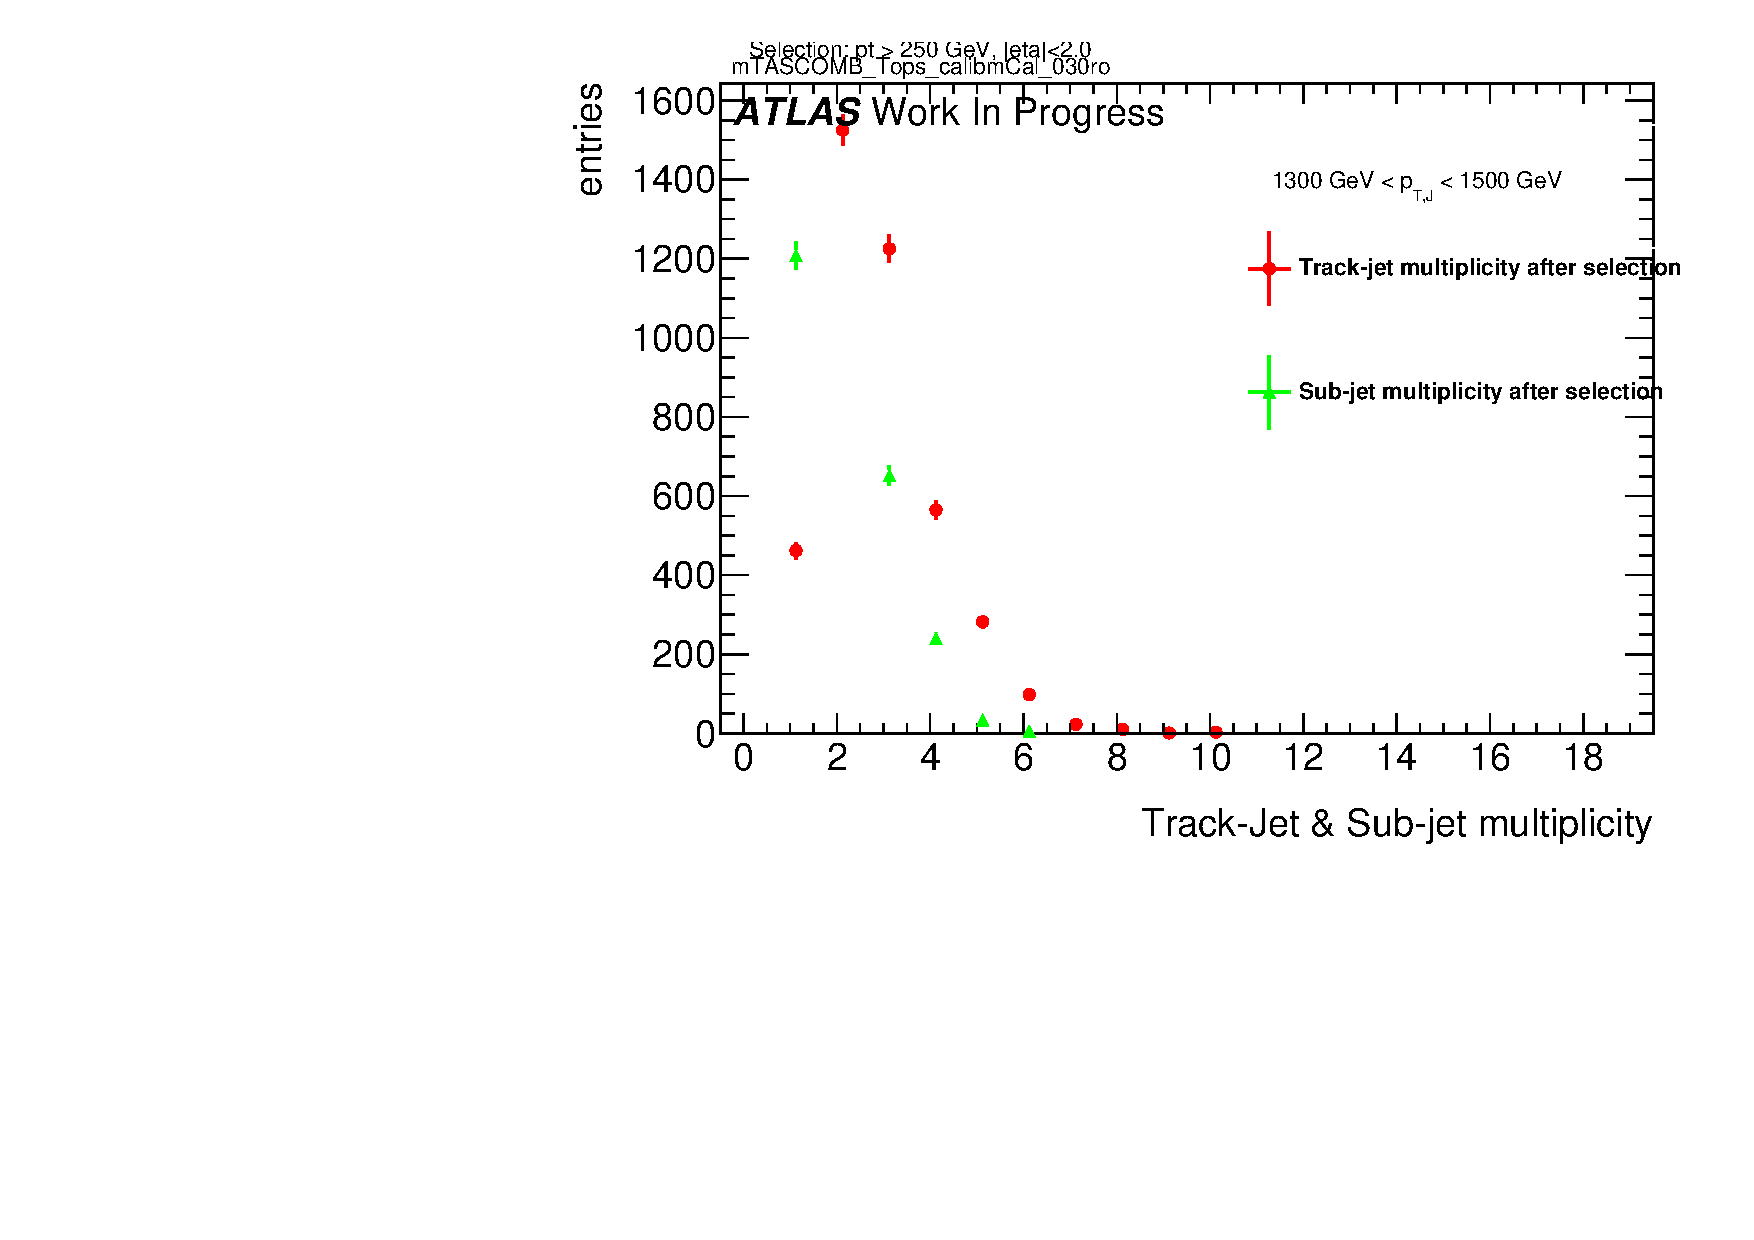
\includegraphics[width=0.4\textwidth]{/Users/fabnap/Documents/MasterArbeit/appendixB/mTAS_W_calibmCal_20:07:01-03-11-2016/13cfrt_h_SubJet_aftersel_ptJ07TAmult.pdf}
\caption{Track-jet R=0.2 and sub-jet multiplicity for $p_{T}^{J}$ bin (indicated on plot) }
 
\end{figure}
 
\begin{figure}
 
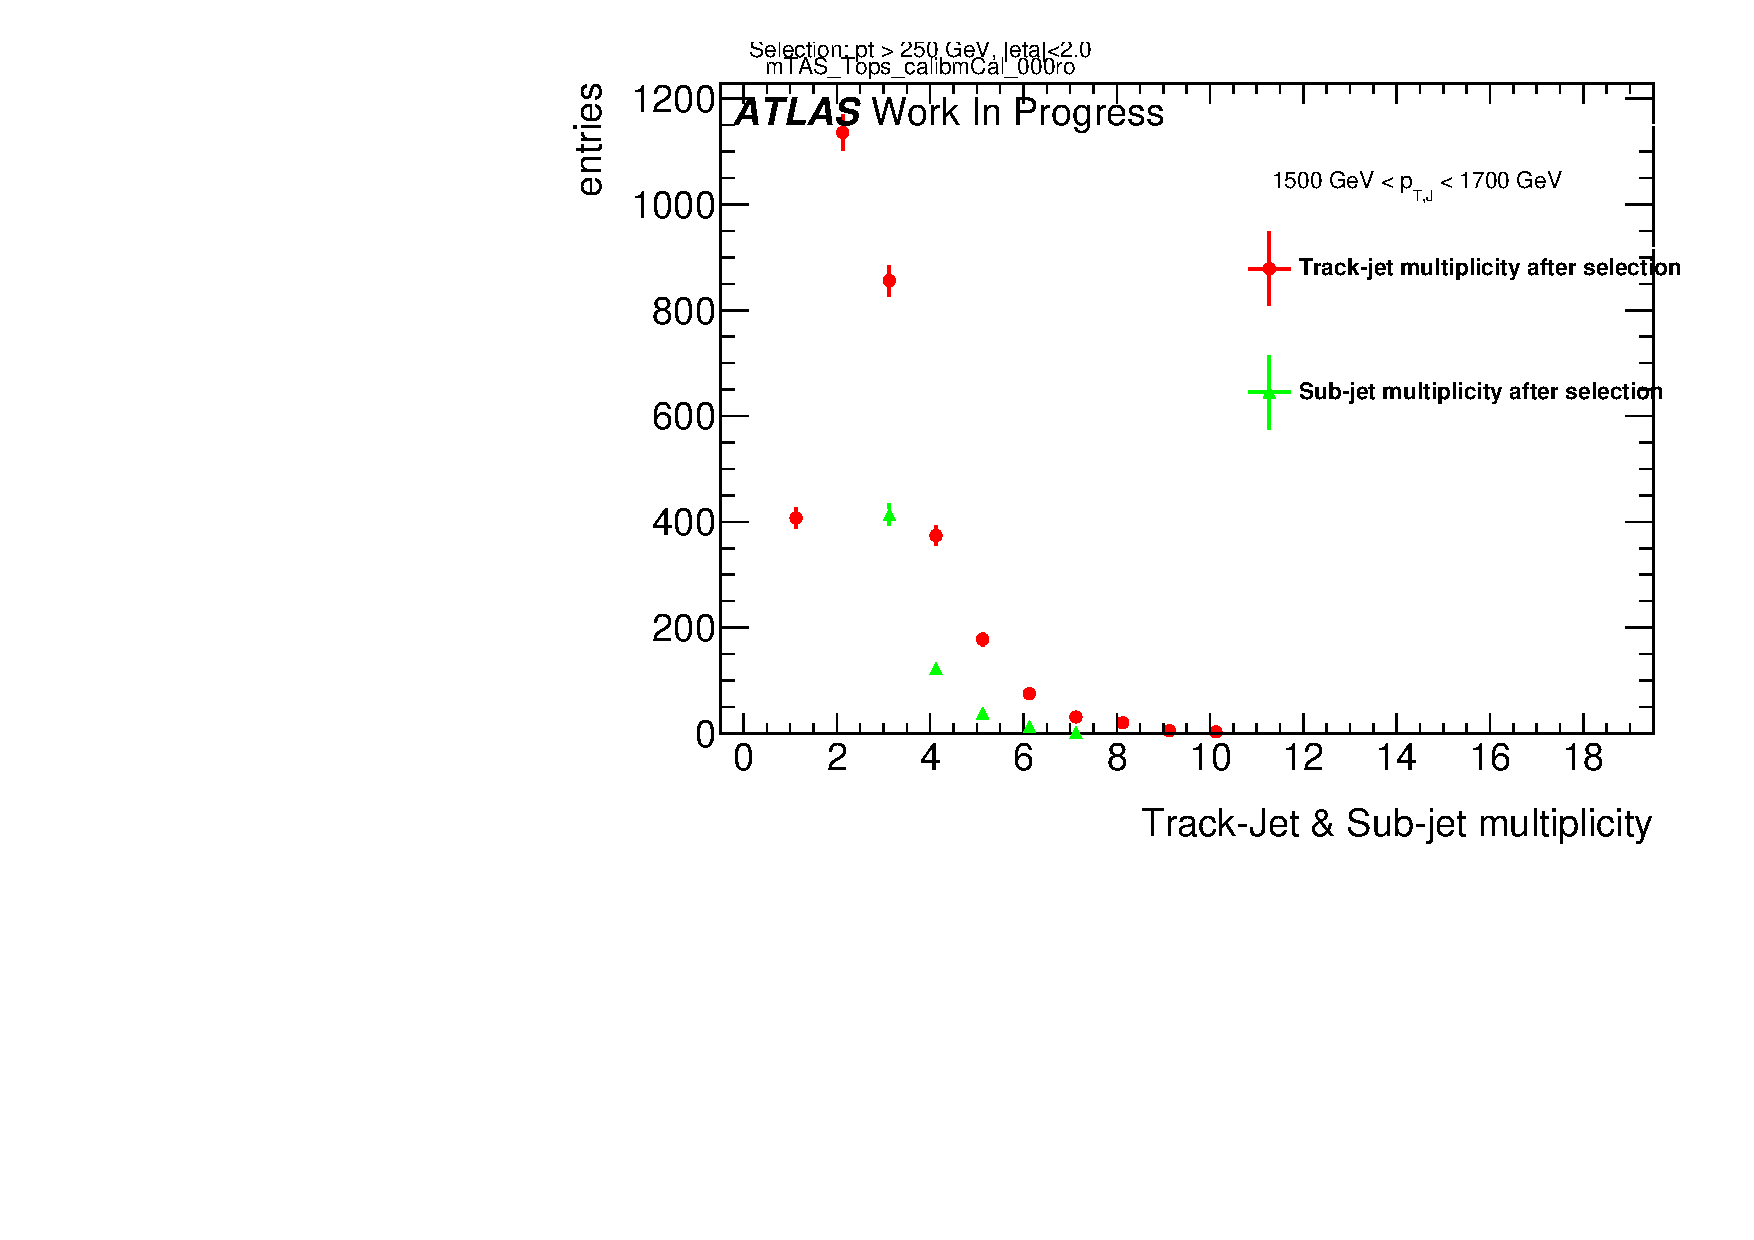
\includegraphics[width=0.4\textwidth]{/Users/fabnap/Documents/MasterArbeit/appendixB/mTAS_W_calibmCal_20:07:01-03-11-2016/13cfrt_h_SubJet_aftersel_ptJ08TAmult.pdf}
\caption{Track-jet R=0.2 and sub-jet multiplicity for $p_{T}^{J}$ bin (indicated on plot) }
 
\end{figure}

\begin{figure}

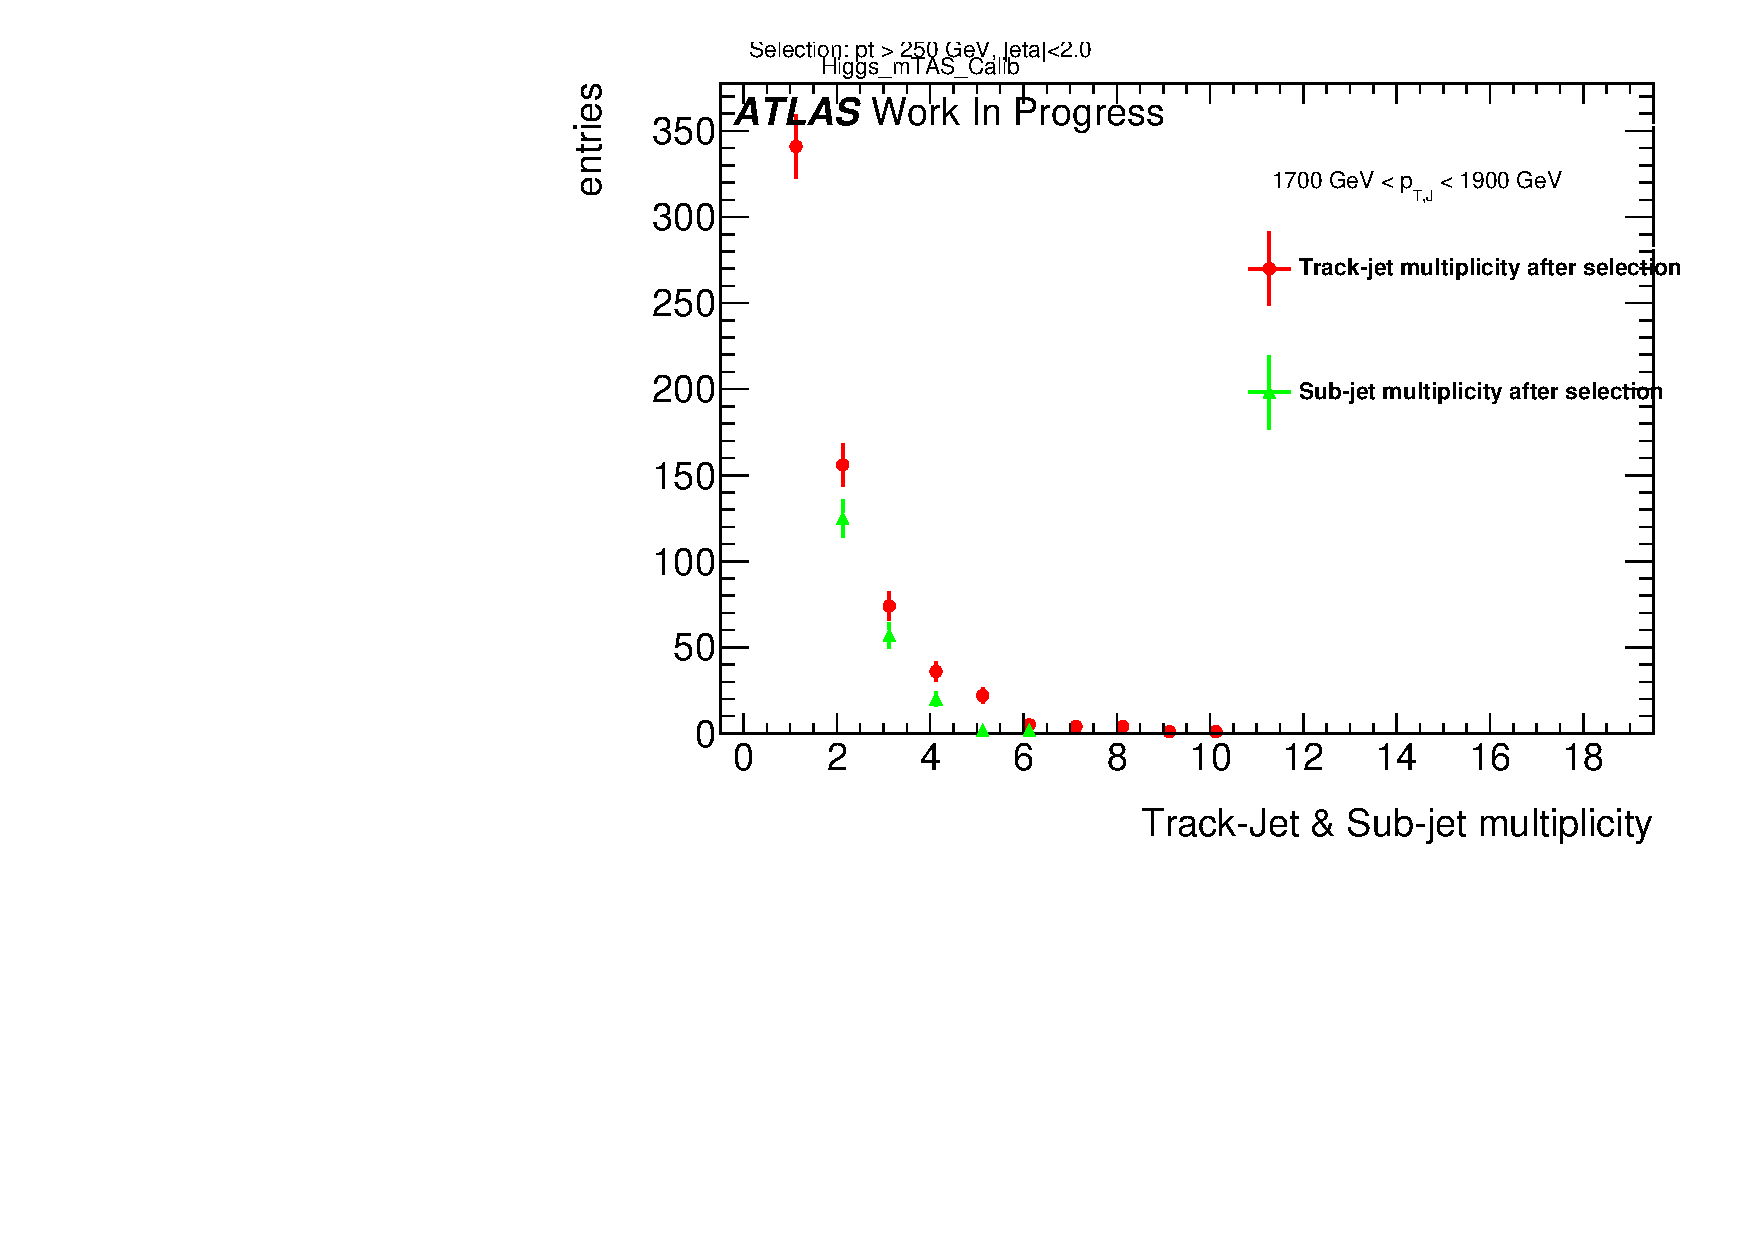
\includegraphics[width=0.4\textwidth]{/Users/fabnap/Documents/MasterArbeit/appendixB/mTAS_W_calibmCal_20:07:01-03-11-2016/13cfrt_h_SubJet_aftersel_ptJ09TAmult.pdf}
\caption{Track-jet R=0.2 and sub-jet multiplicity for $p_{T}^{J}$ bin (indicated on plot) }
 
\end{figure}
 
\begin{figure}

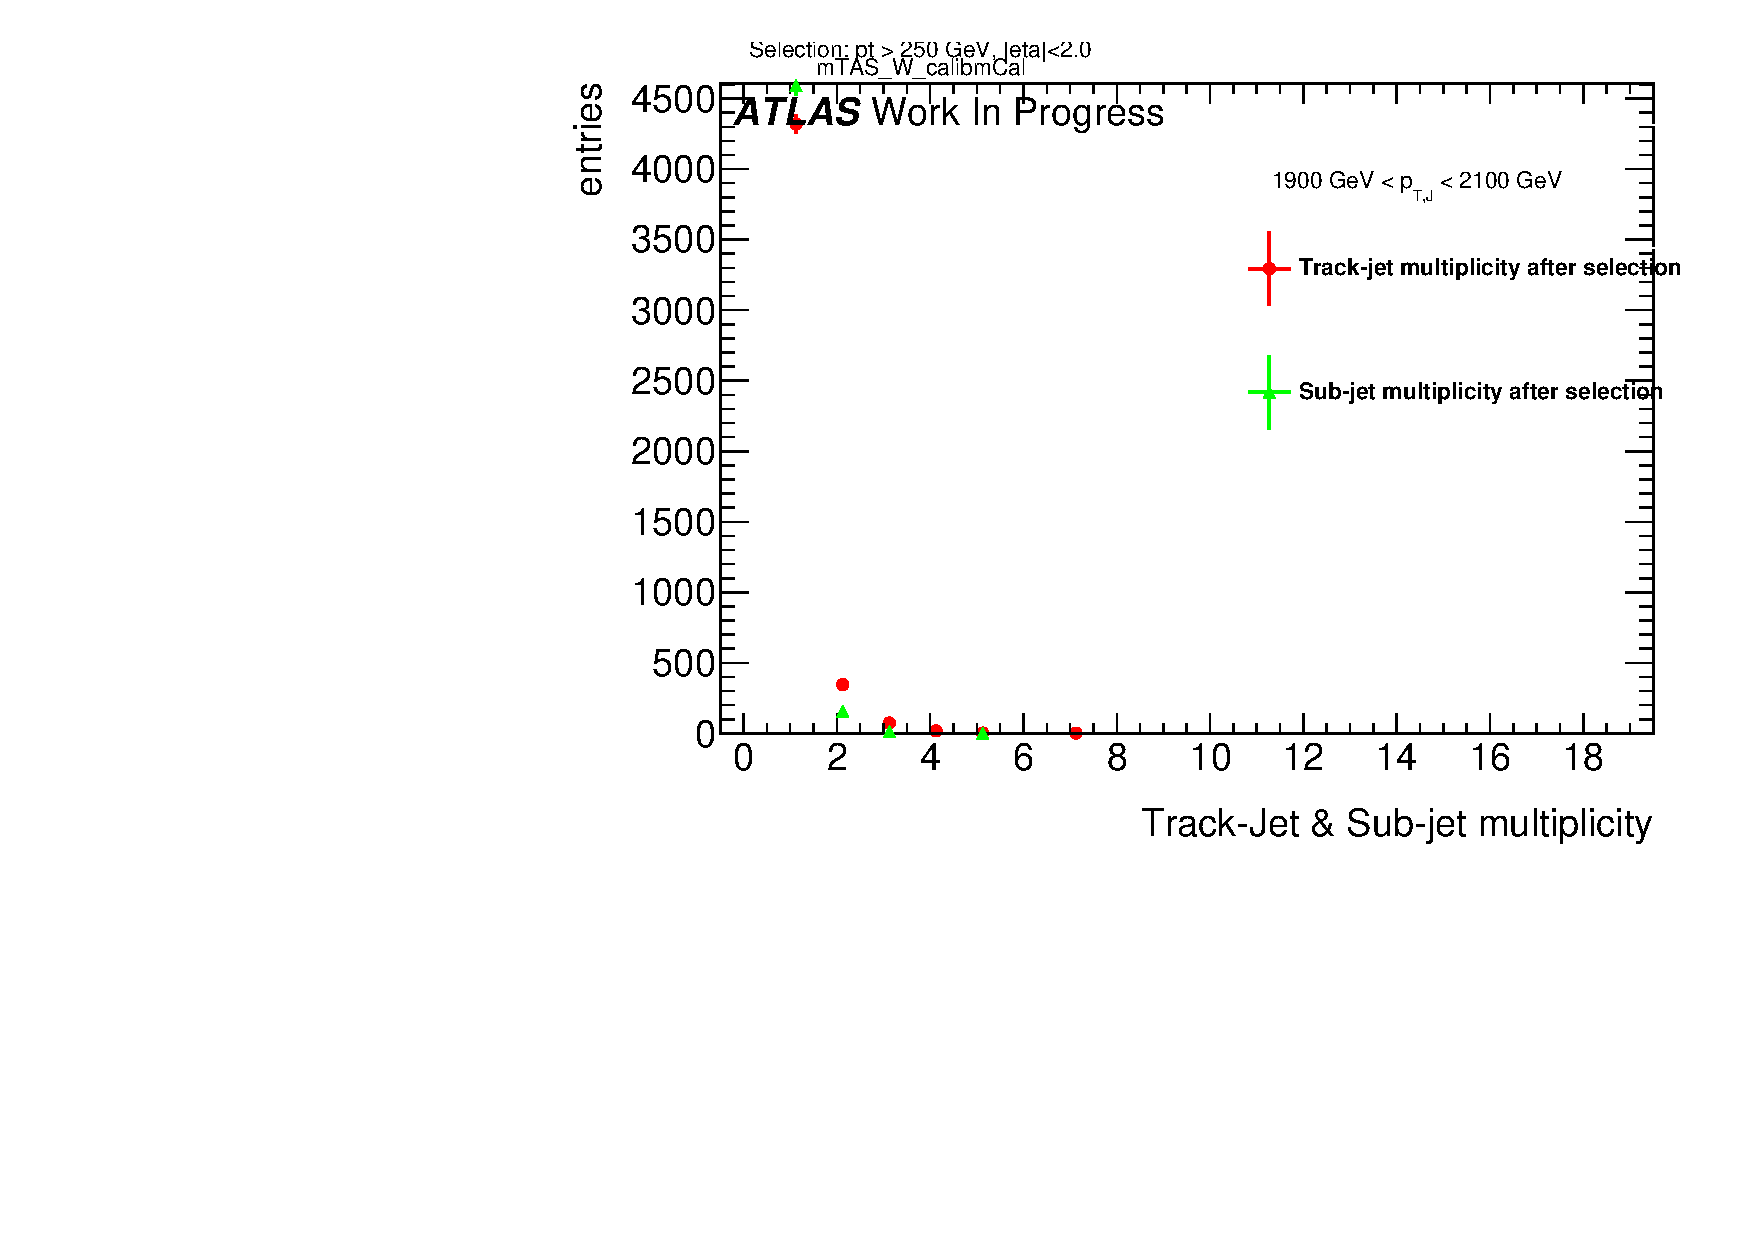
\includegraphics[width=0.4\textwidth]{/Users/fabnap/Documents/MasterArbeit/appendixB/mTAS_W_calibmCal_20:07:01-03-11-2016/13cfrt_h_SubJet_aftersel_ptJ10TAmult.pdf}
\caption{Track-jet R=0.2 and sub-jet multiplicity for $p_{T}^{J}$ bin (indicated on plot) }

\end{figure}

\begin{figure}

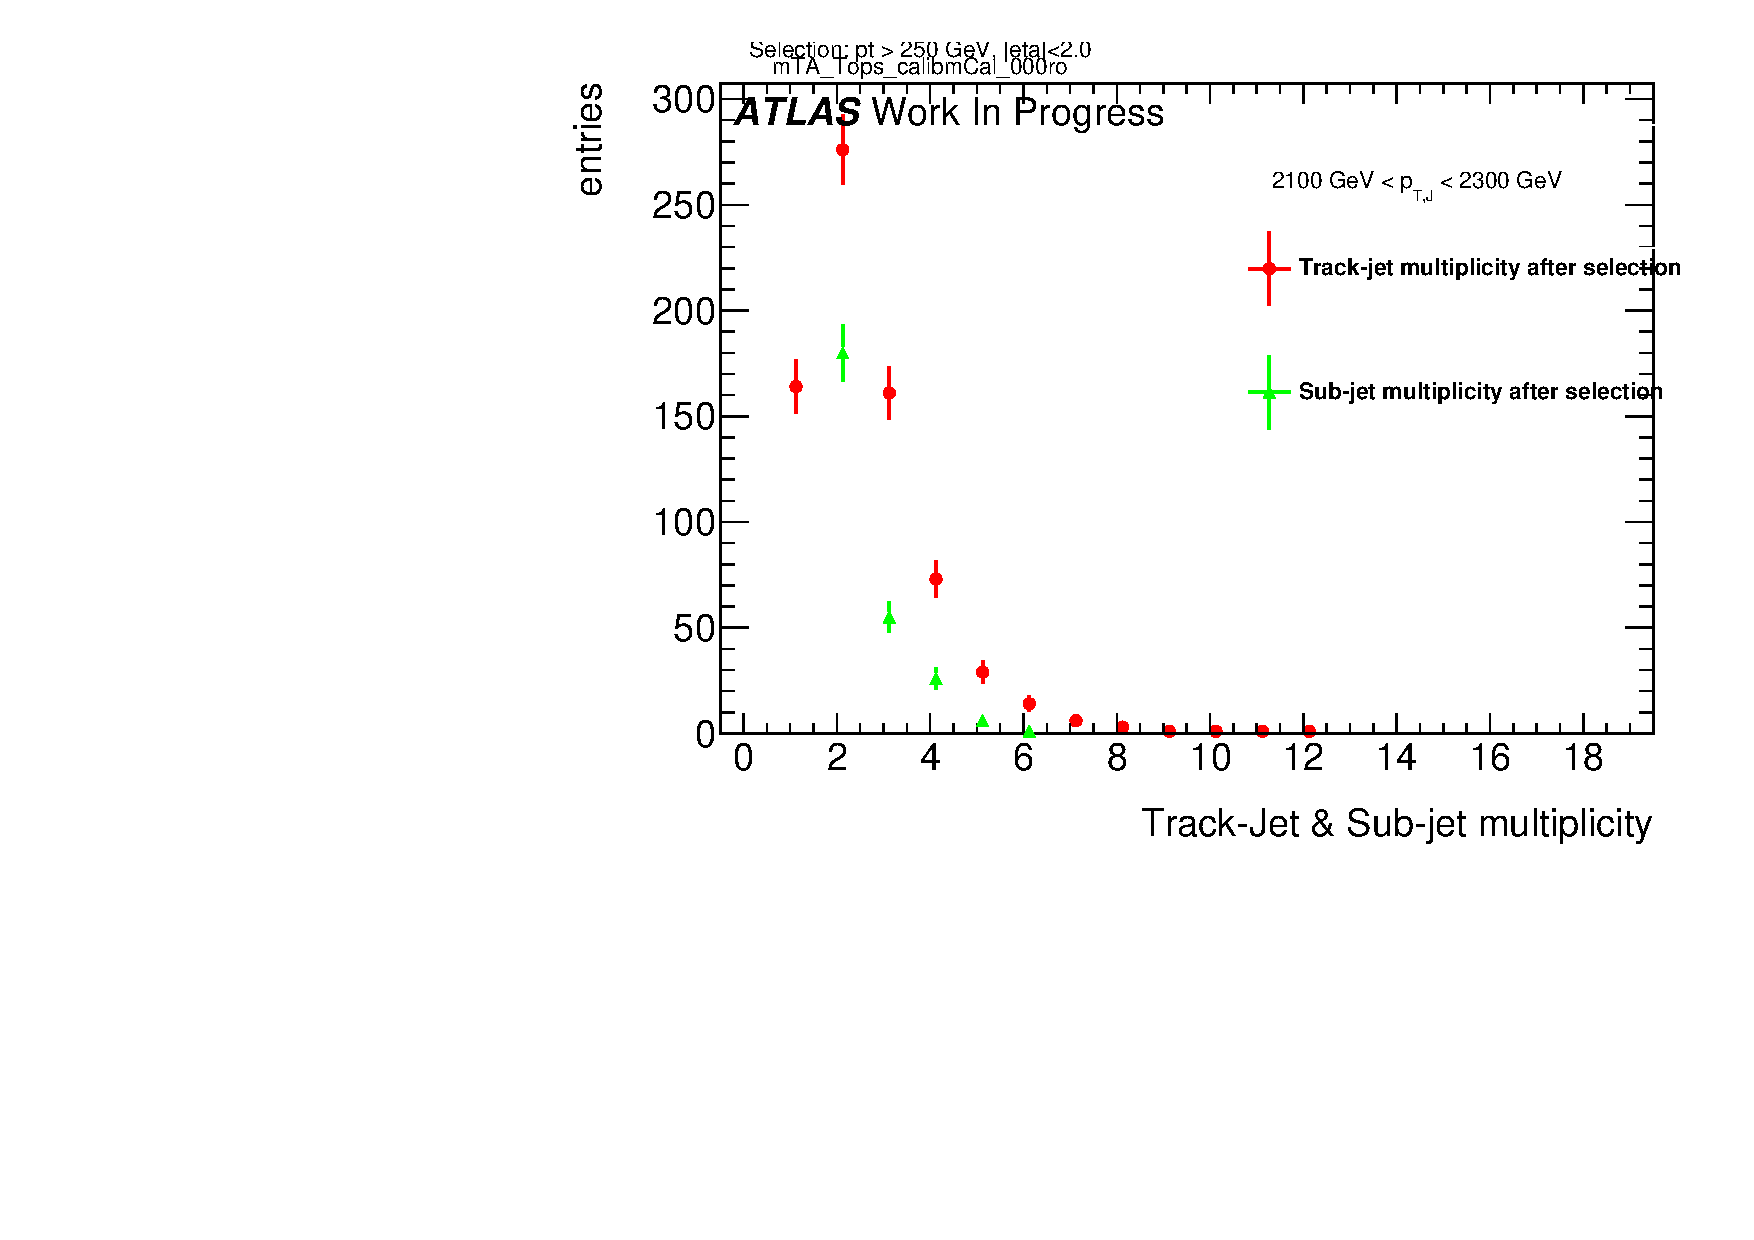
\includegraphics[width=0.4\textwidth]{/Users/fabnap/Documents/MasterArbeit/appendixB/mTAS_W_calibmCal_20:07:01-03-11-2016/13cfrt_h_SubJet_aftersel_ptJ11TAmult.pdf}
\caption{Track-jet R=0.2 and sub-jet multiplicity for $p_{T}^{J}$ bin (indicated on plot) }

\end{figure}

\begin{figure}

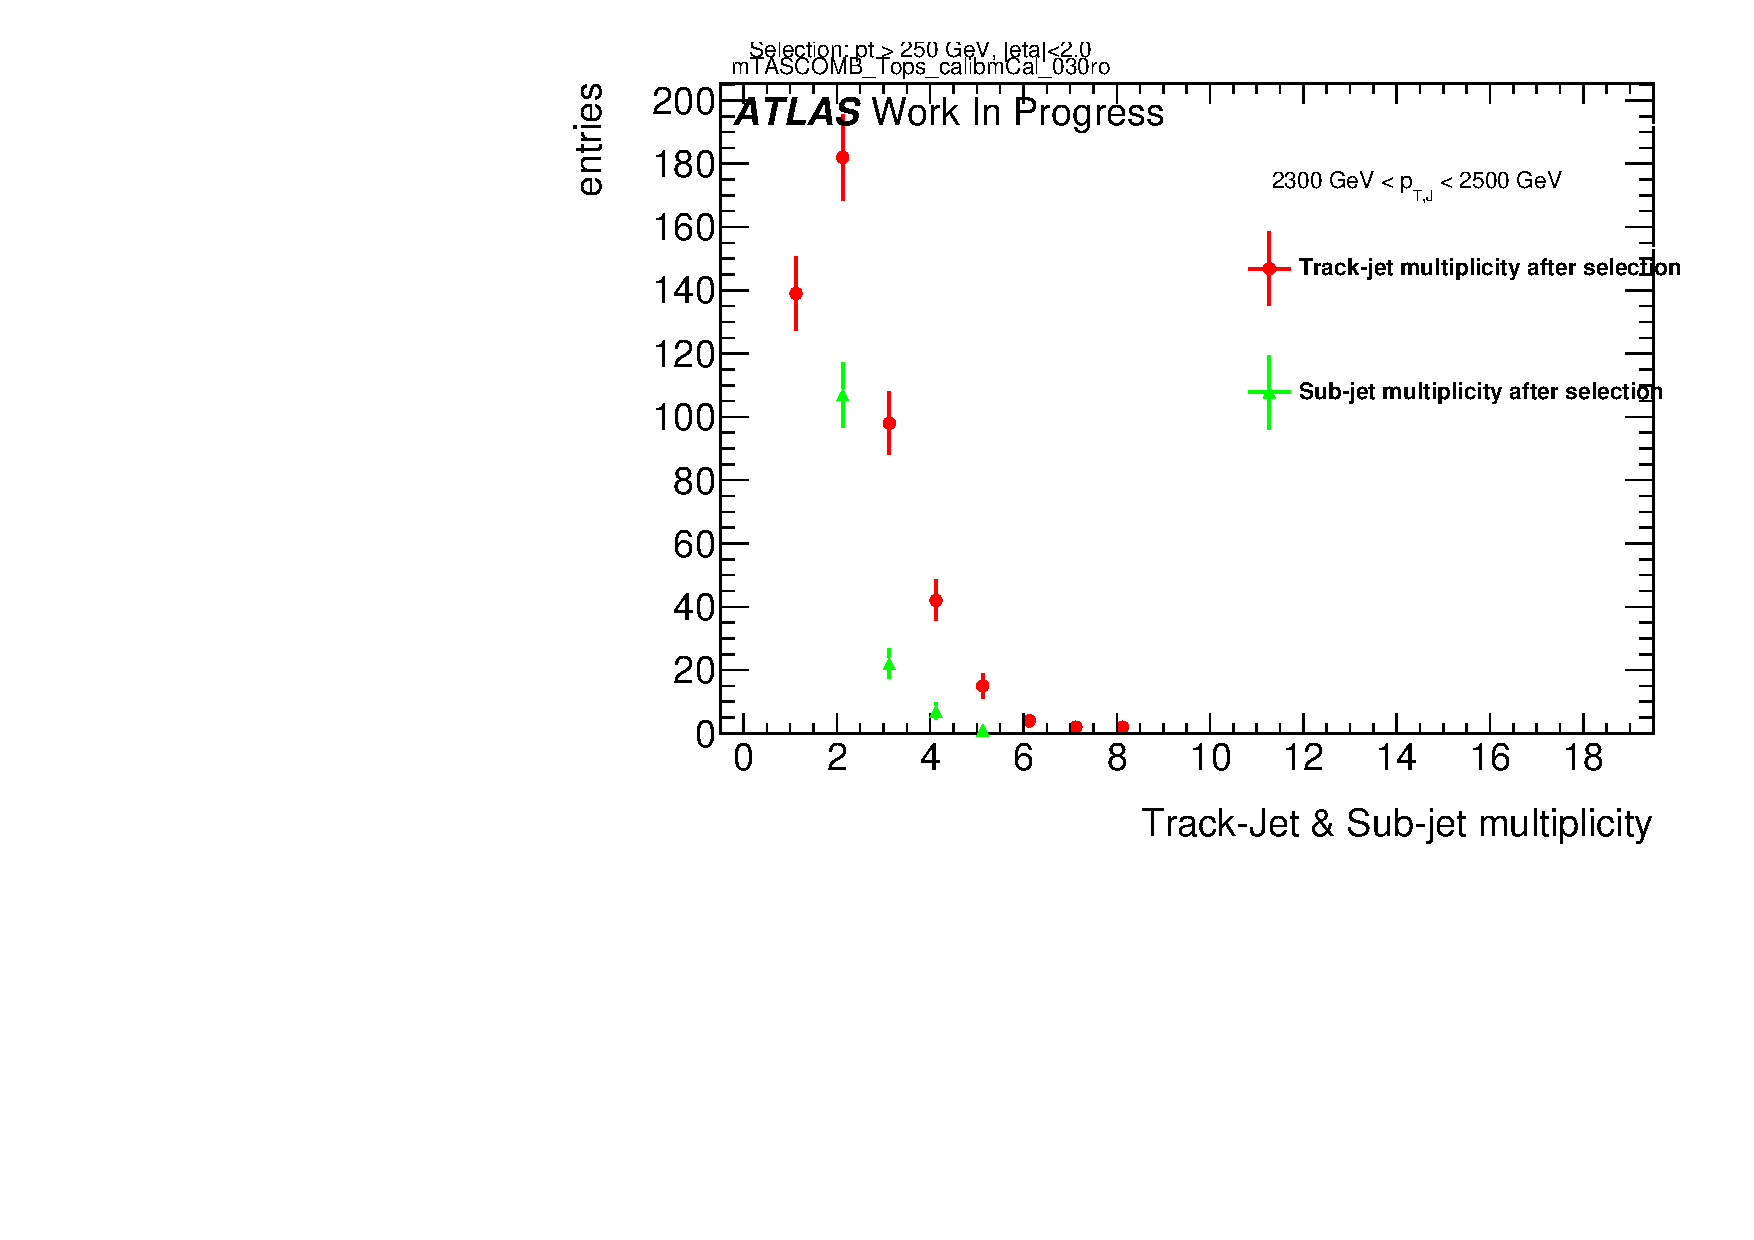
\includegraphics[width=0.4\textwidth]{/Users/fabnap/Documents/MasterArbeit/appendixB/mTAS_W_calibmCal_20:07:01-03-11-2016/13cfrt_h_SubJet_aftersel_ptJ12TAmult.pdf}
\caption{Track-jet R=0.2 and sub-jet multiplicity for $p_{T}^{J}$ bin (indicated on plot) }

\end{figure}

\clearpage

\begin{figure}

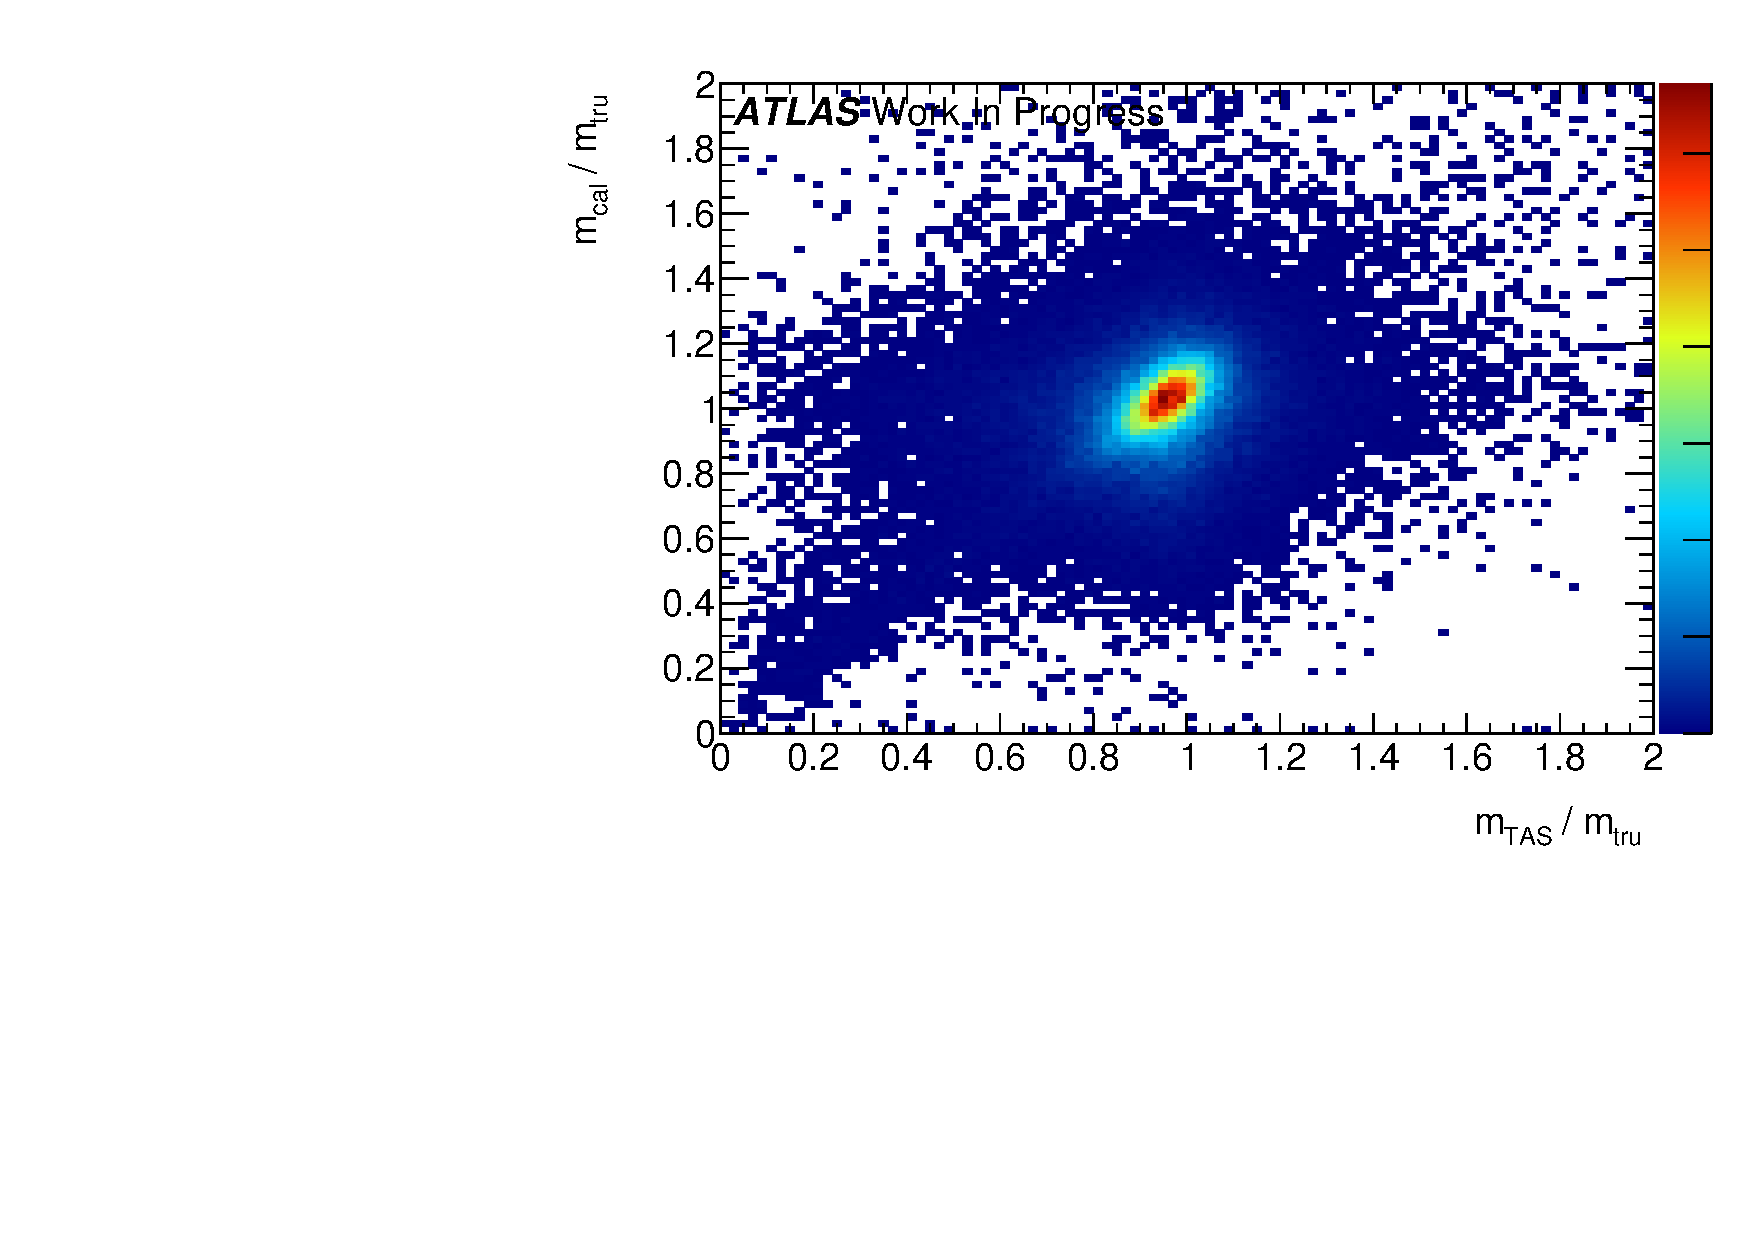
\includegraphics[width=0.4\textwidth]{/Users/fabnap/Documents/MasterArbeit/appendixB/mTAS_W_calibmCal_20:07:01-03-11-2016/1cfrt_h_fabsca_tascal_2.pdf}
\caption{Scatter plot $\mtas$ versus $\mcal$ responses}

\end{figure}
 
\begin{figure}
 
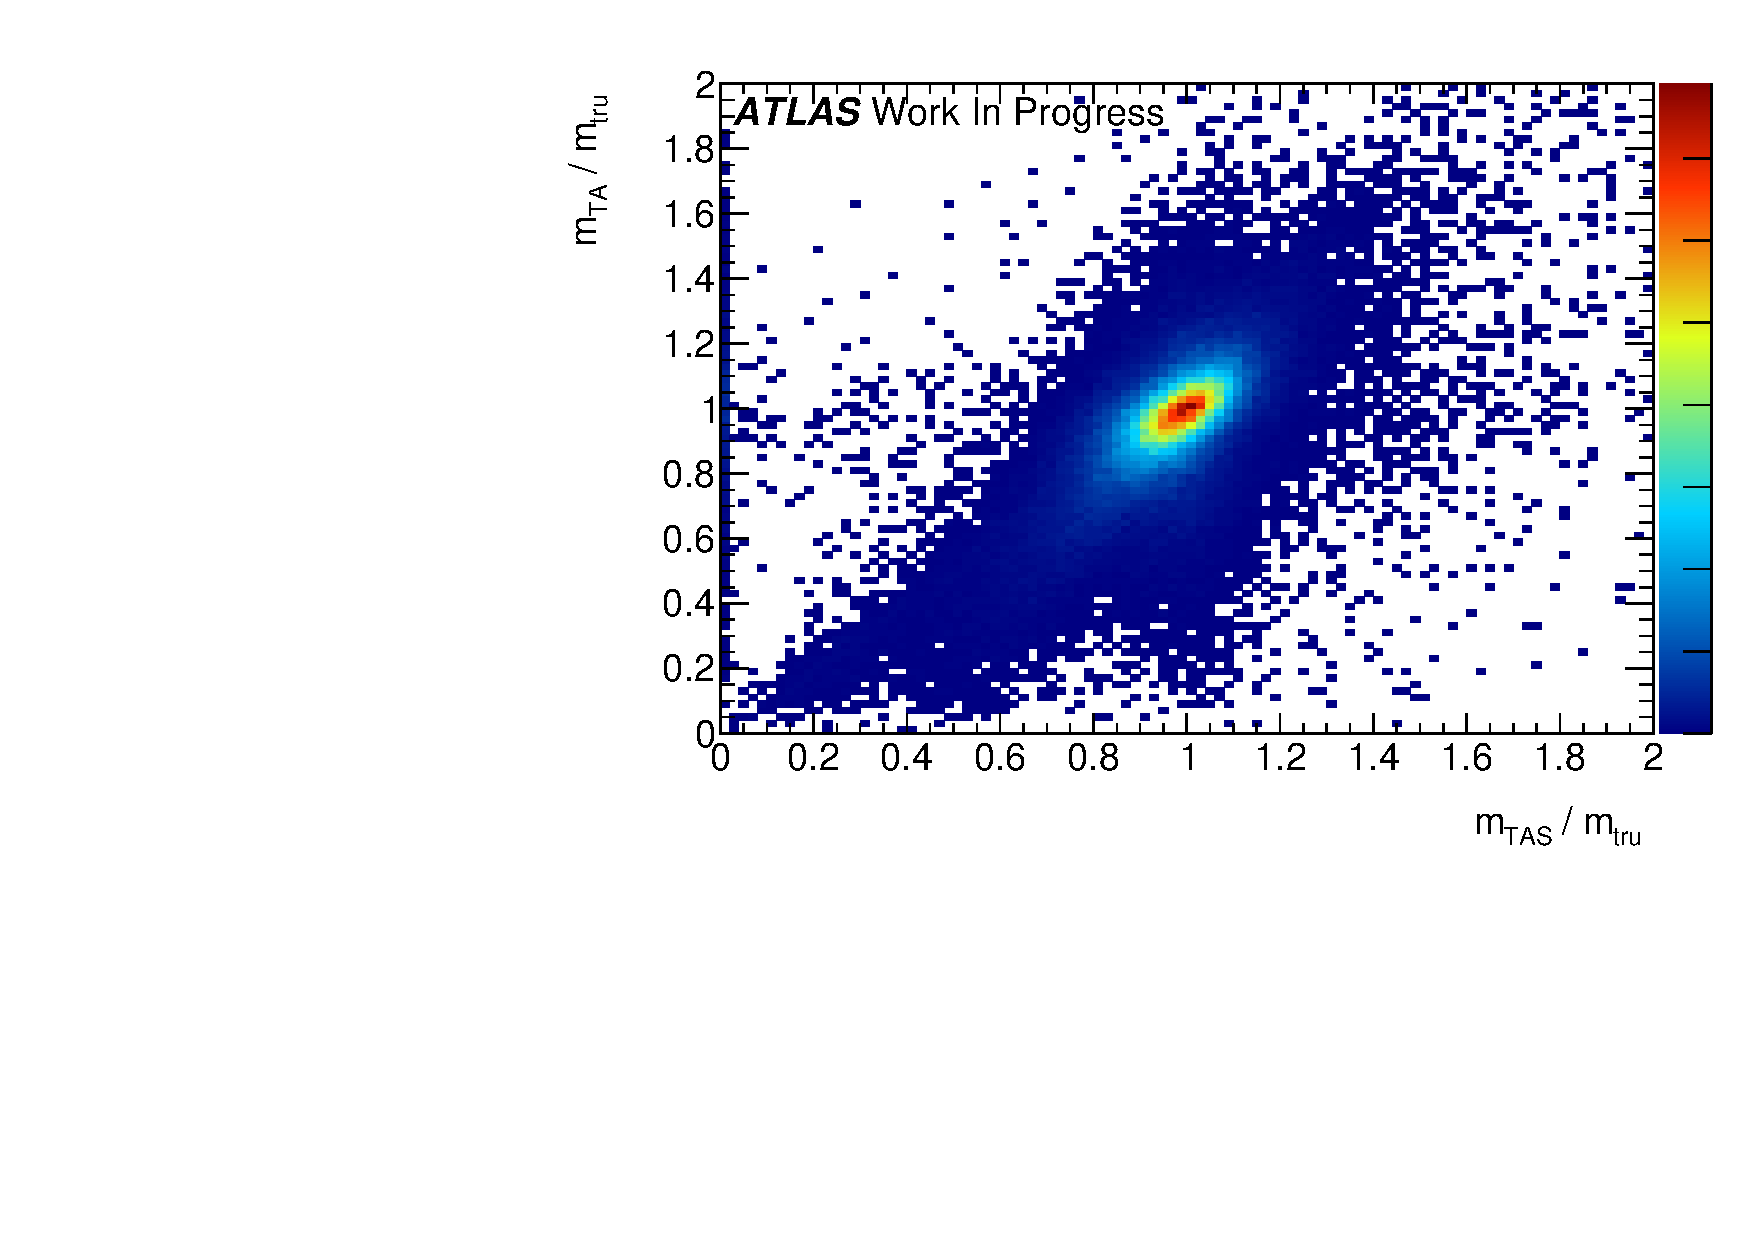
\includegraphics[width=0.4\textwidth]{/Users/fabnap/Documents/MasterArbeit/appendixB/mTAS_W_calibmCal_20:07:01-03-11-2016/1cfrt_h_fabsca_tasta_2.pdf}
\caption{Scatter plot $\mtas$ versus $\mta$ responses}
 
\end{figure}
 
\begin{figure}
 
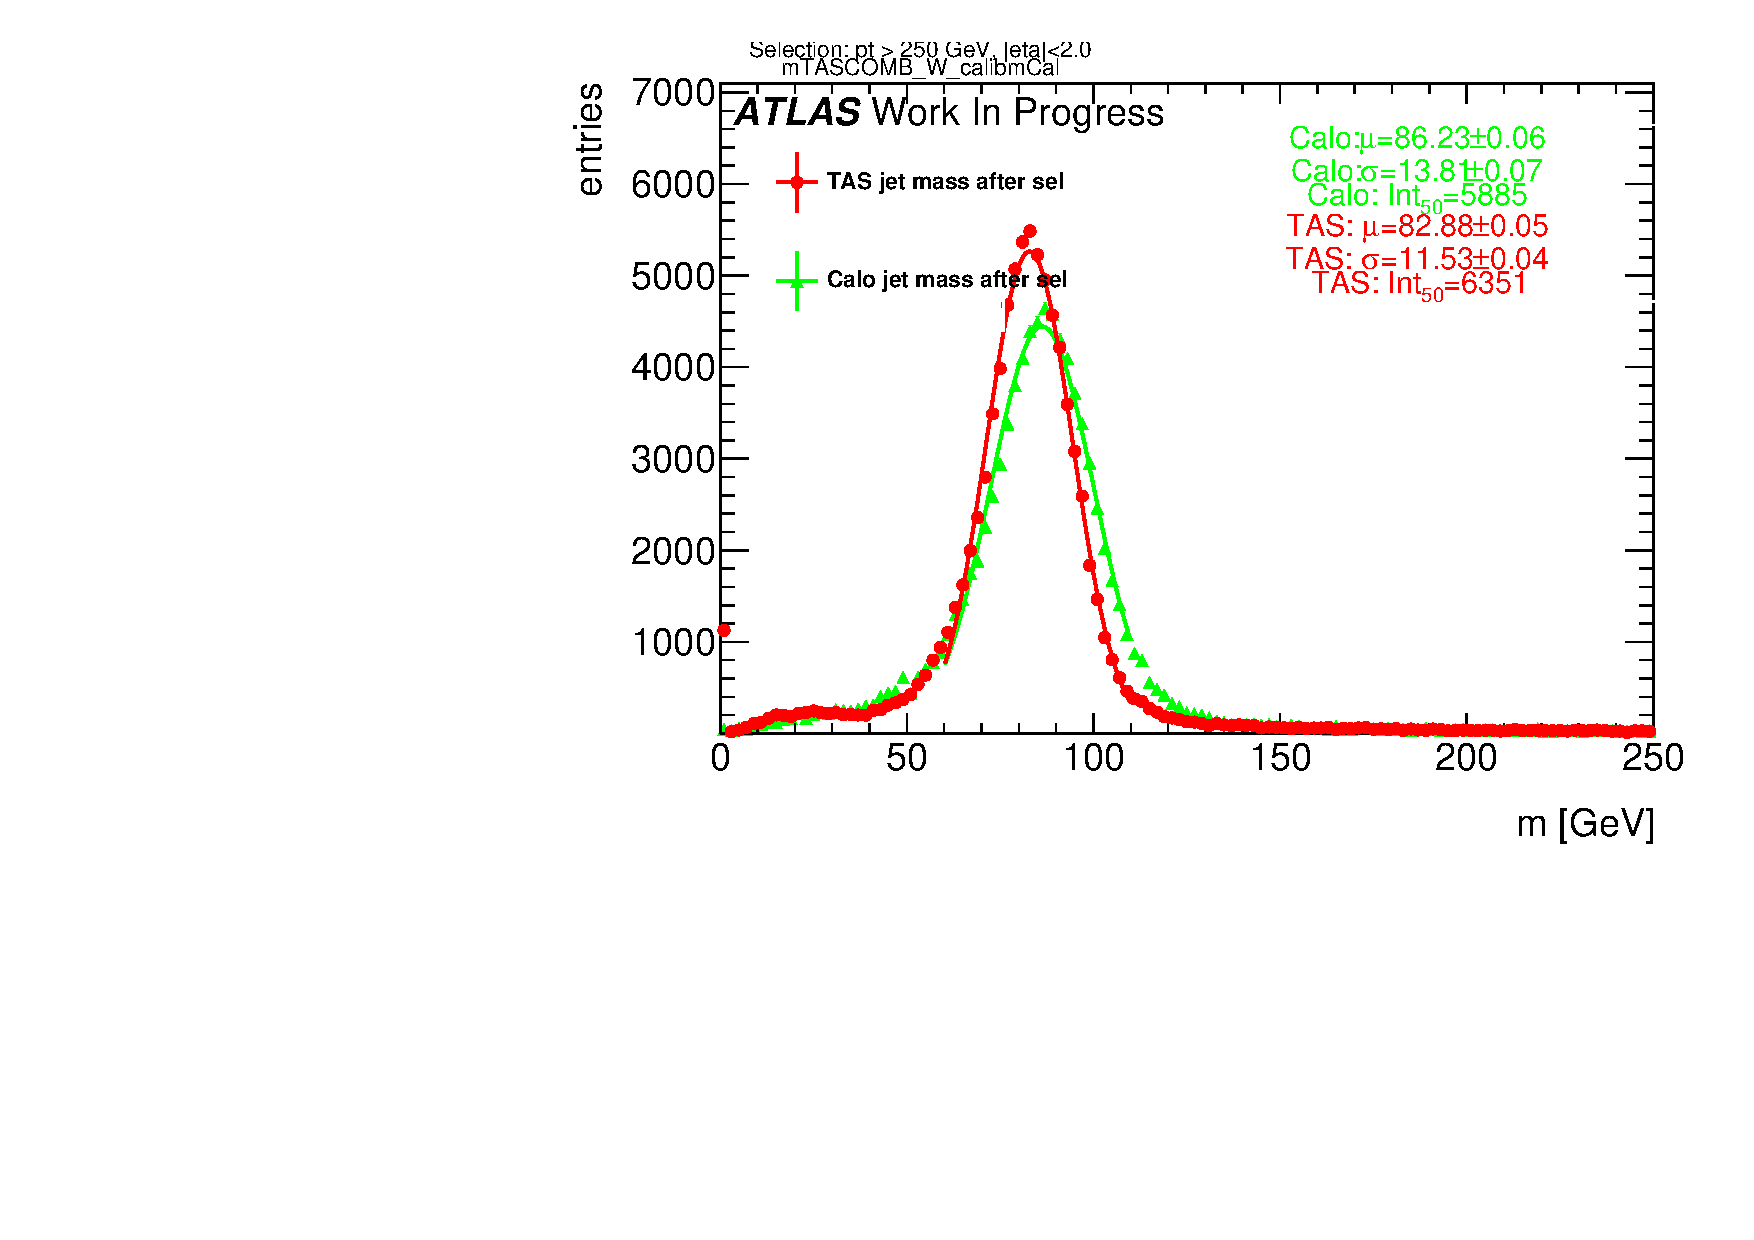
\includegraphics[width=0.4\textwidth]{/Users/fabnap/Documents/MasterArbeit/appendixB/mTAS_W_calibmCal_20:07:01-03-11-2016/1cfrt_h_FatJet_aftersel_m.pdf}
\caption{$\mtas$ distribution in all the $\pt$ bins}
 
\end{figure}
 
\begin{figure}
 
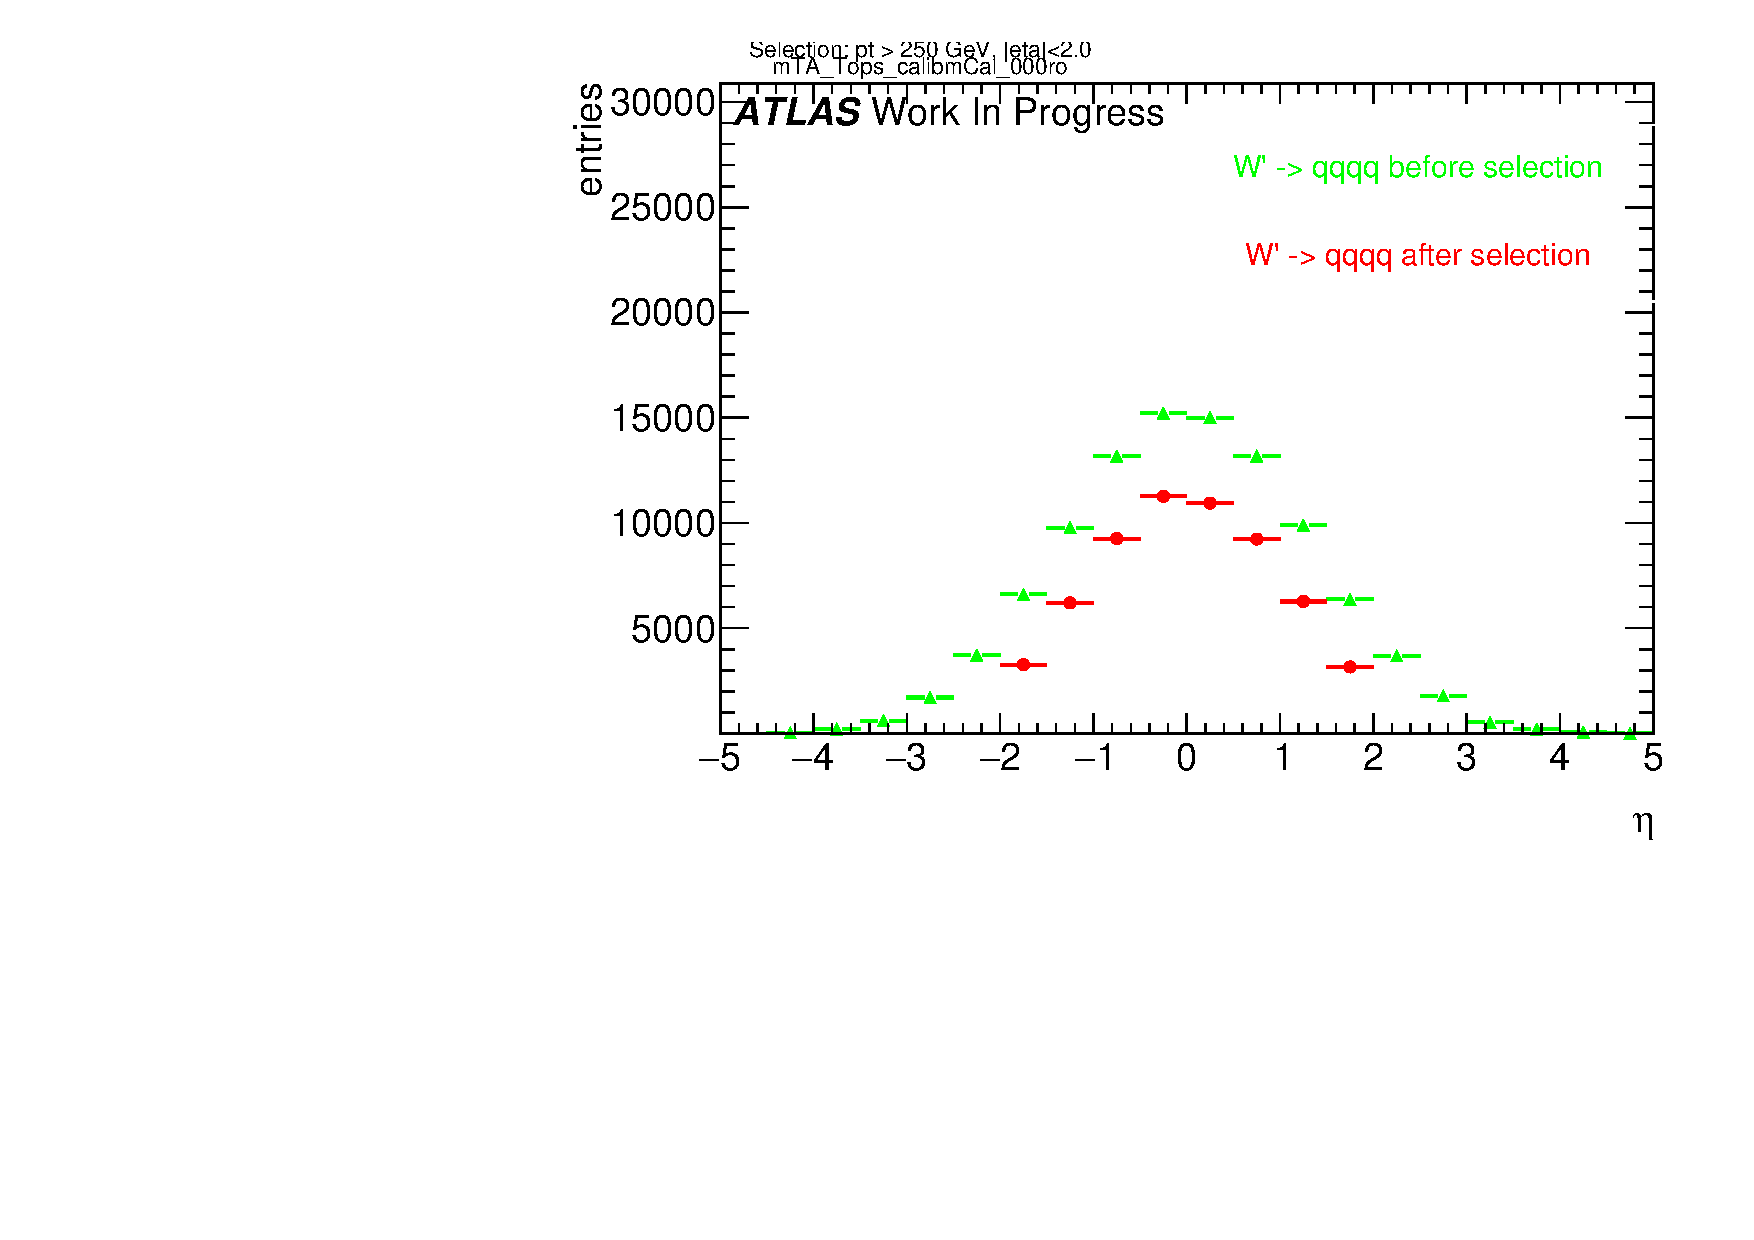
\includegraphics[width=0.4\textwidth]{/Users/fabnap/Documents/MasterArbeit/appendixB/mTAS_W_calibmCal_20:07:01-03-11-2016/1cfrt_h_FatJet_eta.pdf}
\caption{$\eta$ distribution of the large-R jet, before and after selection}
 
\end{figure}

\begin{figure}
 
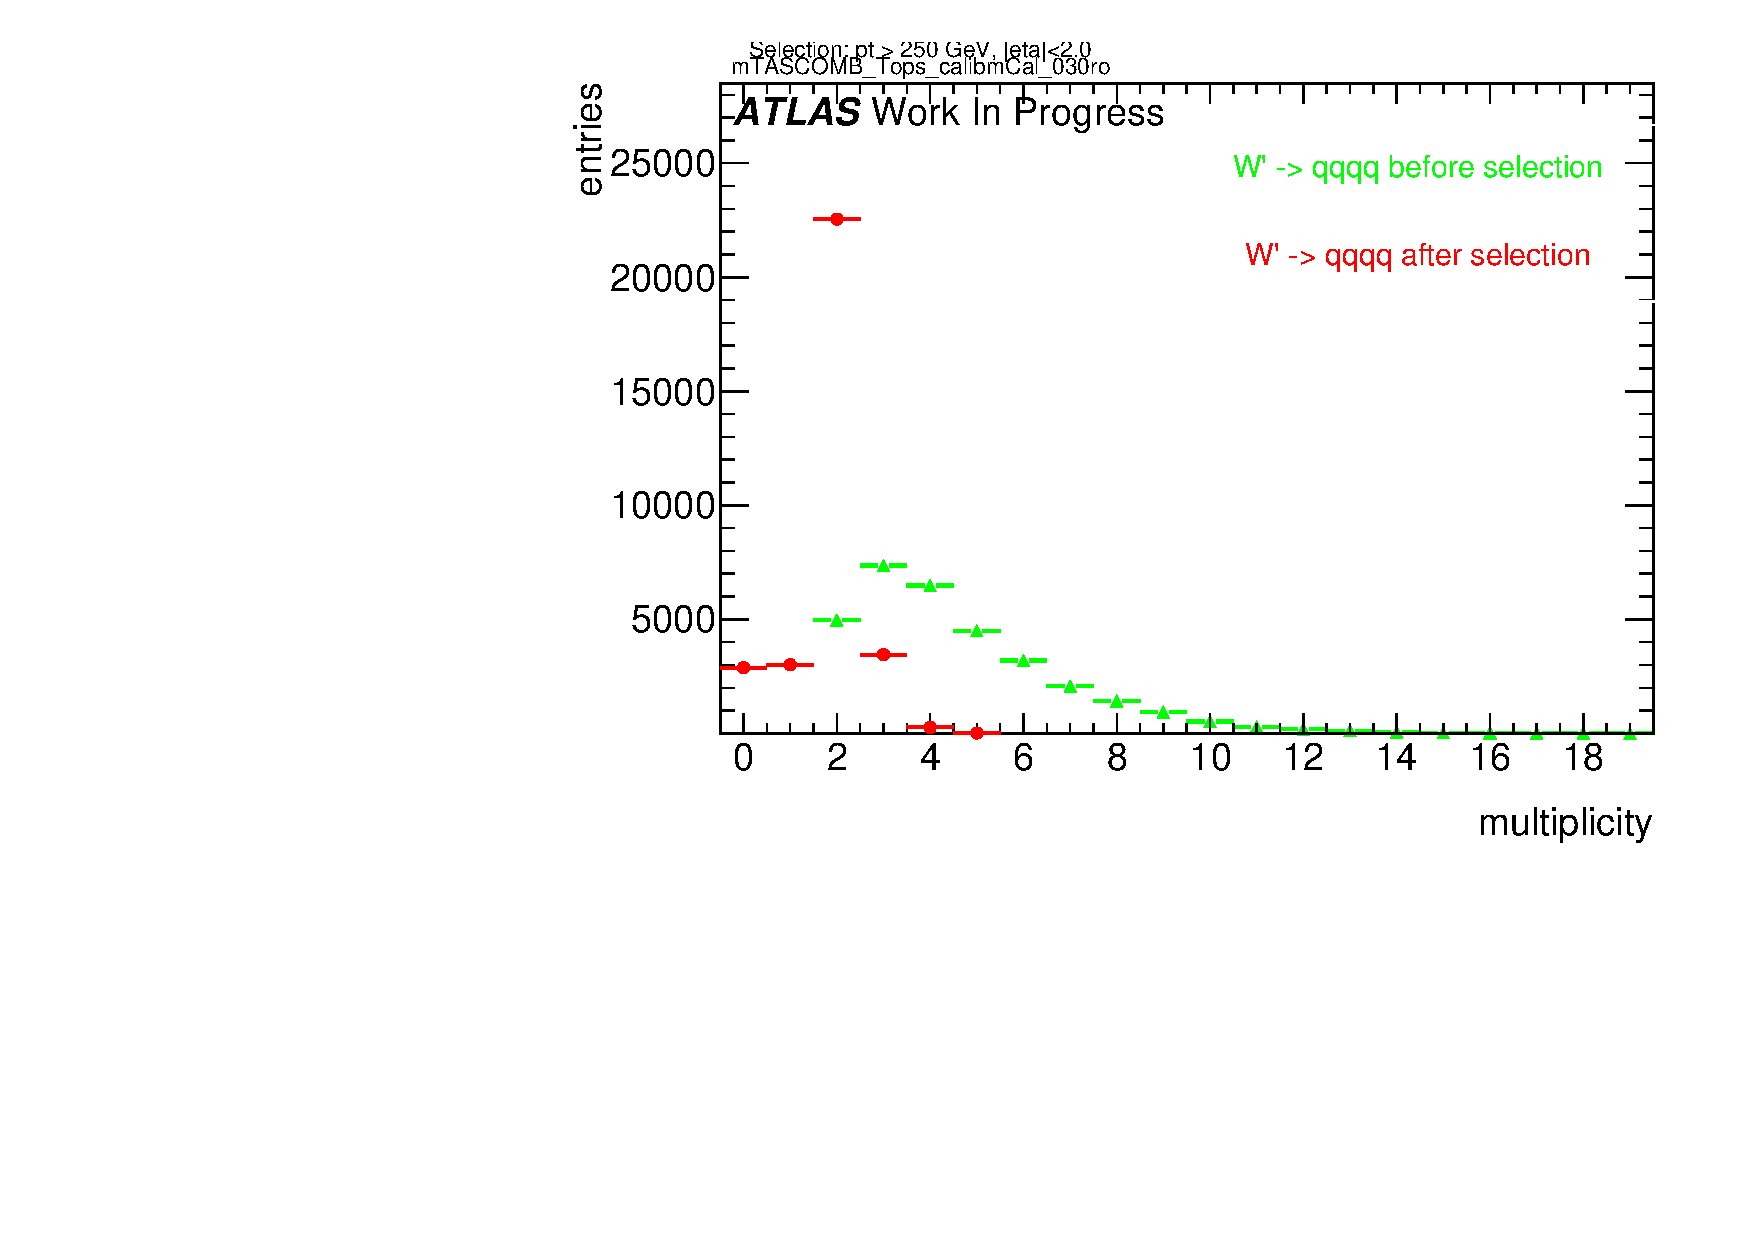
\includegraphics[width=0.4\textwidth]{/Users/fabnap/Documents/MasterArbeit/appendixB/mTAS_W_calibmCal_20:07:01-03-11-2016/1cfrt_h_FatJet_mult.pdf}
\caption{large-R jet Multiplicity, before and after selection}
 
\end{figure}
 
\begin{figure}
 
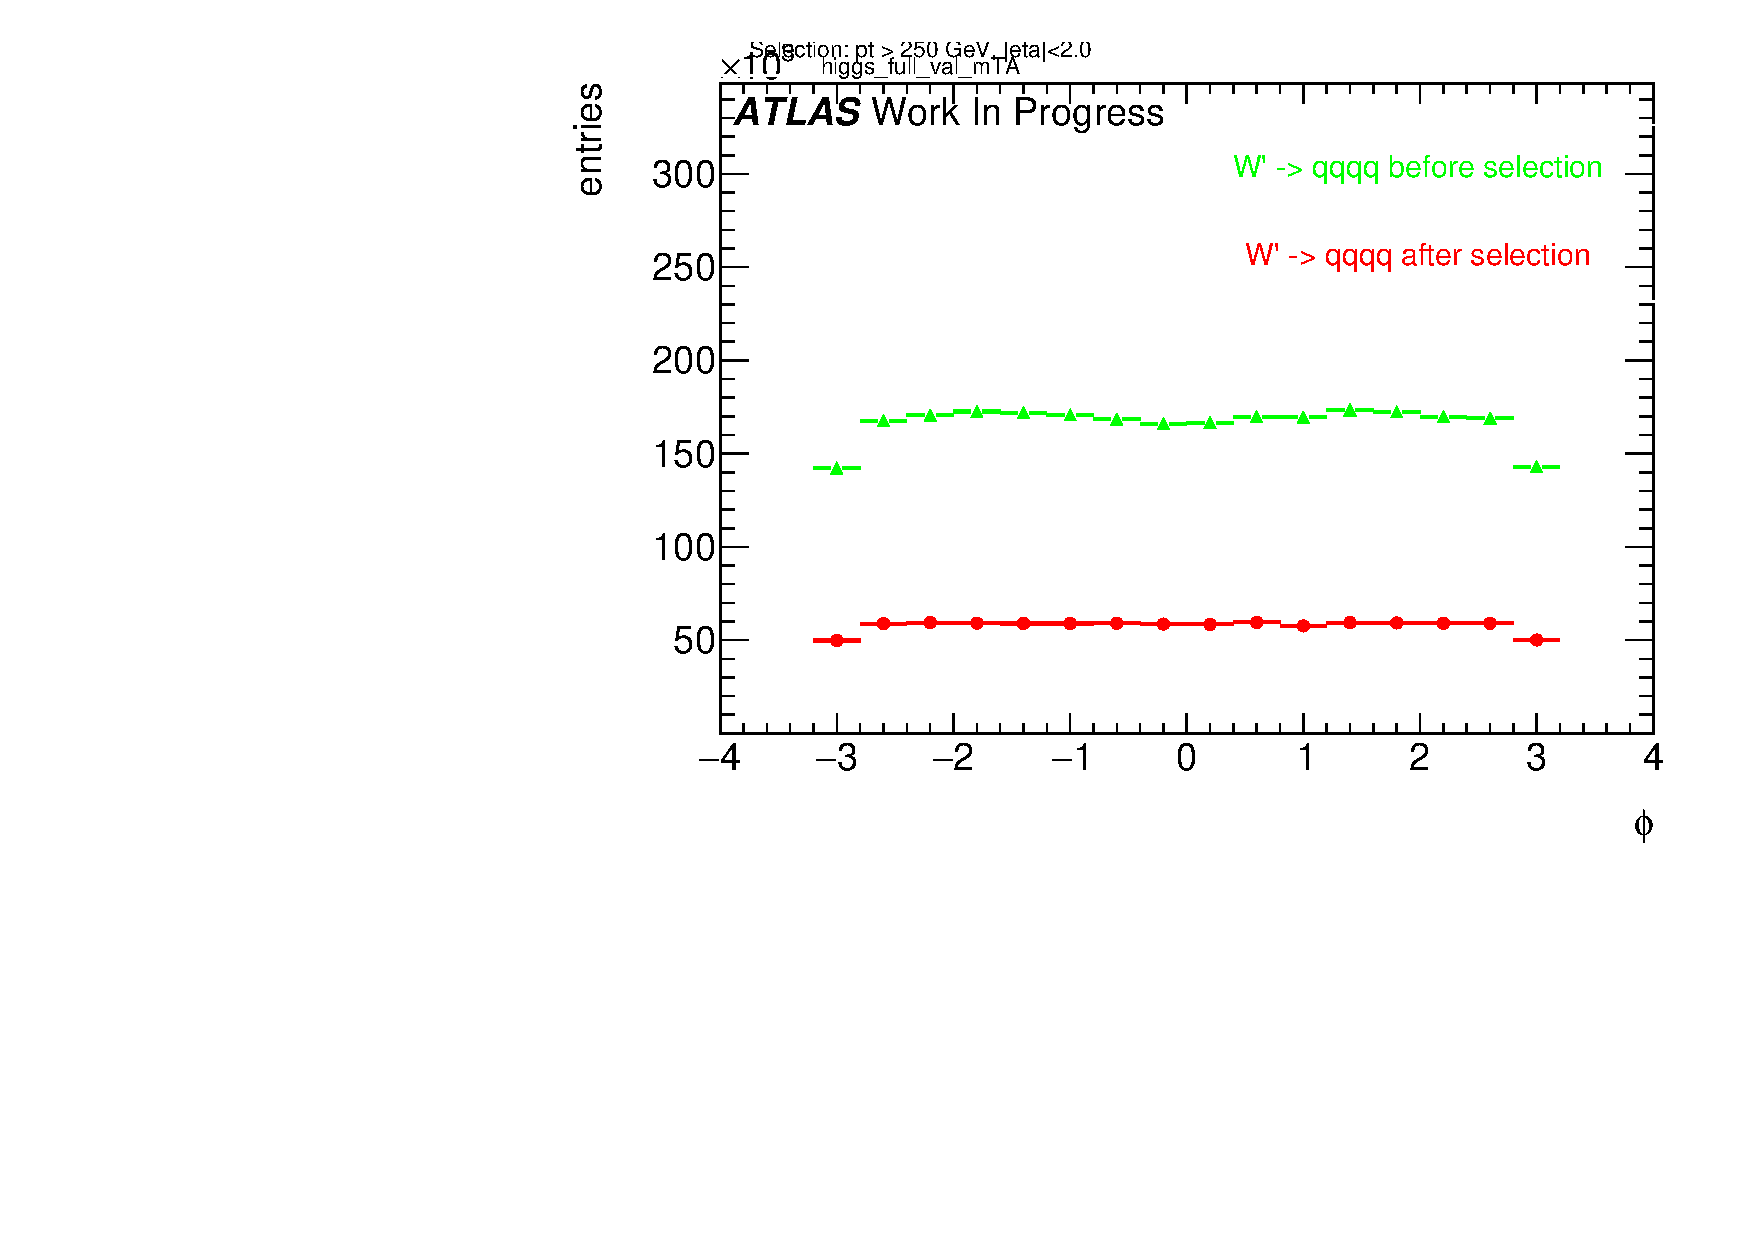
\includegraphics[width=0.4\textwidth]{/Users/fabnap/Documents/MasterArbeit/appendixB/mTAS_W_calibmCal_20:07:01-03-11-2016/1cfrt_h_FatJet_psi.pdf}
\caption{$\phi$ distribution of the large-R jet, before and after selection}
 
\end{figure}
 
\begin{figure}
 
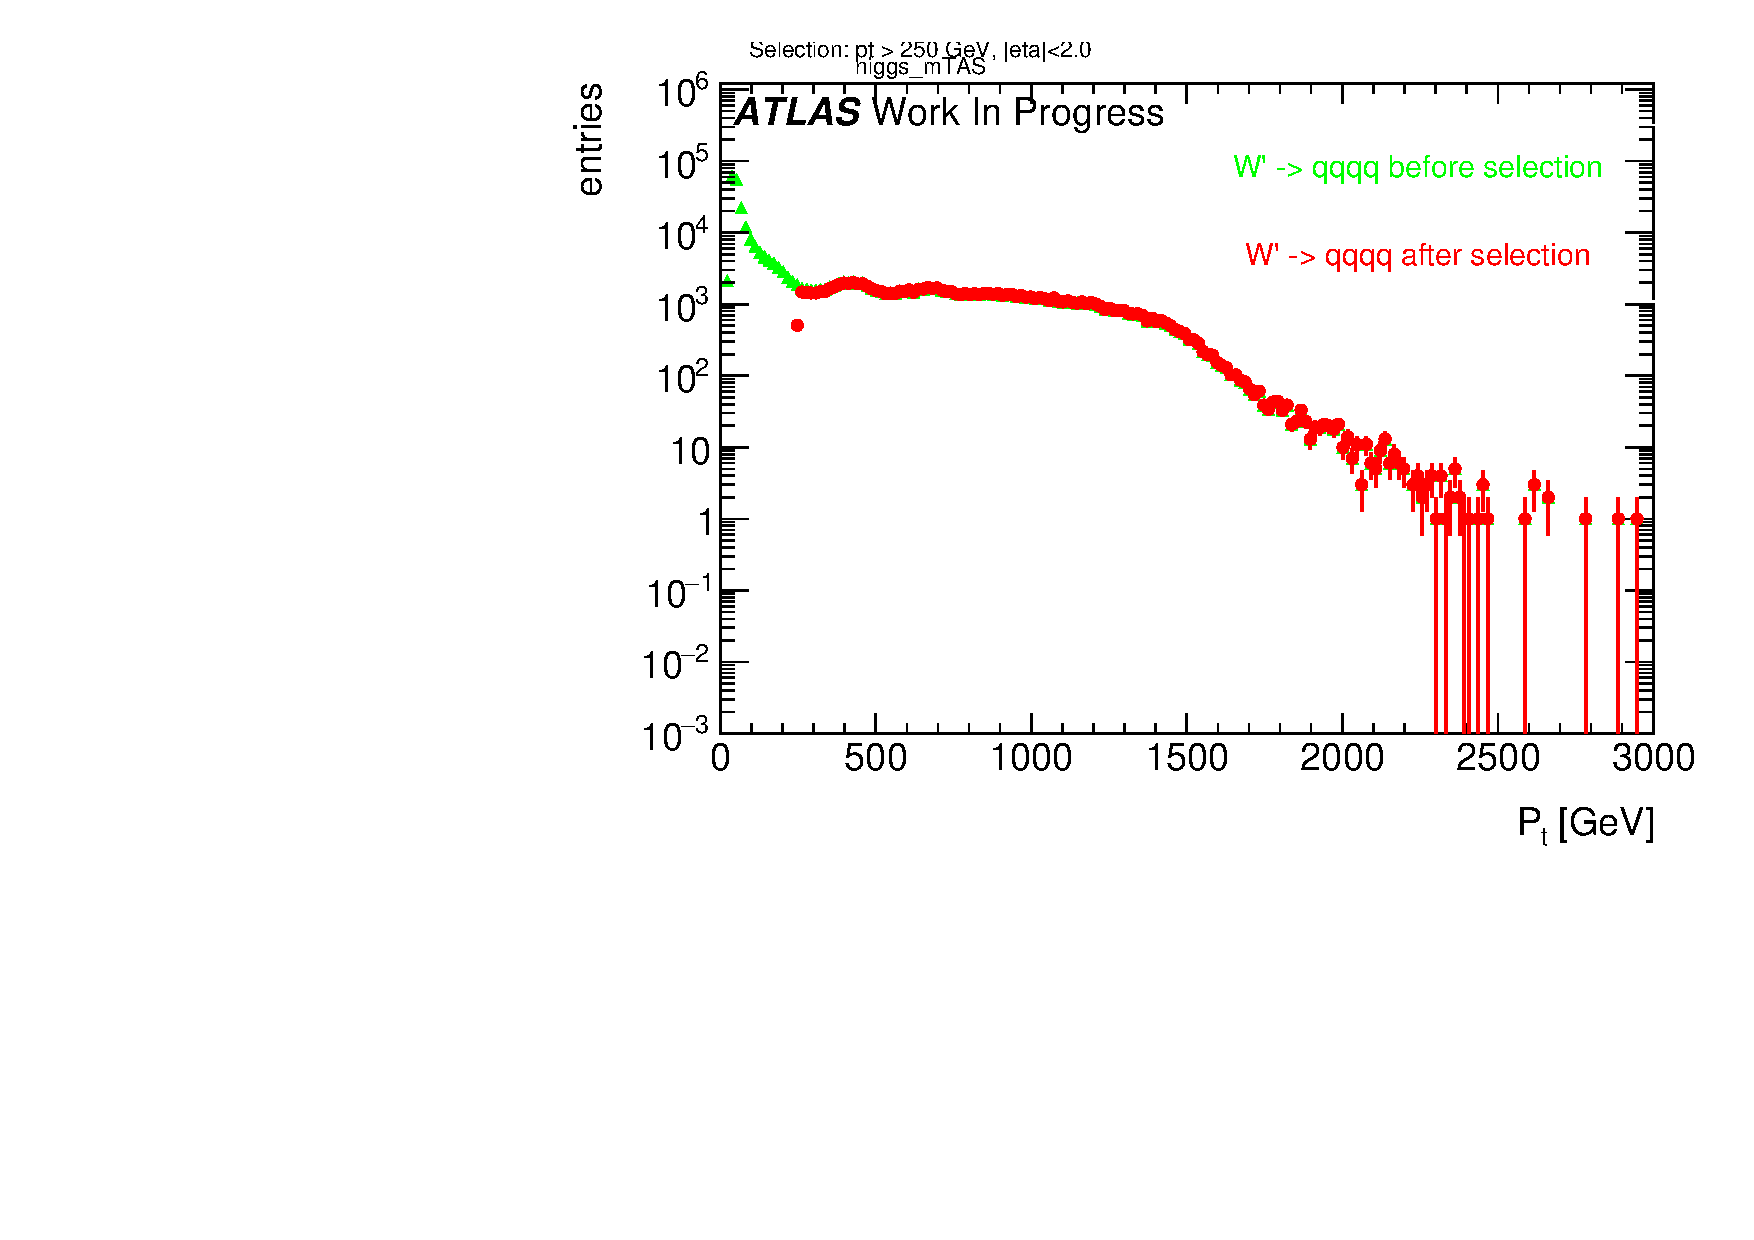
\includegraphics[width=0.4\textwidth]{/Users/fabnap/Documents/MasterArbeit/appendixB/mTAS_W_calibmCal_20:07:01-03-11-2016/1cfrt_h_FatJet_pt.pdf}
\caption{$p_{T}$ distribution of the large-R jet, before and after selection}
 
\end{figure}
 
\begin{figure}
 
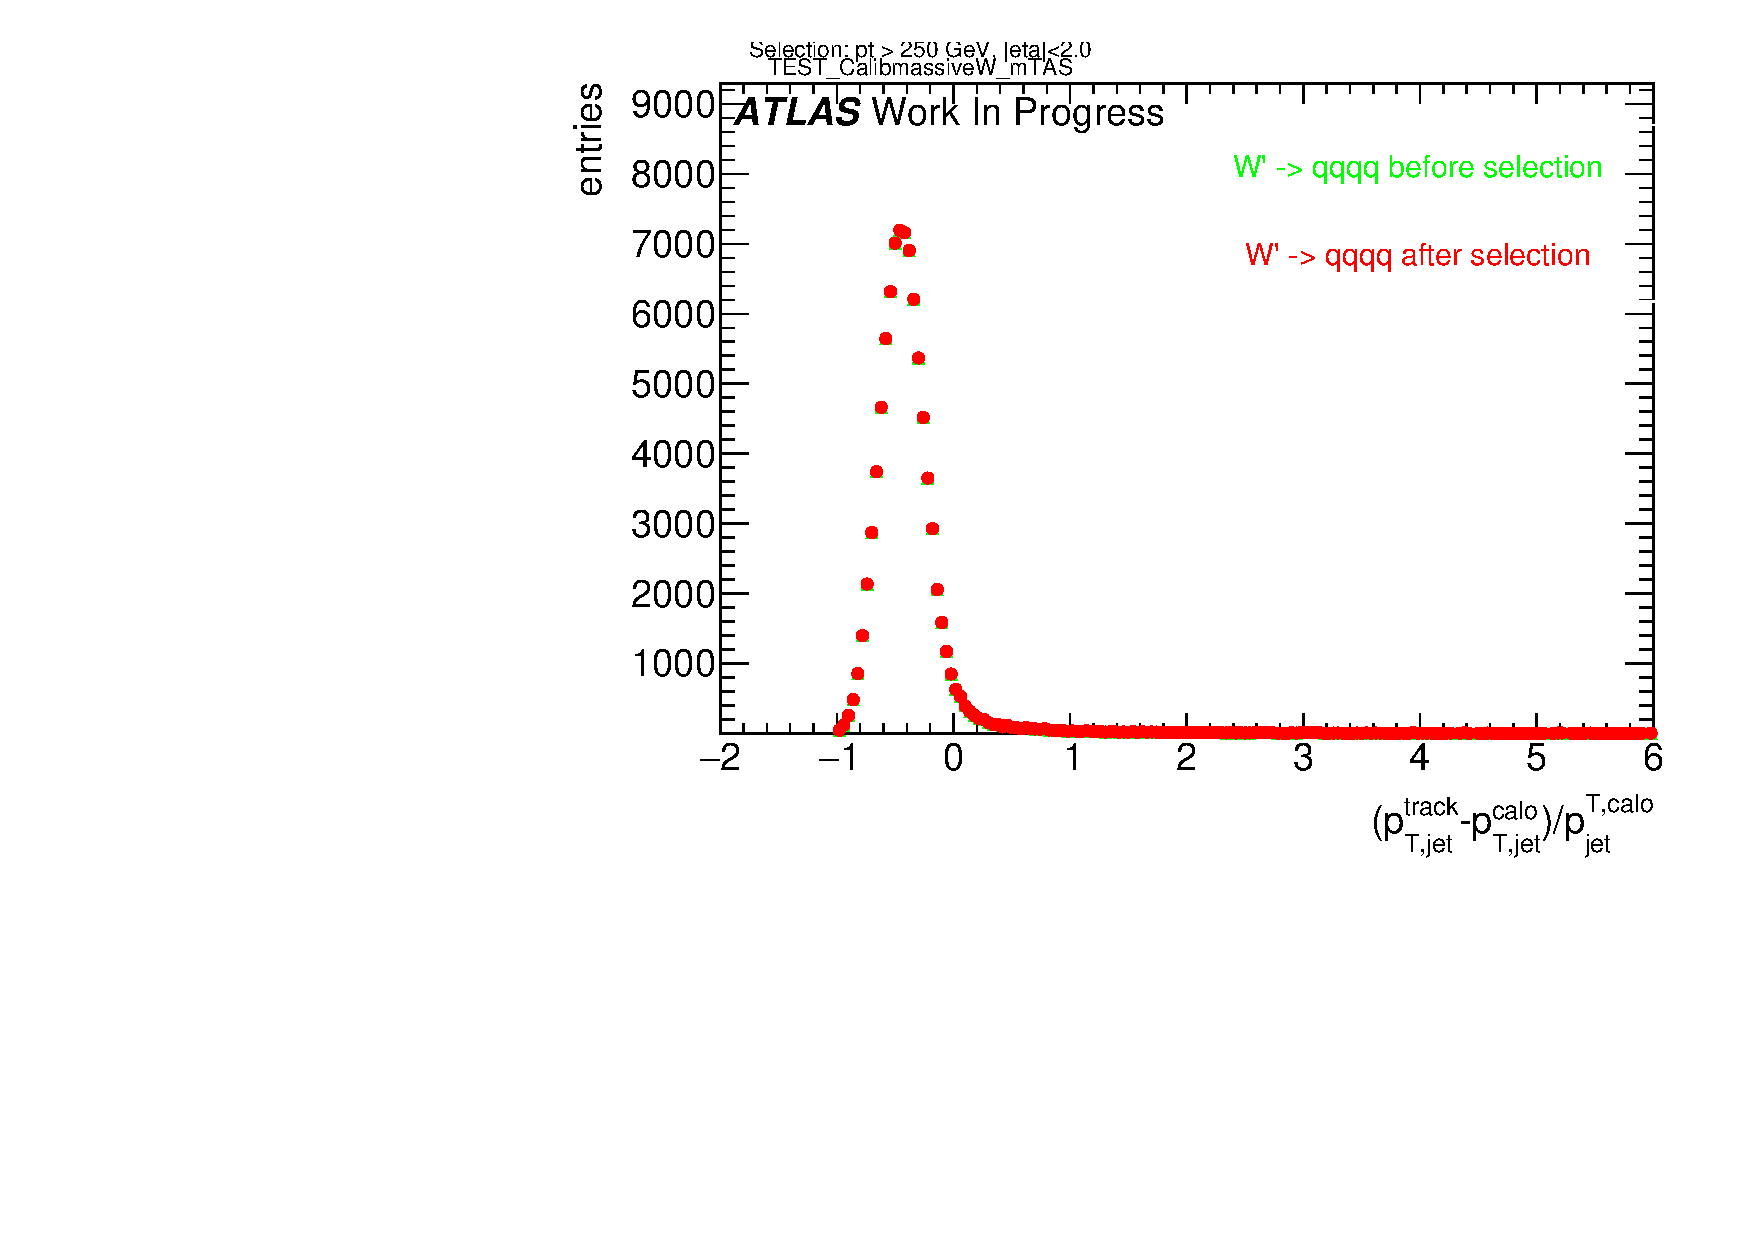
\includegraphics[width=0.4\textwidth]{/Users/fabnap/Documents/MasterArbeit/appendixB/mTAS_W_calibmCal_20:07:01-03-11-2016/1cfrt_h_FatJet_ptres.pdf}
\caption{$\pt$ resolution: $\frac{p_{T,jet}^{track}-p_{T,jet}^{fat}}{p_{T,jet}^{fat}}$, before and after selection }
 
\end{figure}
 
\begin{figure}
 
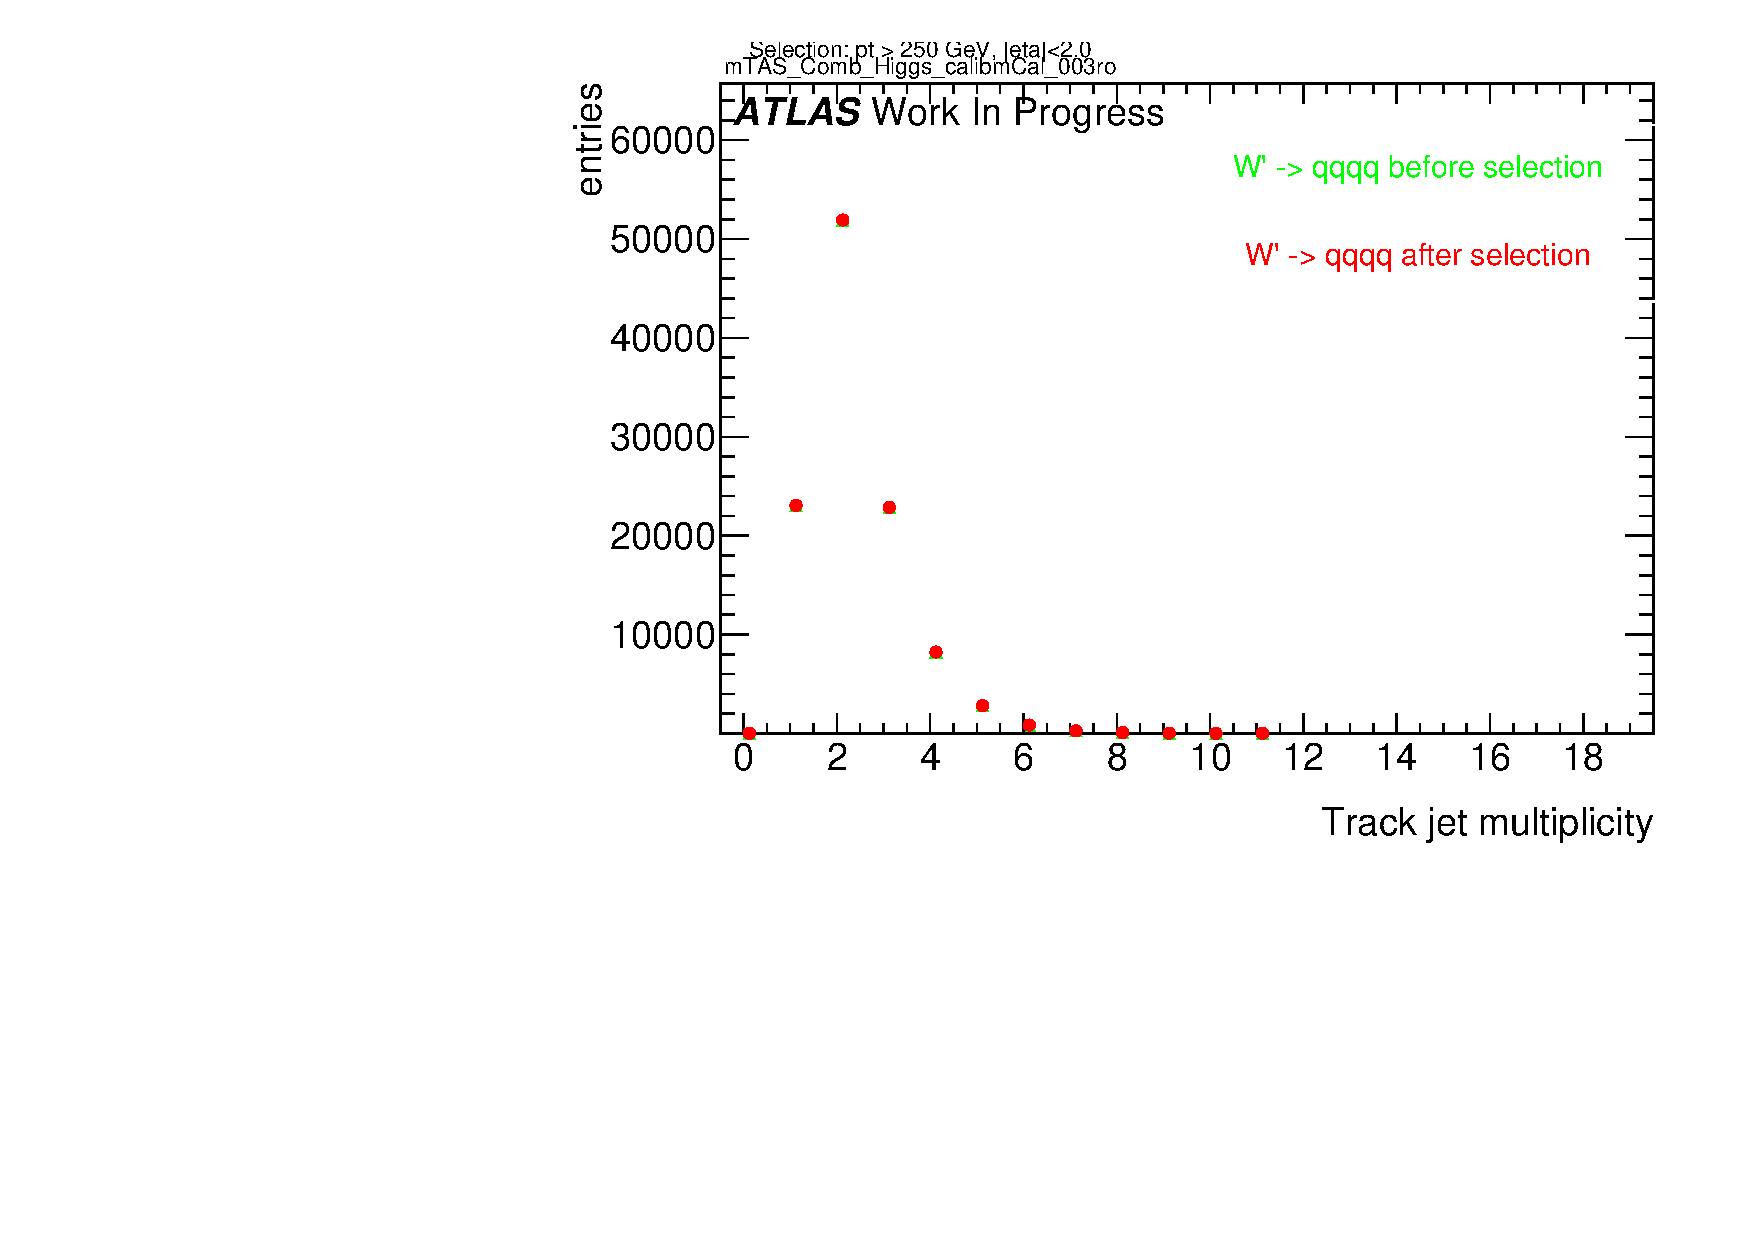
\includegraphics[width=0.4\textwidth]{/Users/fabnap/Documents/MasterArbeit/appendixB/mTAS_W_calibmCal_20:07:01-03-11-2016/1cfrt_h_FatJet_TAmult.pdf}
\caption{Multiplicity of track-jets R=0.2 per large-R jet}
 
\end{figure}
 %
\begin{figure}
 
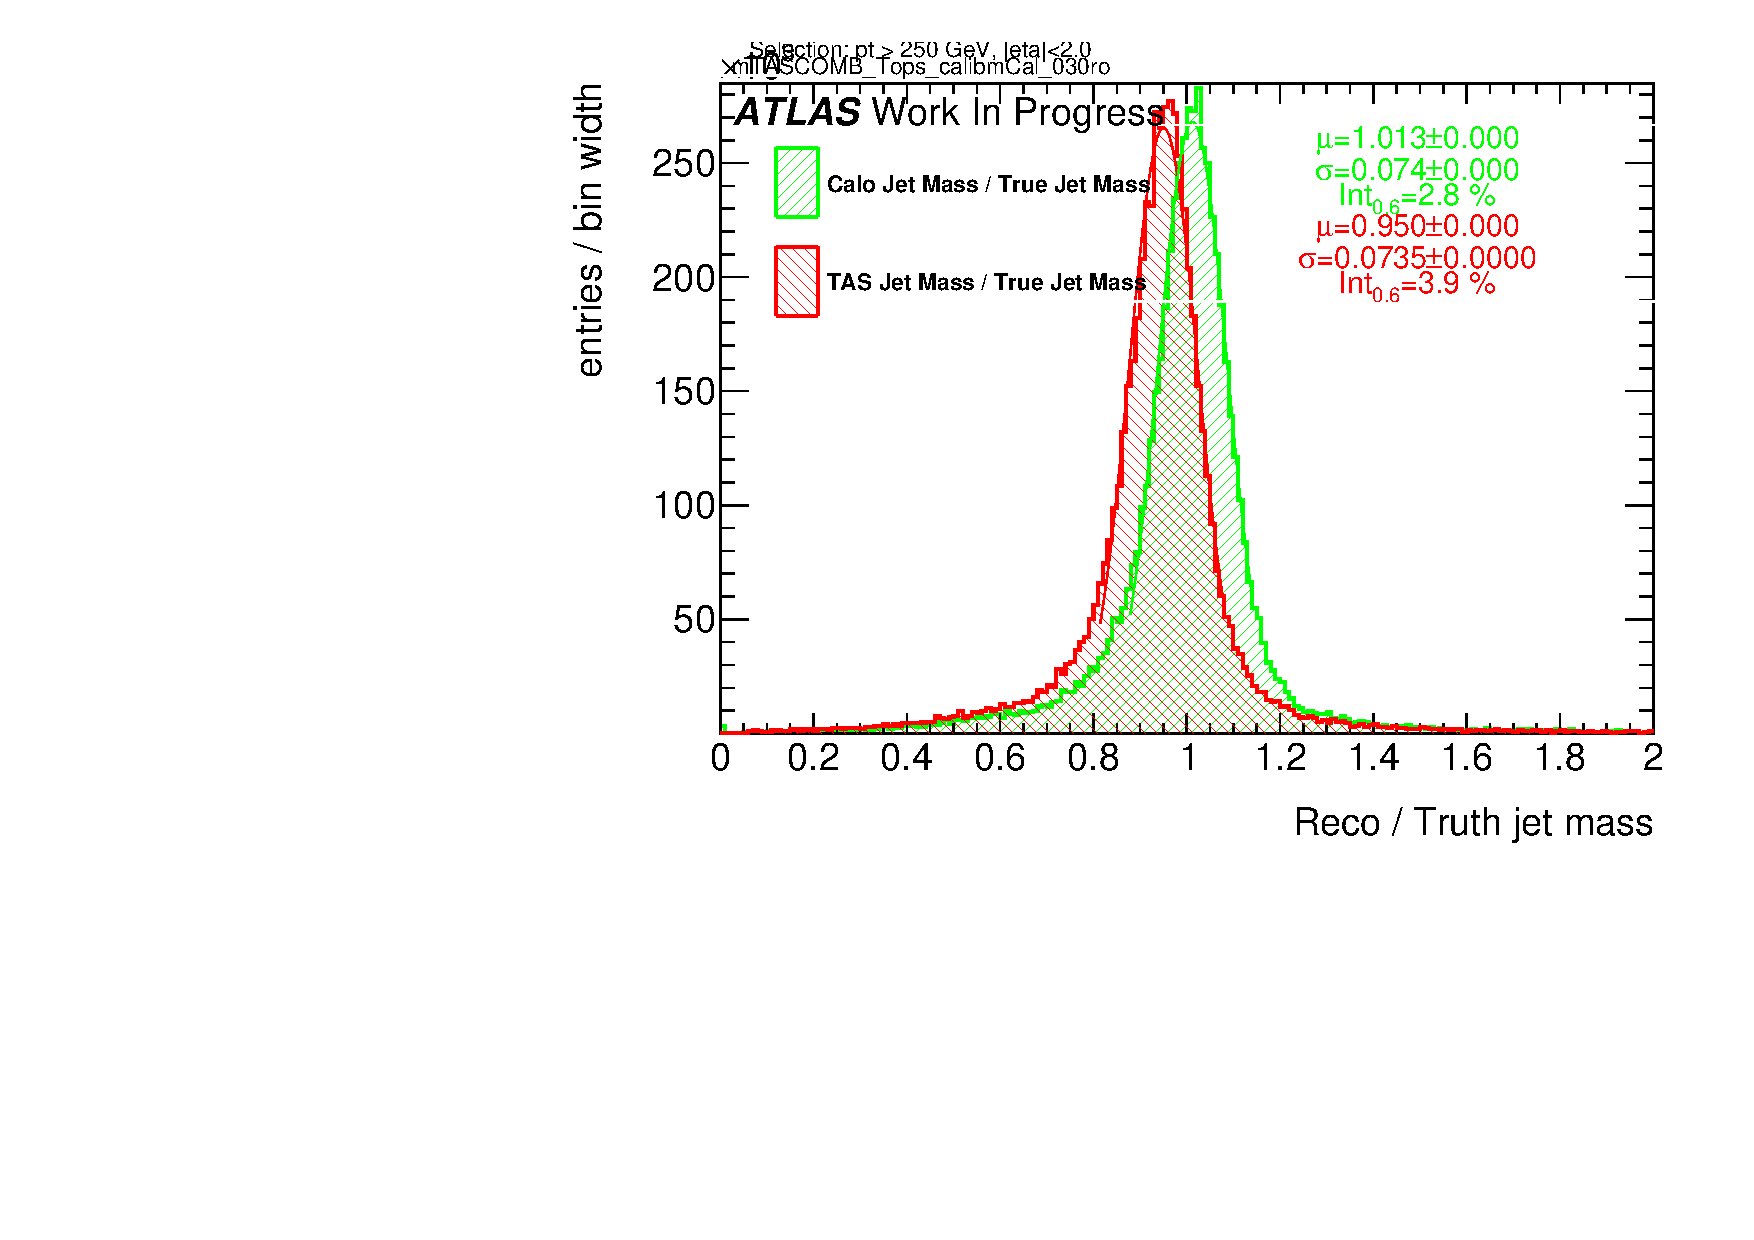
\includegraphics[width=0.4\textwidth]{/Users/fabnap/Documents/MasterArbeit/appendixB/mTAS_W_calibmCal_20:07:01-03-11-2016/1cfrt_h_JetRatio_m.pdf}
\caption{Response $m^{Reco} / m^{Truth}$ for all the $\pt$ bins}
 
\end{figure}
 
\begin{figure}
 
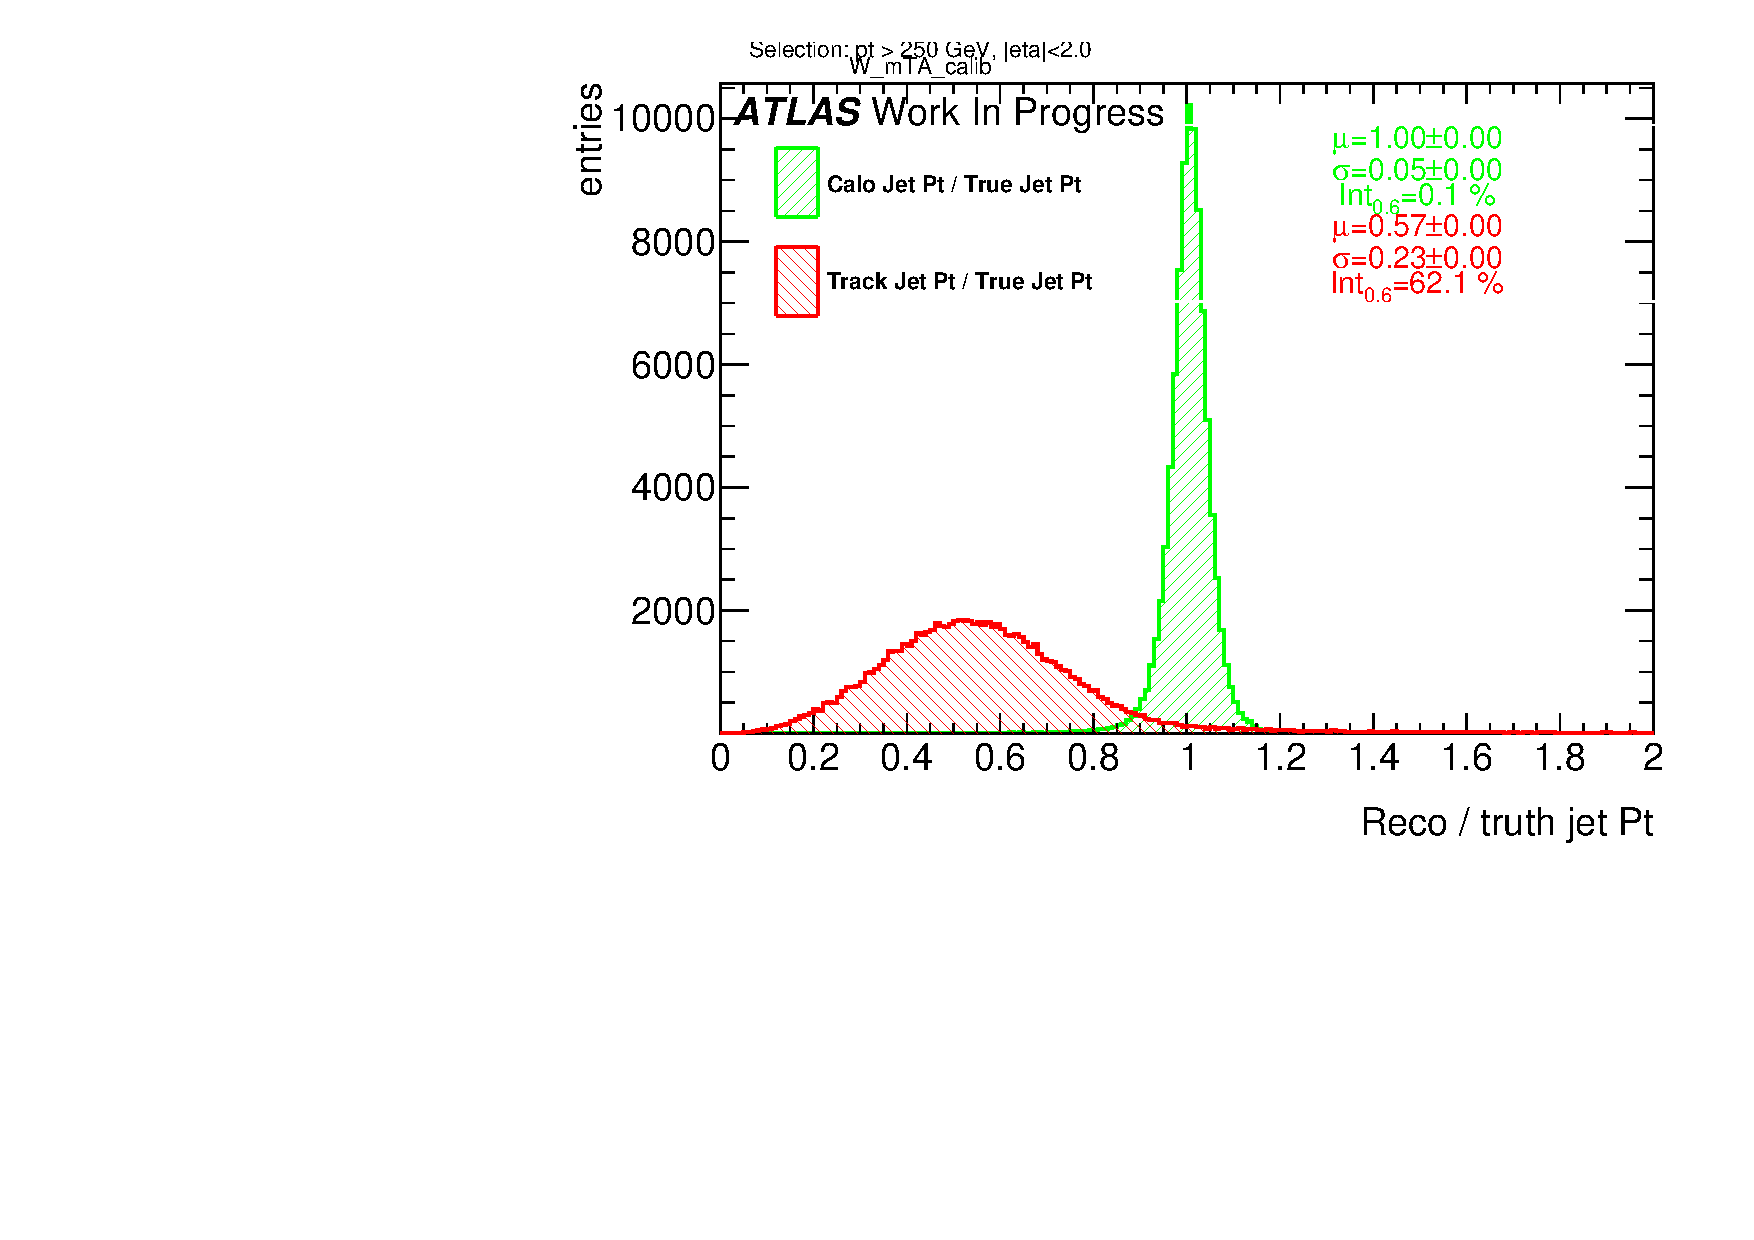
\includegraphics[width=0.4\textwidth]{/Users/fabnap/Documents/MasterArbeit/appendixB/mTAS_W_calibmCal_20:07:01-03-11-2016/1cfrt_h_JetRatio_pt.pdf}
\caption{Transverse momentum response $p_{T}^{Reco} / p_{T}^{Truth}$ for calorimeter and tracks}
 
\end{figure}
 
\begin{figure}
 
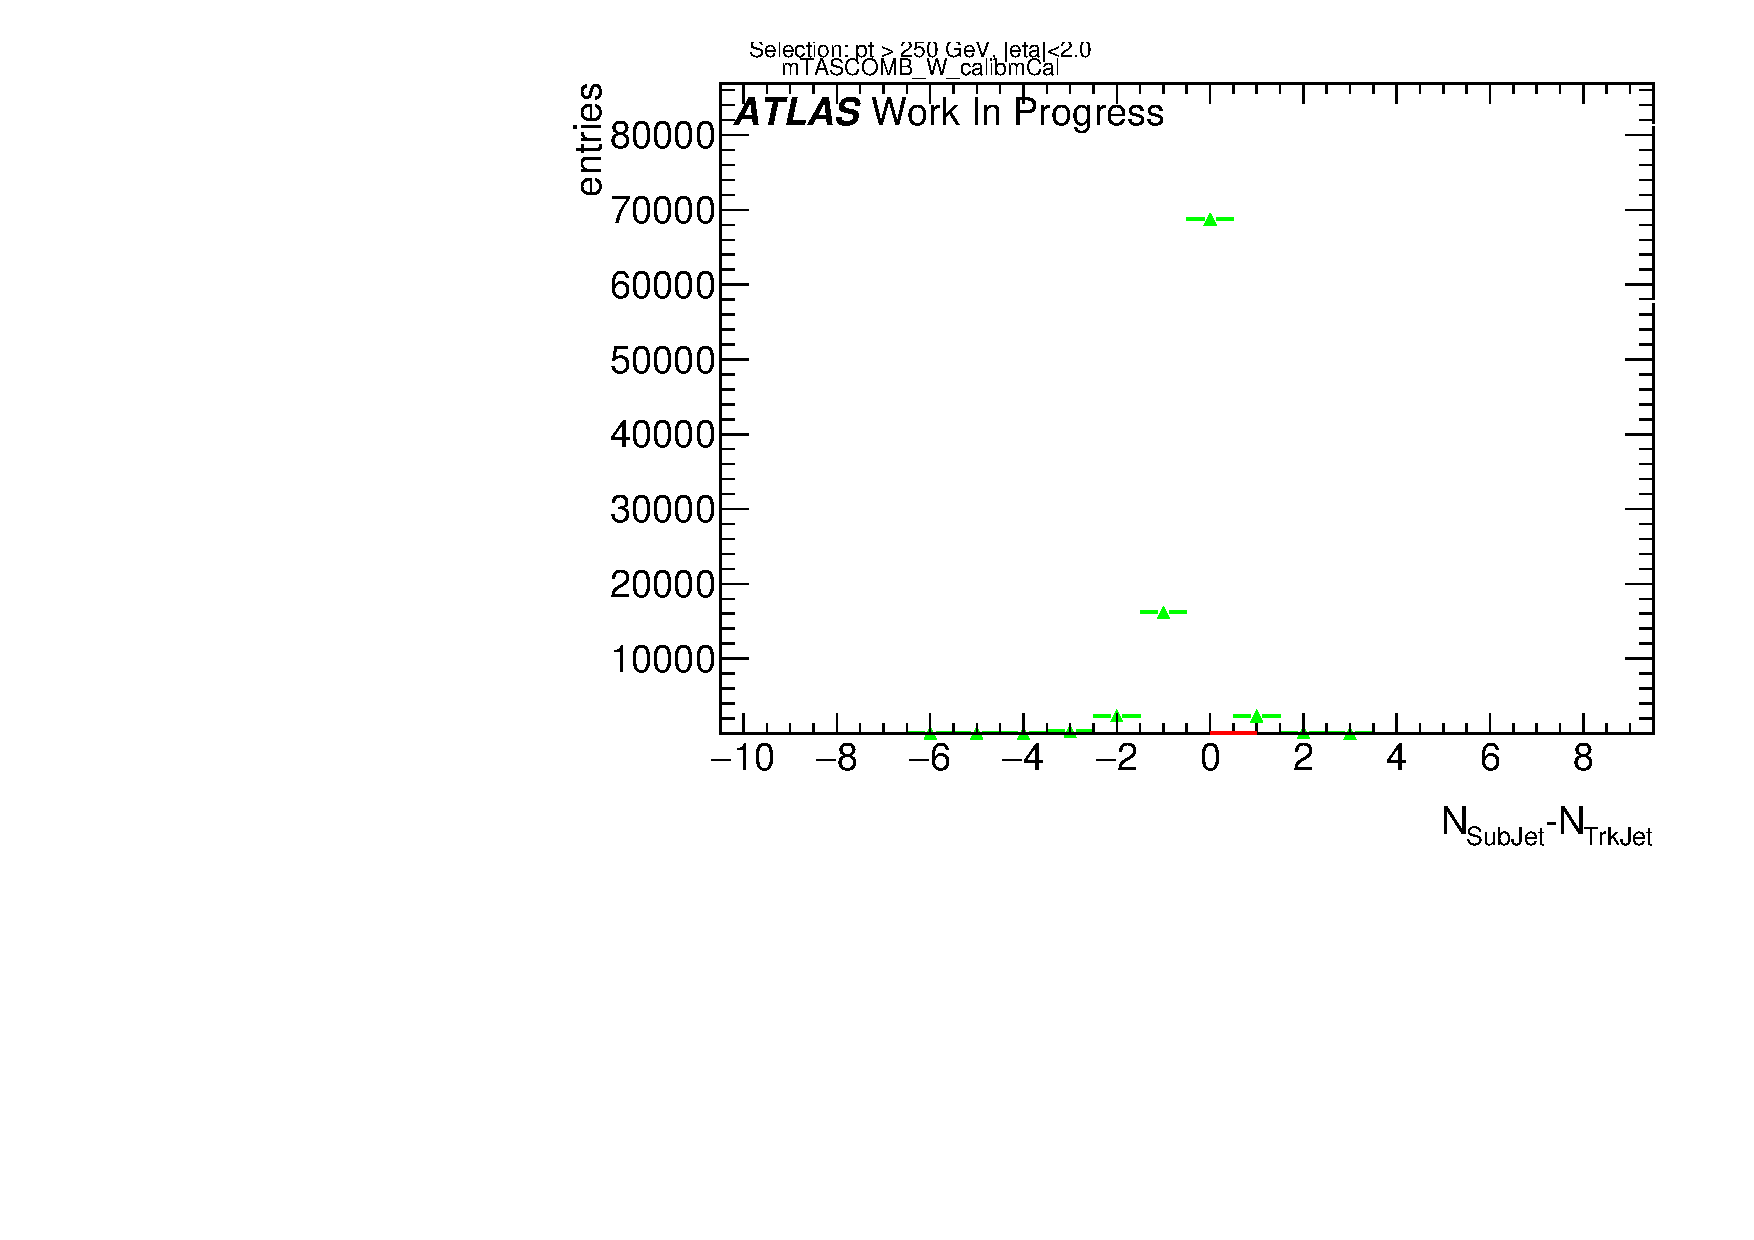
\includegraphics[width=0.4\textwidth]{/Users/fabnap/Documents/MasterArbeit/appendixB/mTAS_W_calibmCal_20:07:01-03-11-2016/1cfrt_h_NfminusNi.pdf}
\caption{sub-jet - track-jet Multiplicity}
 
\end{figure}

\clearpage

\begin{figure}
 
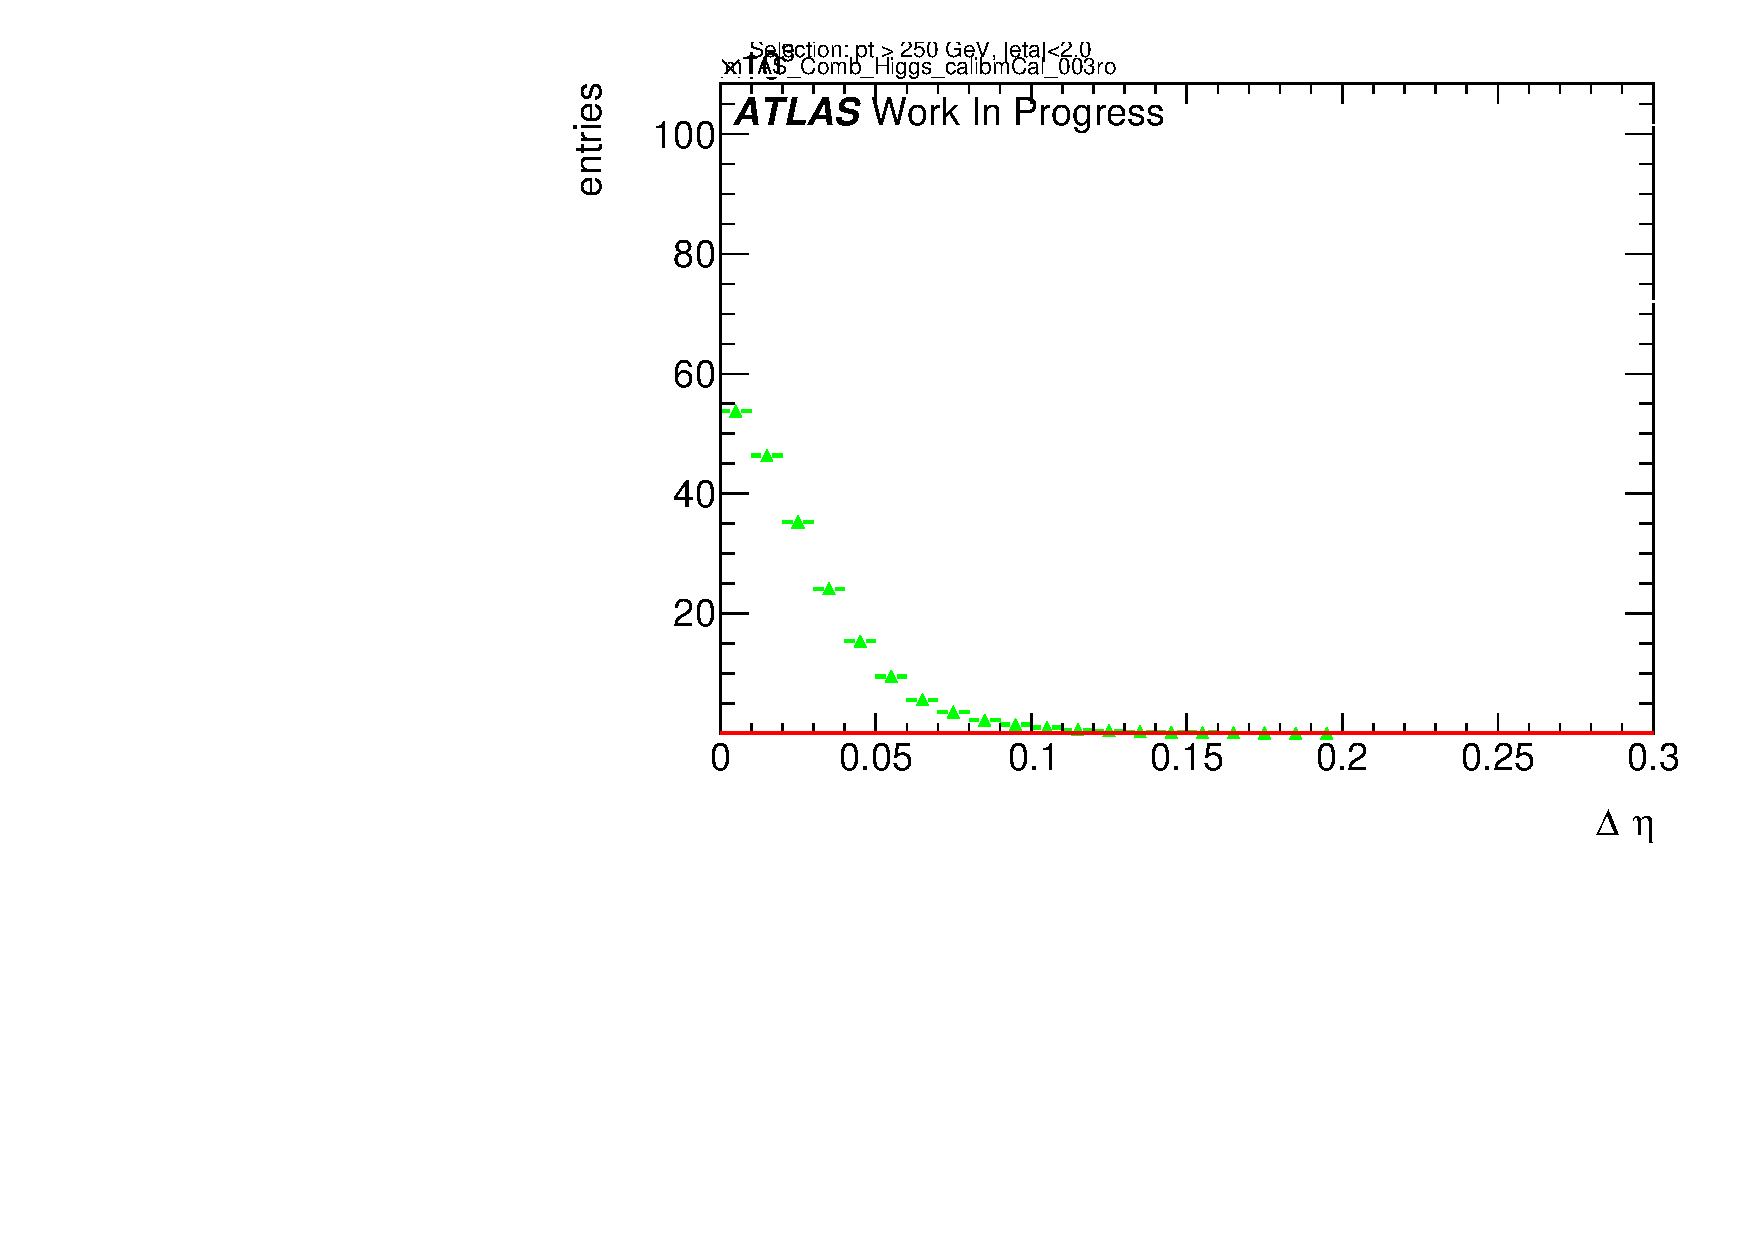
\includegraphics[width=0.4\textwidth]{/Users/fabnap/Documents/MasterArbeit/appendixB/mTAS_W_calibmCal_20:07:01-03-11-2016/1cfrt_h_SubJet_Delta_eta.pdf}
\caption{$| \eta_{sub-jet} - \eta_{track-jet} | $ distribution, where sub-jet and track-jet are the closest}
 
\end{figure}
 
\begin{figure}
 
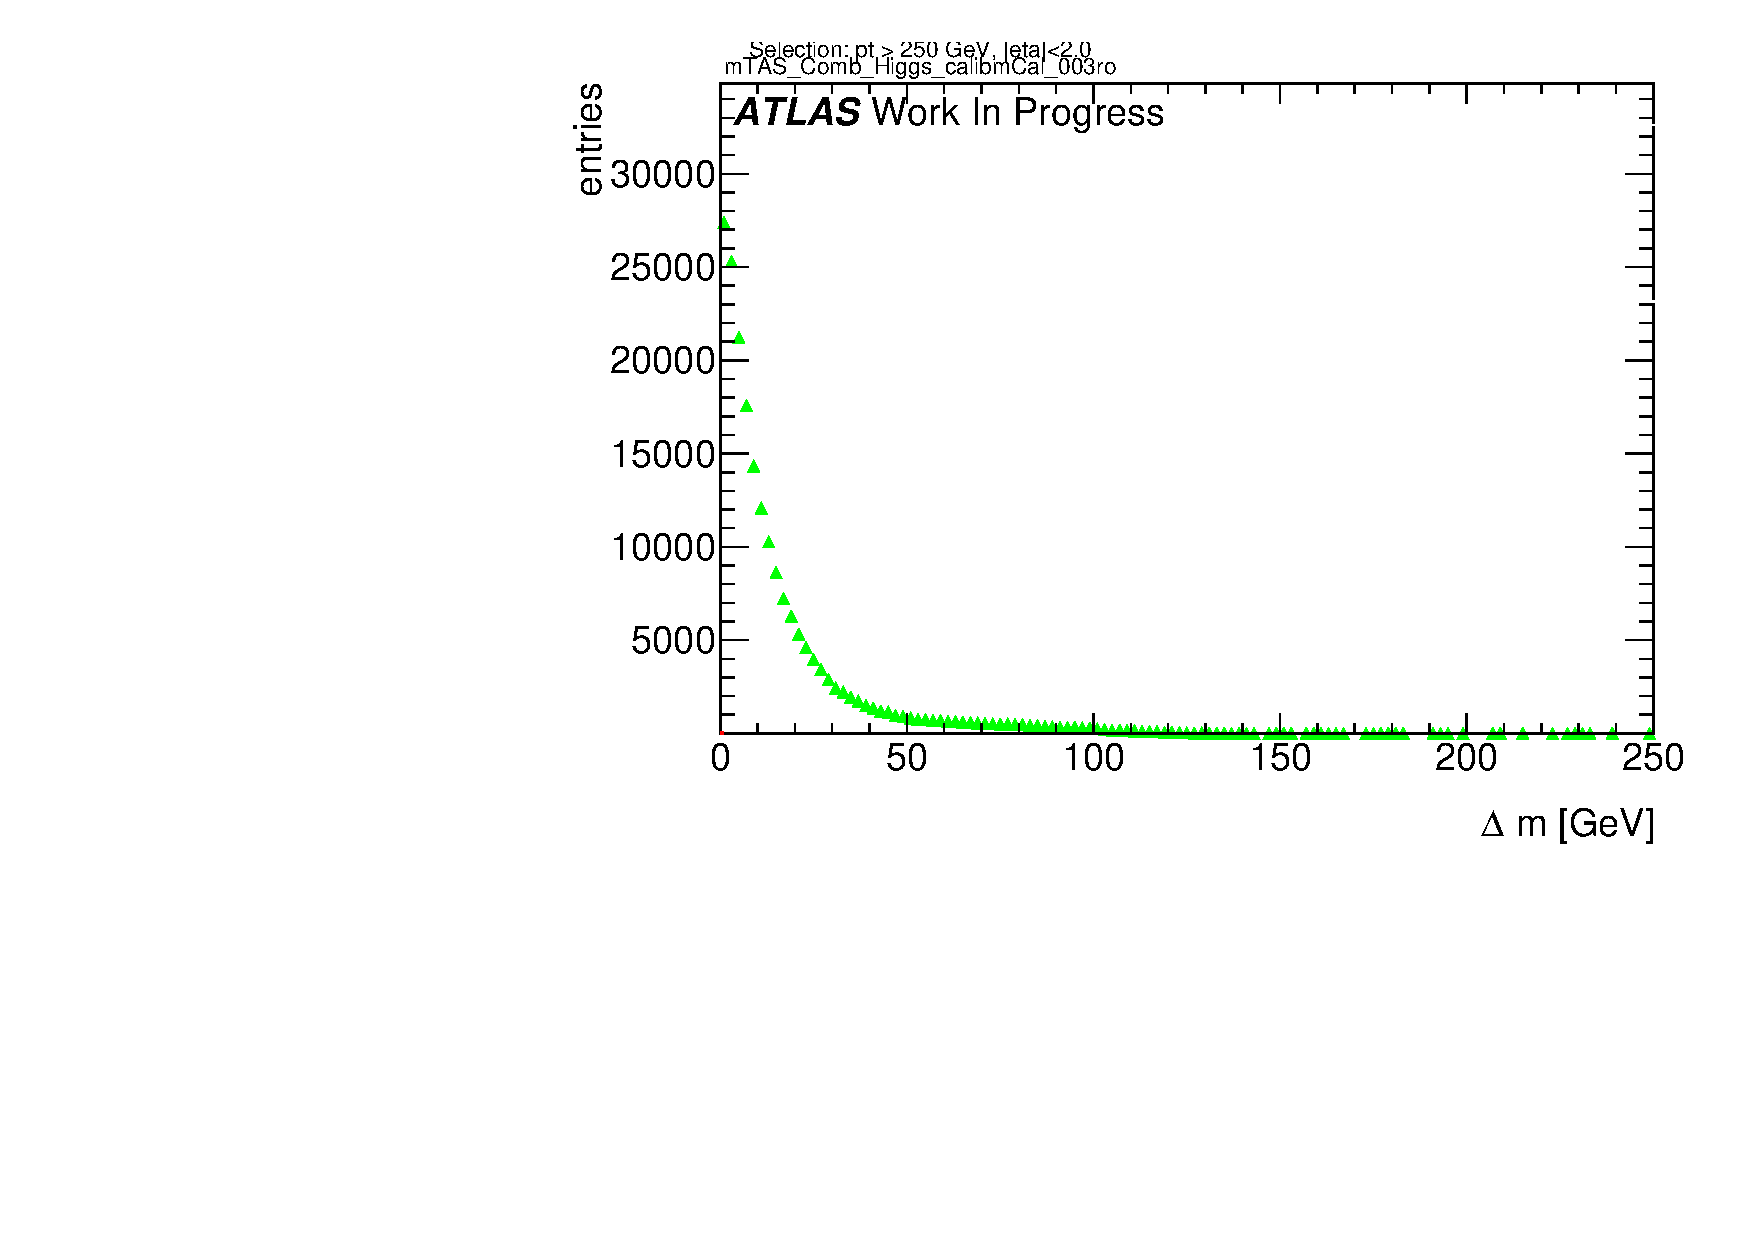
\includegraphics[width=0.4\textwidth]{/Users/fabnap/Documents/MasterArbeit/appendixB/mTAS_W_calibmCal_20:07:01-03-11-2016/1cfrt_h_SubJet_Delta_m.pdf}
\caption{$| m_{sub-jet} - m_{track-jet} |$ distribution, where sub-jet and track-jet are the closest}
 
\end{figure}
 
\begin{figure}
 
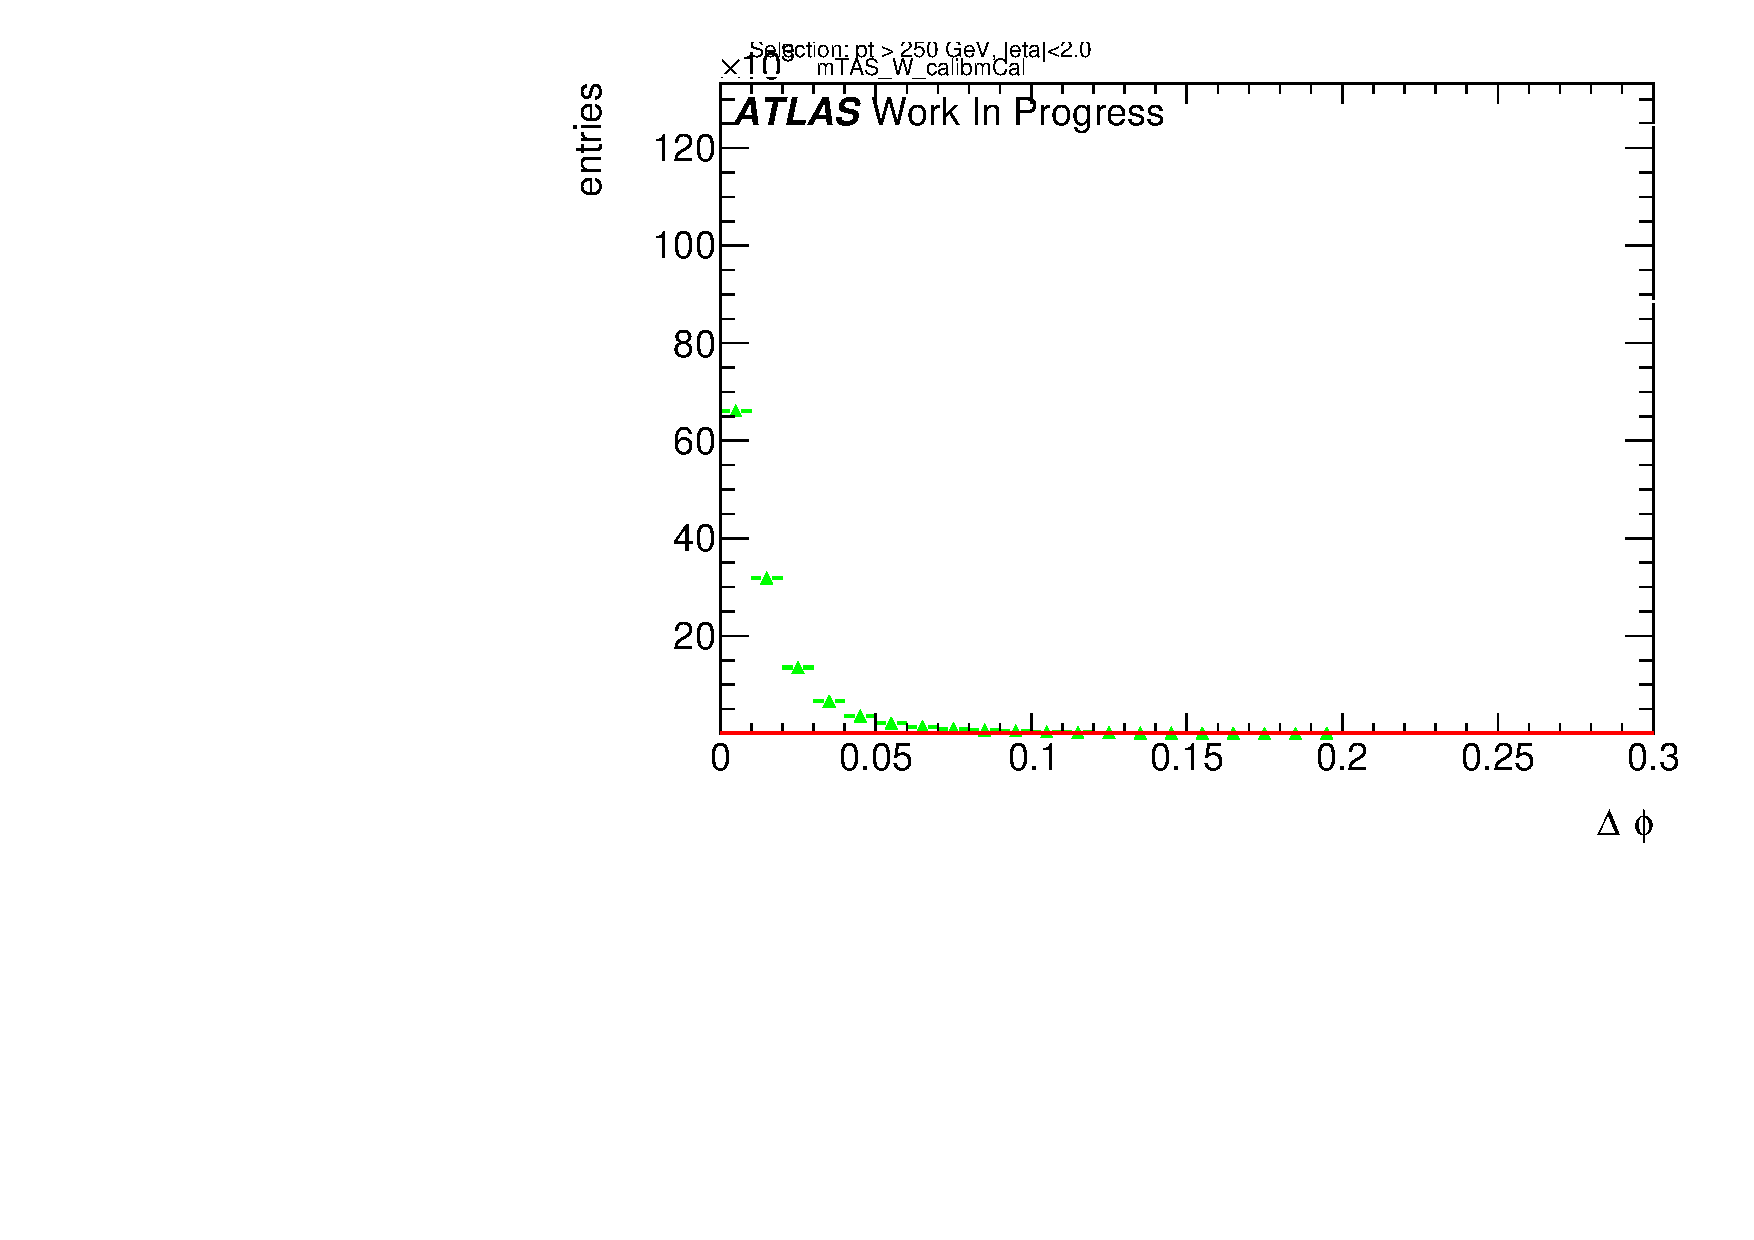
\includegraphics[width=0.4\textwidth]{/Users/fabnap/Documents/MasterArbeit/appendixB/mTAS_W_calibmCal_20:07:01-03-11-2016/1cfrt_h_SubJet_Delta_psi.pdf}
\caption{$| \phi_{sub-jet} - \phi_{track-jet} | $ distribution, where sub-jet and track-jet are the closest}
 
\end{figure}
 %
\begin{figure}
 
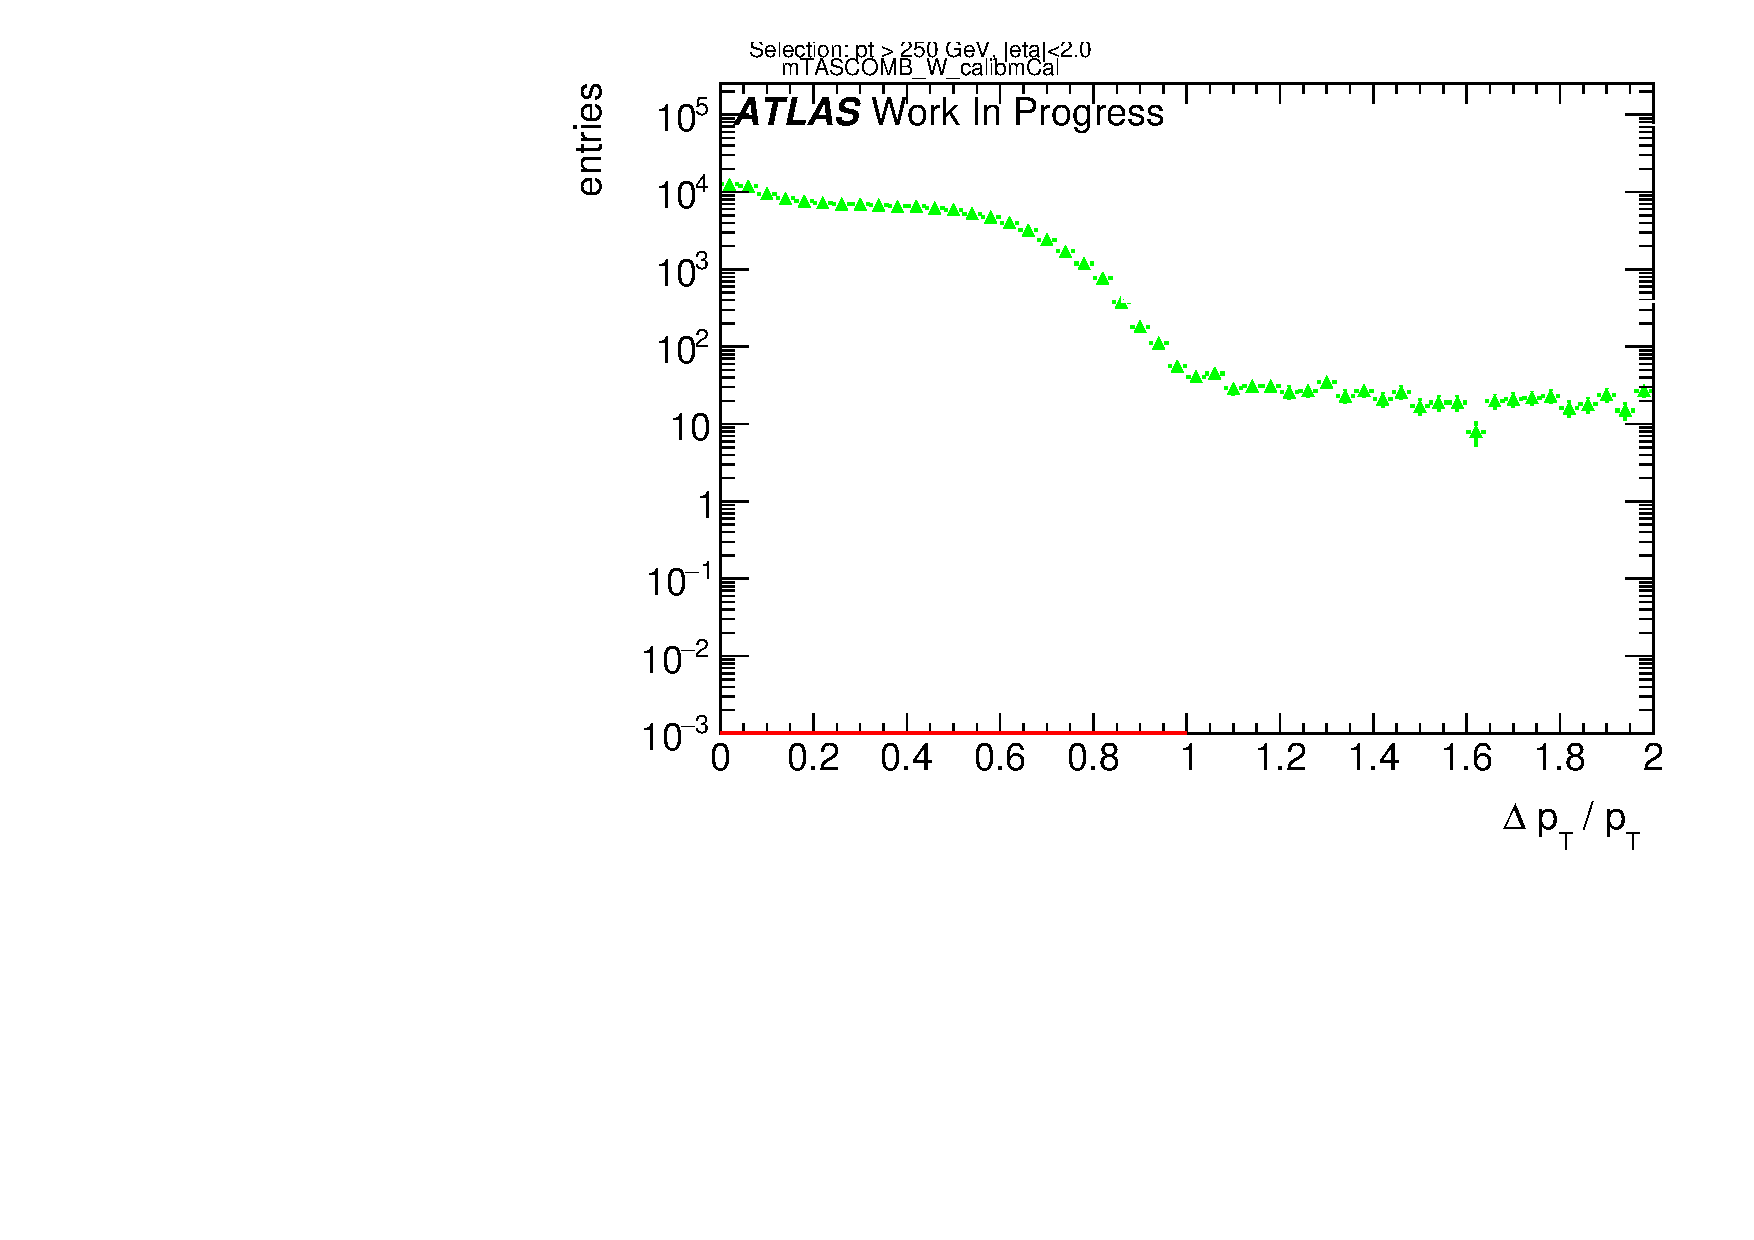
\includegraphics[width=0.4\textwidth]{/Users/fabnap/Documents/MasterArbeit/appendixB/mTAS_W_calibmCal_20:07:01-03-11-2016/1cfrt_h_SubJet_Delta_pt.pdf}
\caption{$| p_{T,sub-jet} - p_{T,track-jet} | $ distribution, where sub-jet and track-jet are the closest}
 
\end{figure}
 
\begin{figure}
 
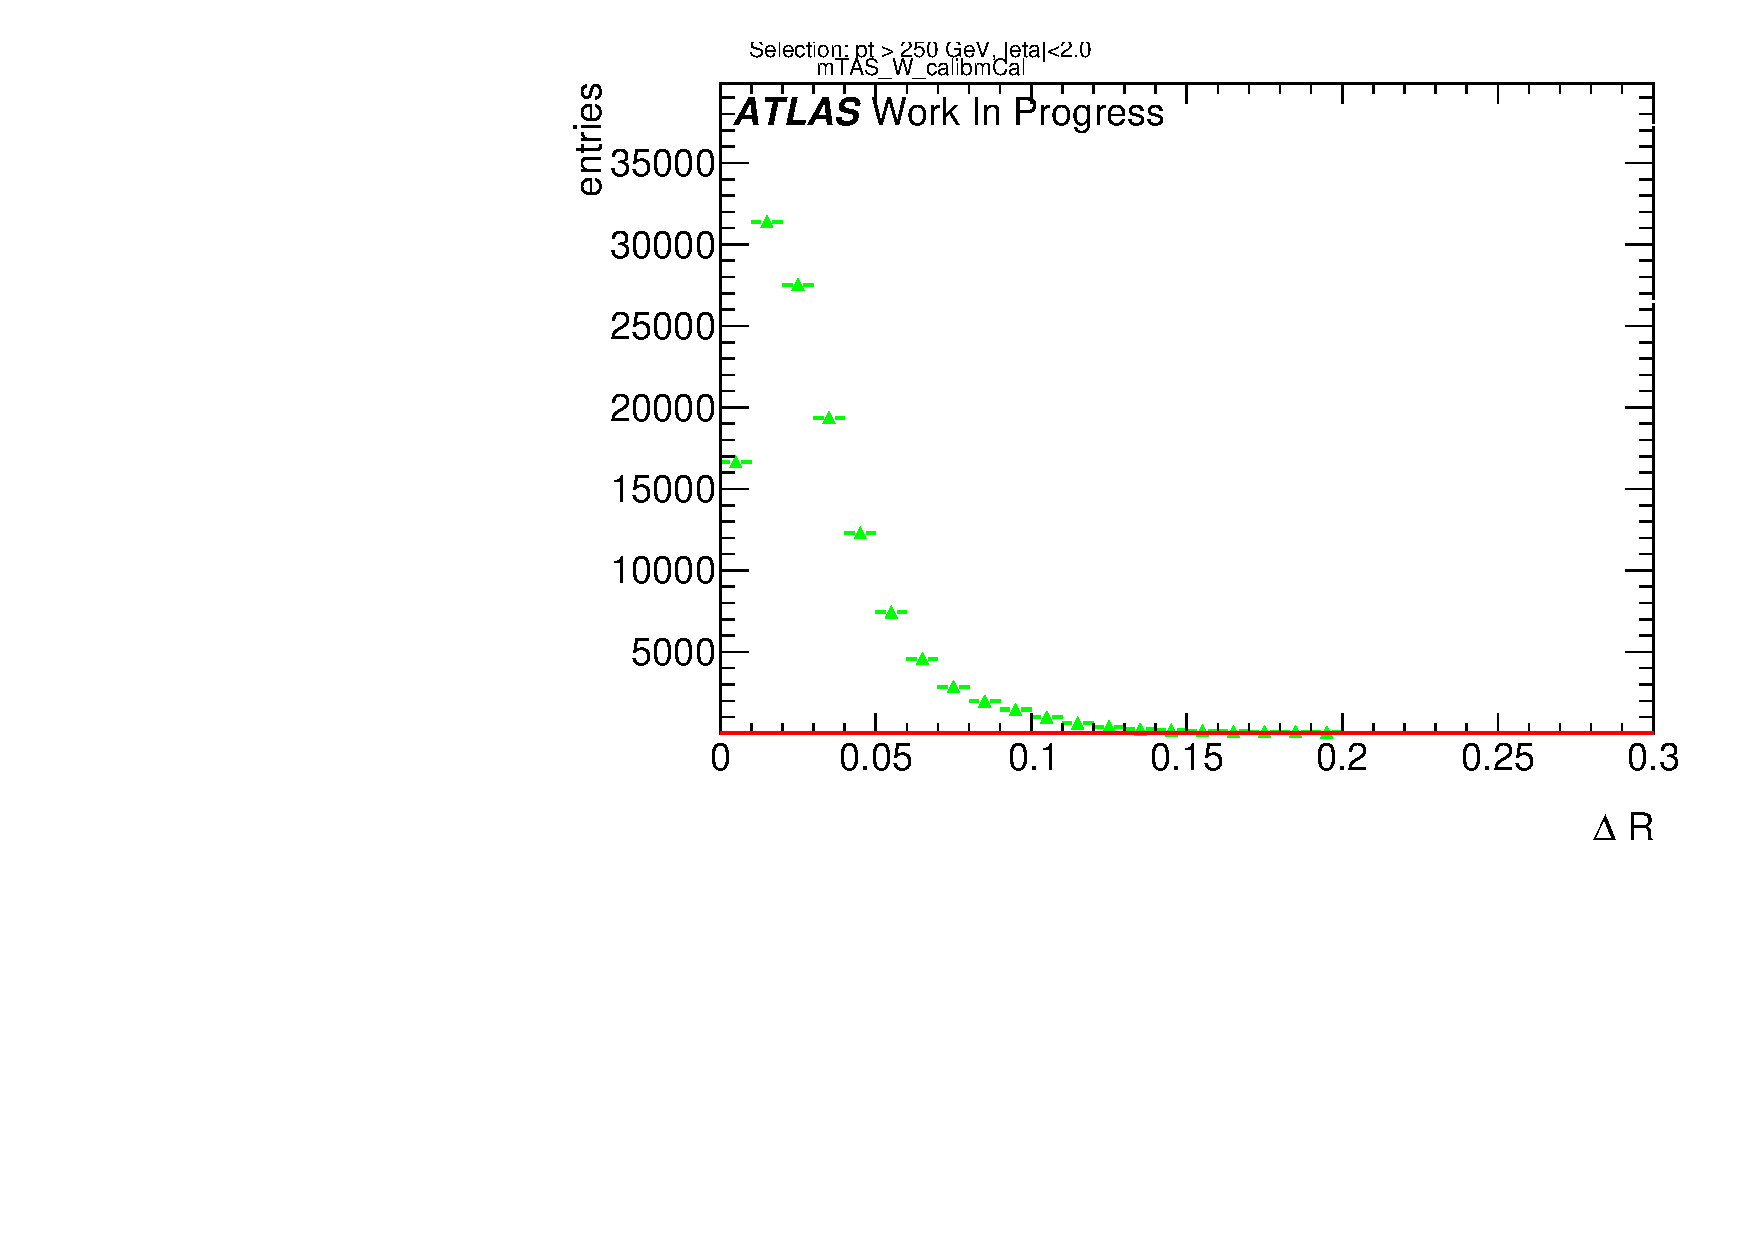
\includegraphics[width=0.4\textwidth]{/Users/fabnap/Documents/MasterArbeit/appendixB/mTAS_W_calibmCal_20:07:01-03-11-2016/1cfrt_h_SubJet_Delta_R.pdf}
\caption{$| R_{sub-jet} - R_{track-jet} | $ distribution, where sub-jet and track-jet are the closest}
 
\end{figure}
 
\begin{figure}
 
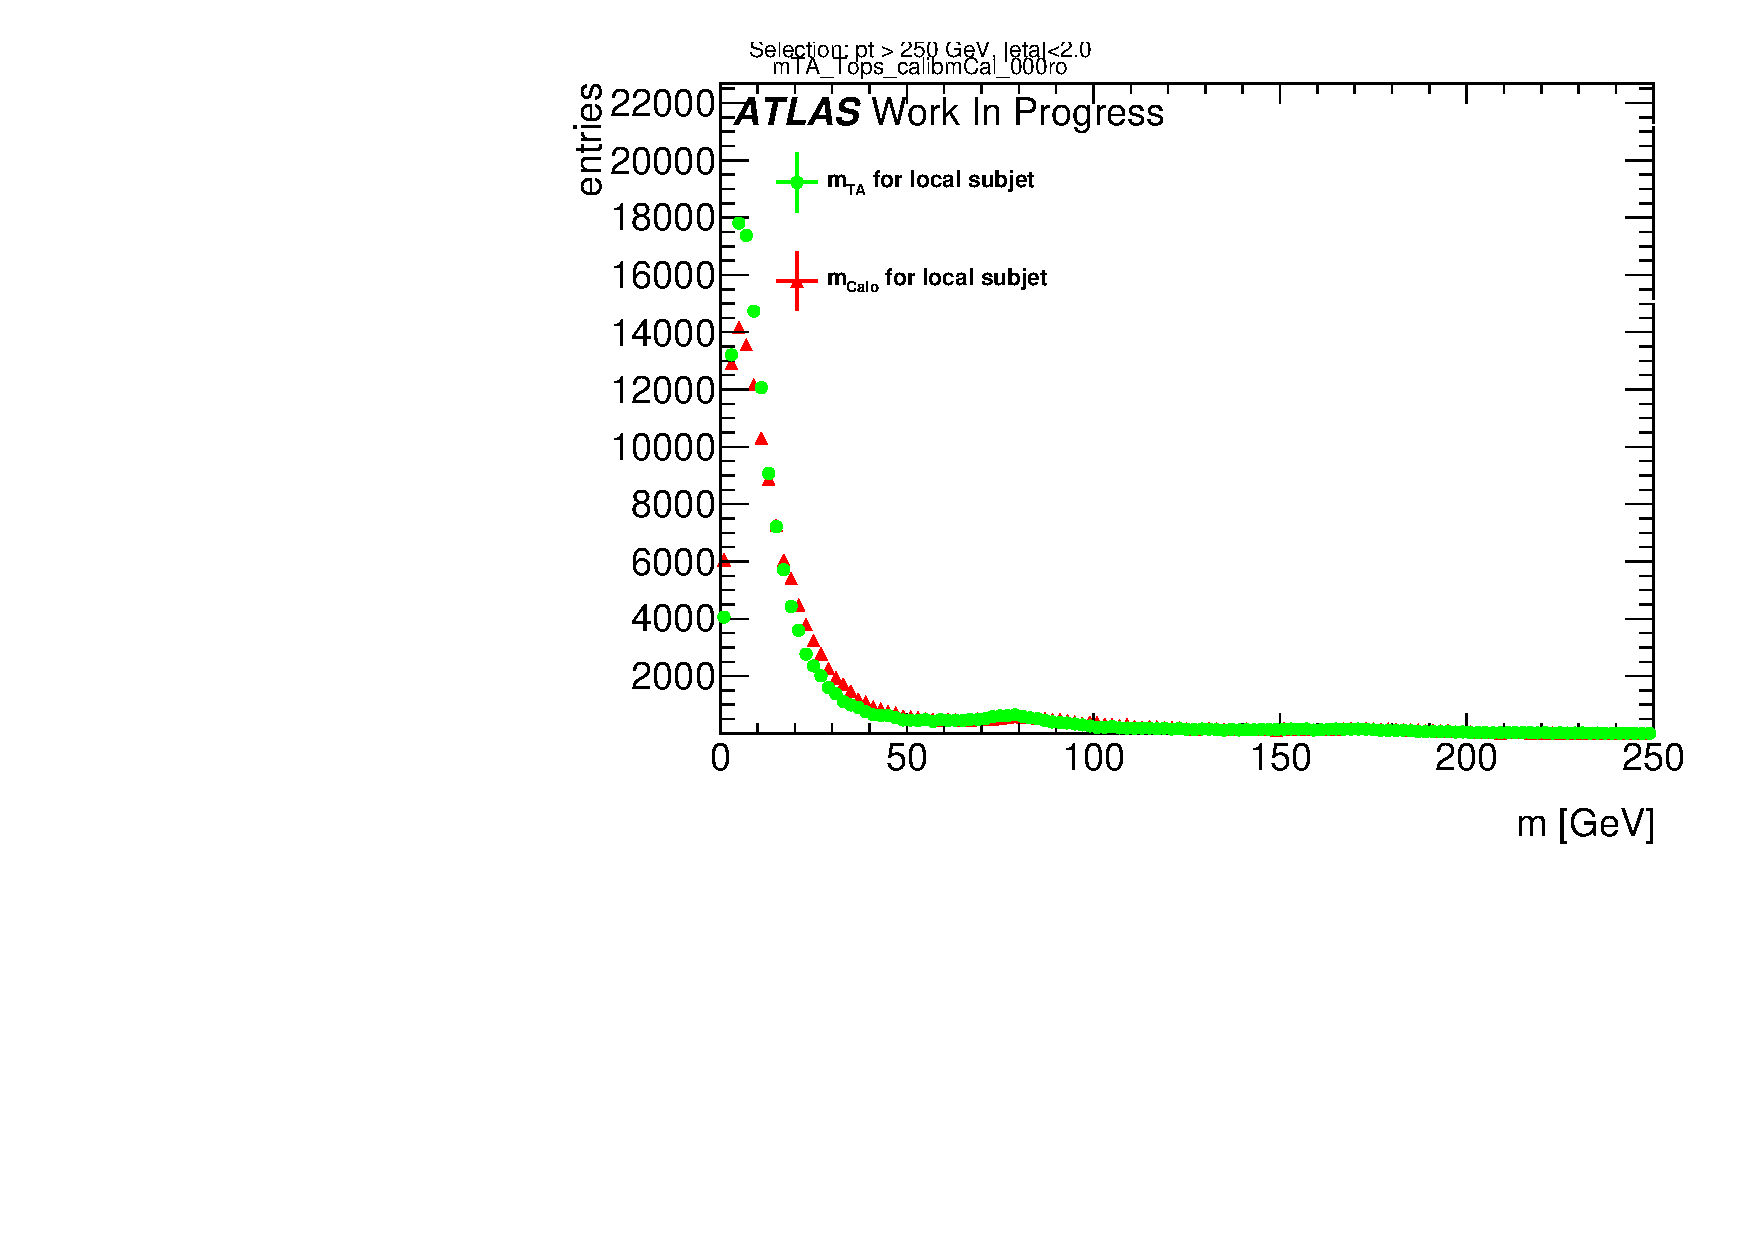
\includegraphics[width=0.4\textwidth]{/Users/fabnap/Documents/MasterArbeit/appendixB/mTAS_W_calibmCal_20:07:01-03-11-2016/1cfrt_h_SubJet_m.pdf}
\caption{Mass distribution of the sub-jet, calorimeter and track-assisted}
 
\end{figure}
 
\begin{figure}
 
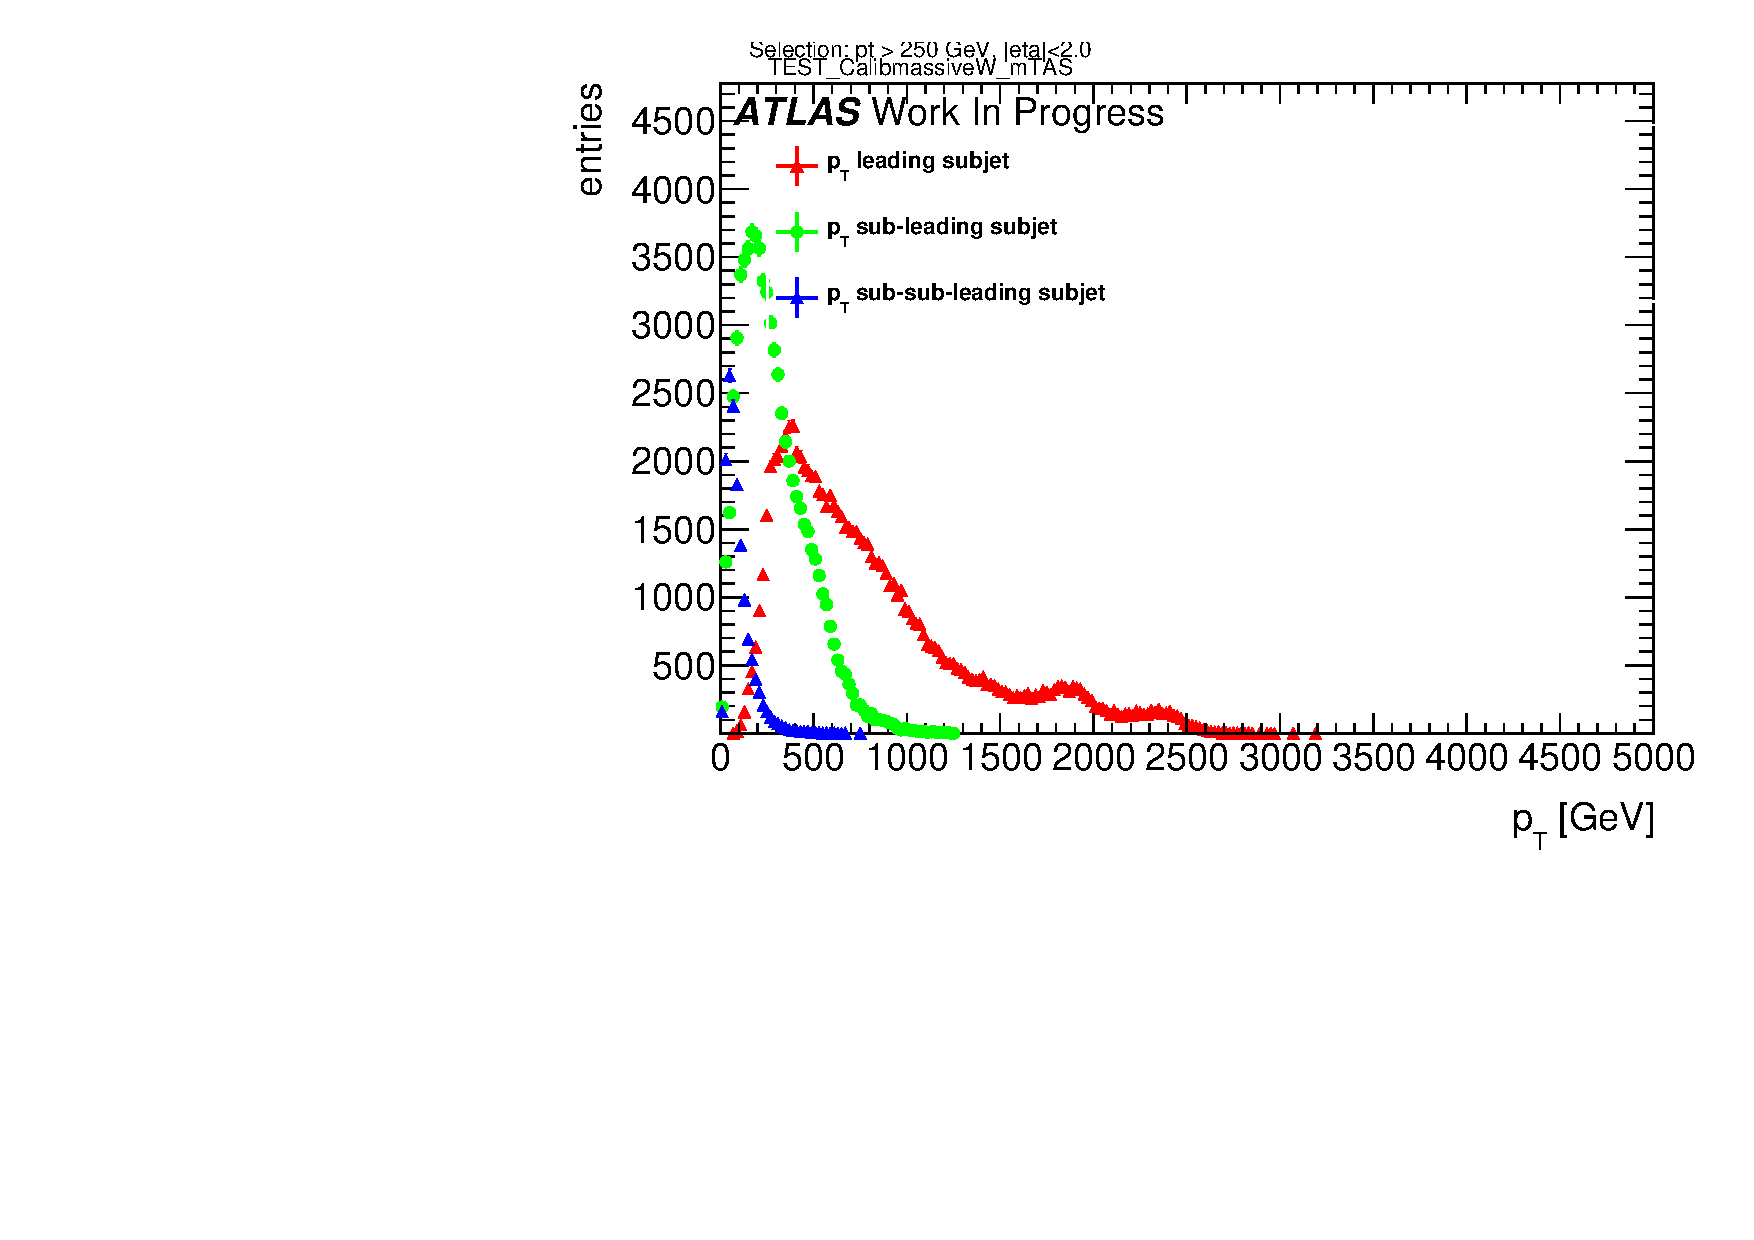
\includegraphics[width=0.4\textwidth]{/Users/fabnap/Documents/MasterArbeit/appendixB/mTAS_W_calibmCal_20:07:01-03-11-2016/1cfrt_h_SubJet_pt1.pdf}
\caption{$\pt$ distribution for leading, sub-leading and sub-sub-leading sub-jets}
 
\end{figure}
 %
\begin{figure}
 
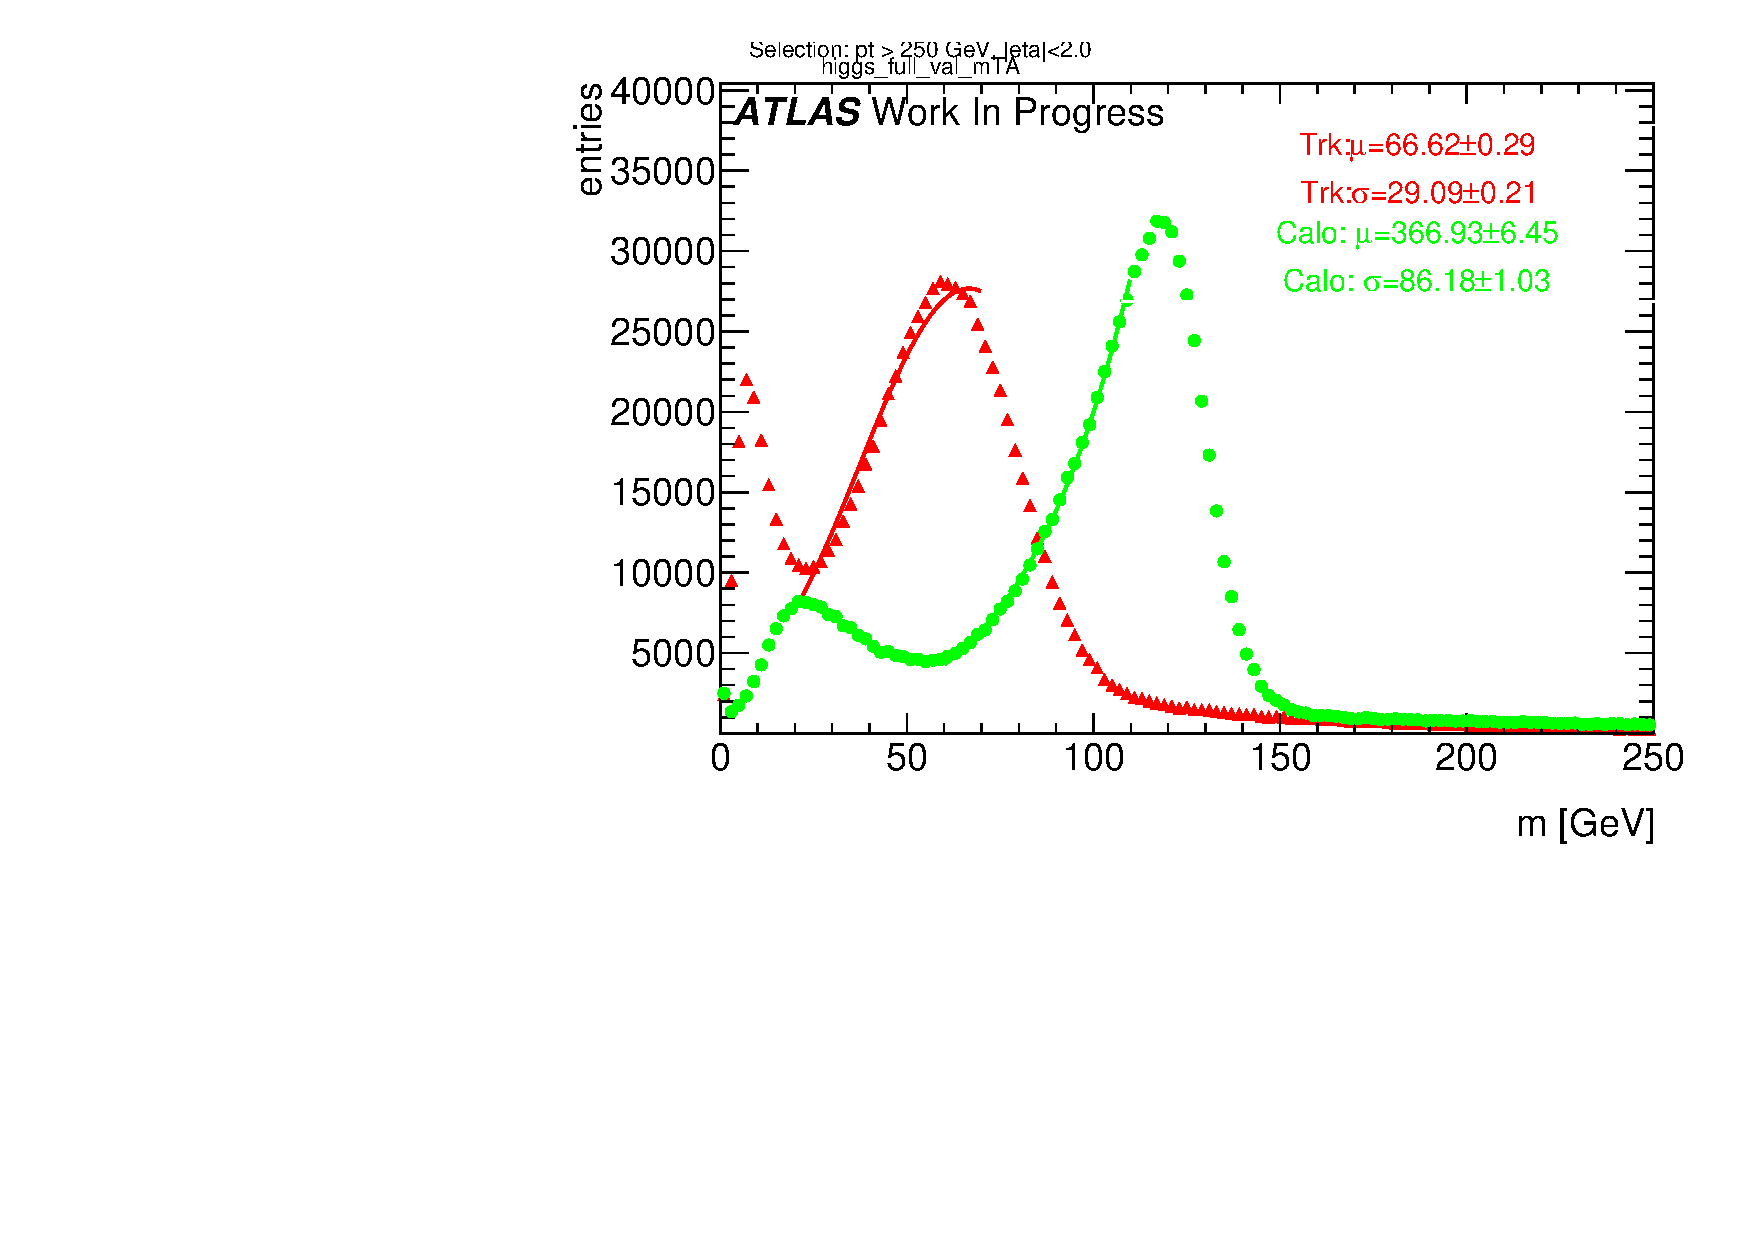
\includegraphics[width=0.4\textwidth]{/Users/fabnap/Documents/MasterArbeit/appendixB/mTAS_W_calibmCal_20:07:01-03-11-2016/1cfrt_h_TrackJets_m.pdf}
\caption{Mass distribution for calorimeter and tracks associated to the large-R jet}
 
\end{figure}
 
\begin{figure}
 
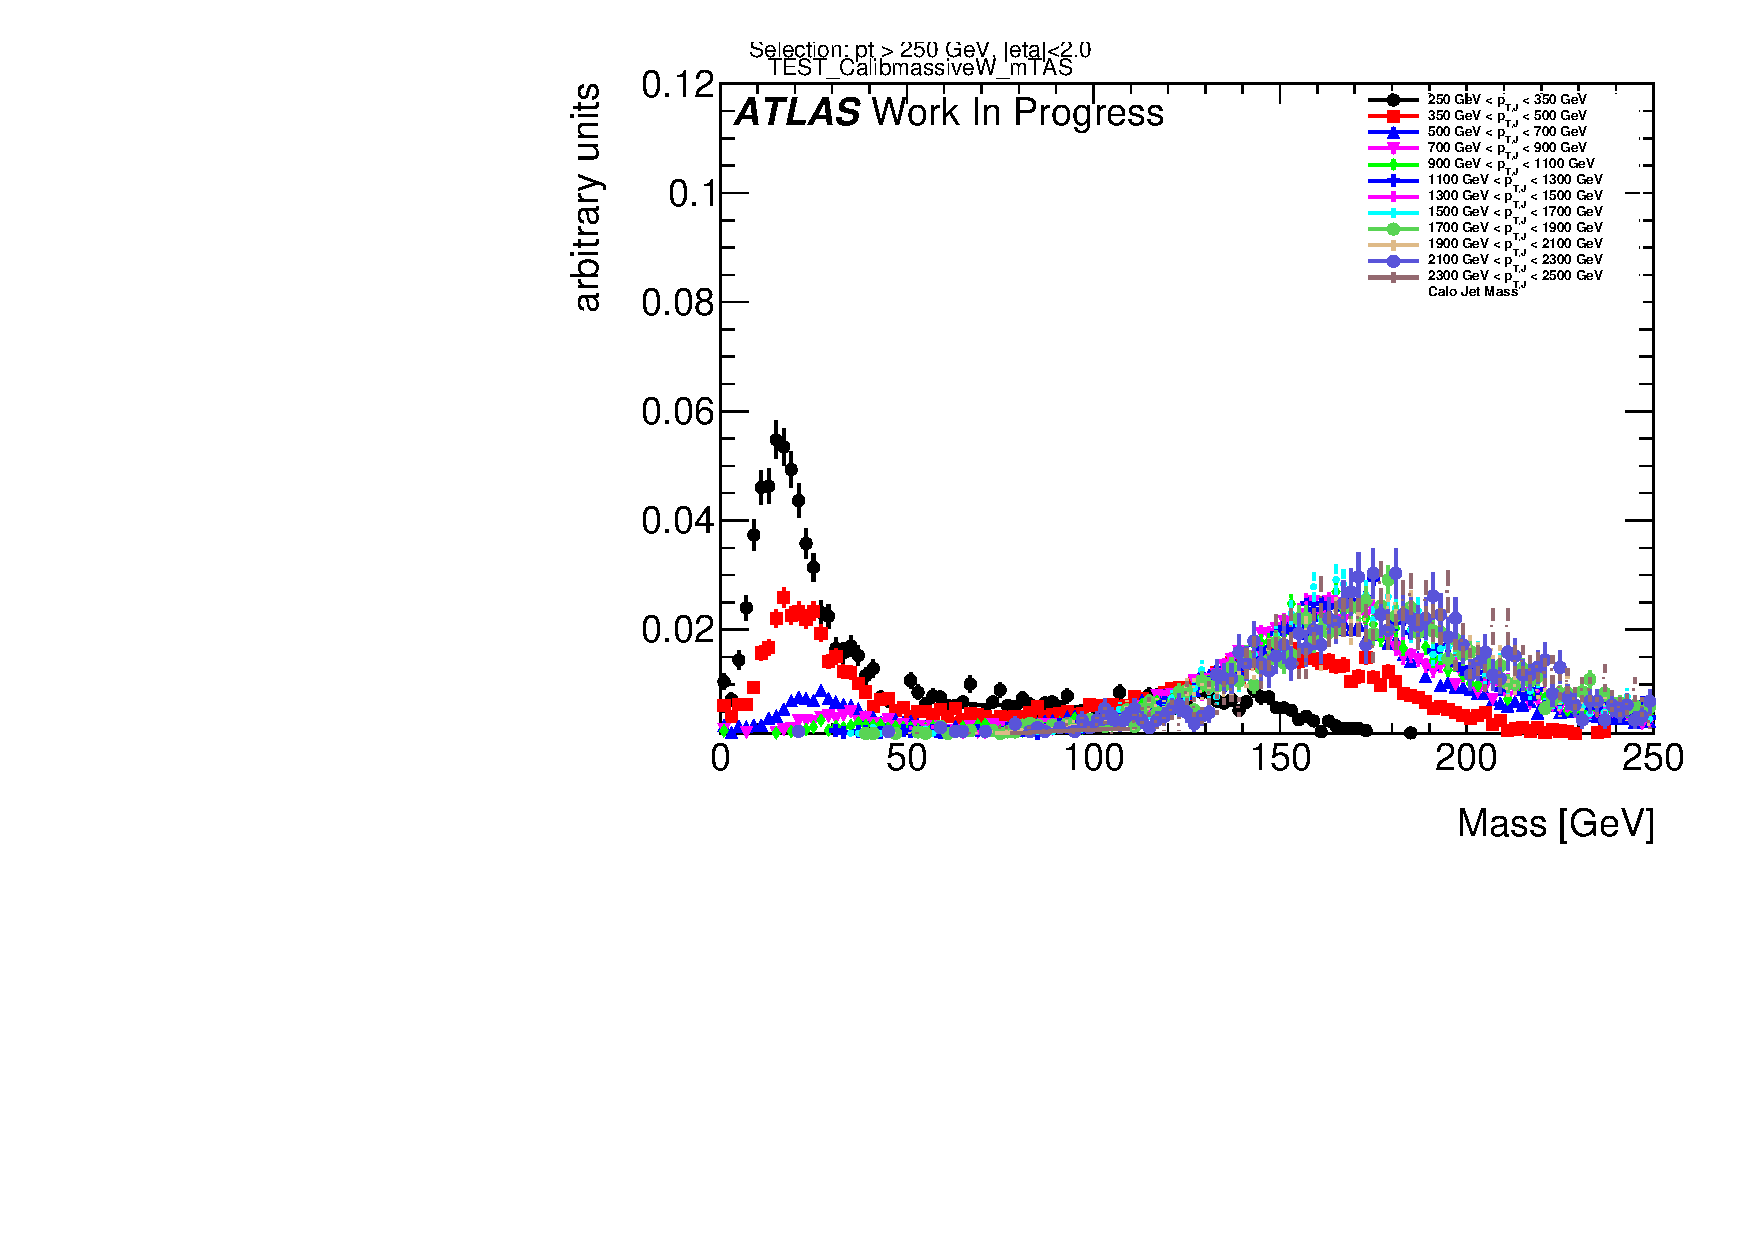
\includegraphics[width=0.4\textwidth]{/Users/fabnap/Documents/MasterArbeit/appendixB/mTAS_W_calibmCal_20:07:01-03-11-2016/2cfrt_h_FatJet_ptJ12m_mervM.pdf}
\caption{$\mcal$ for $p_{T}^{J}$ bin, superimposed}
 
\end{figure}
 
\begin{figure}

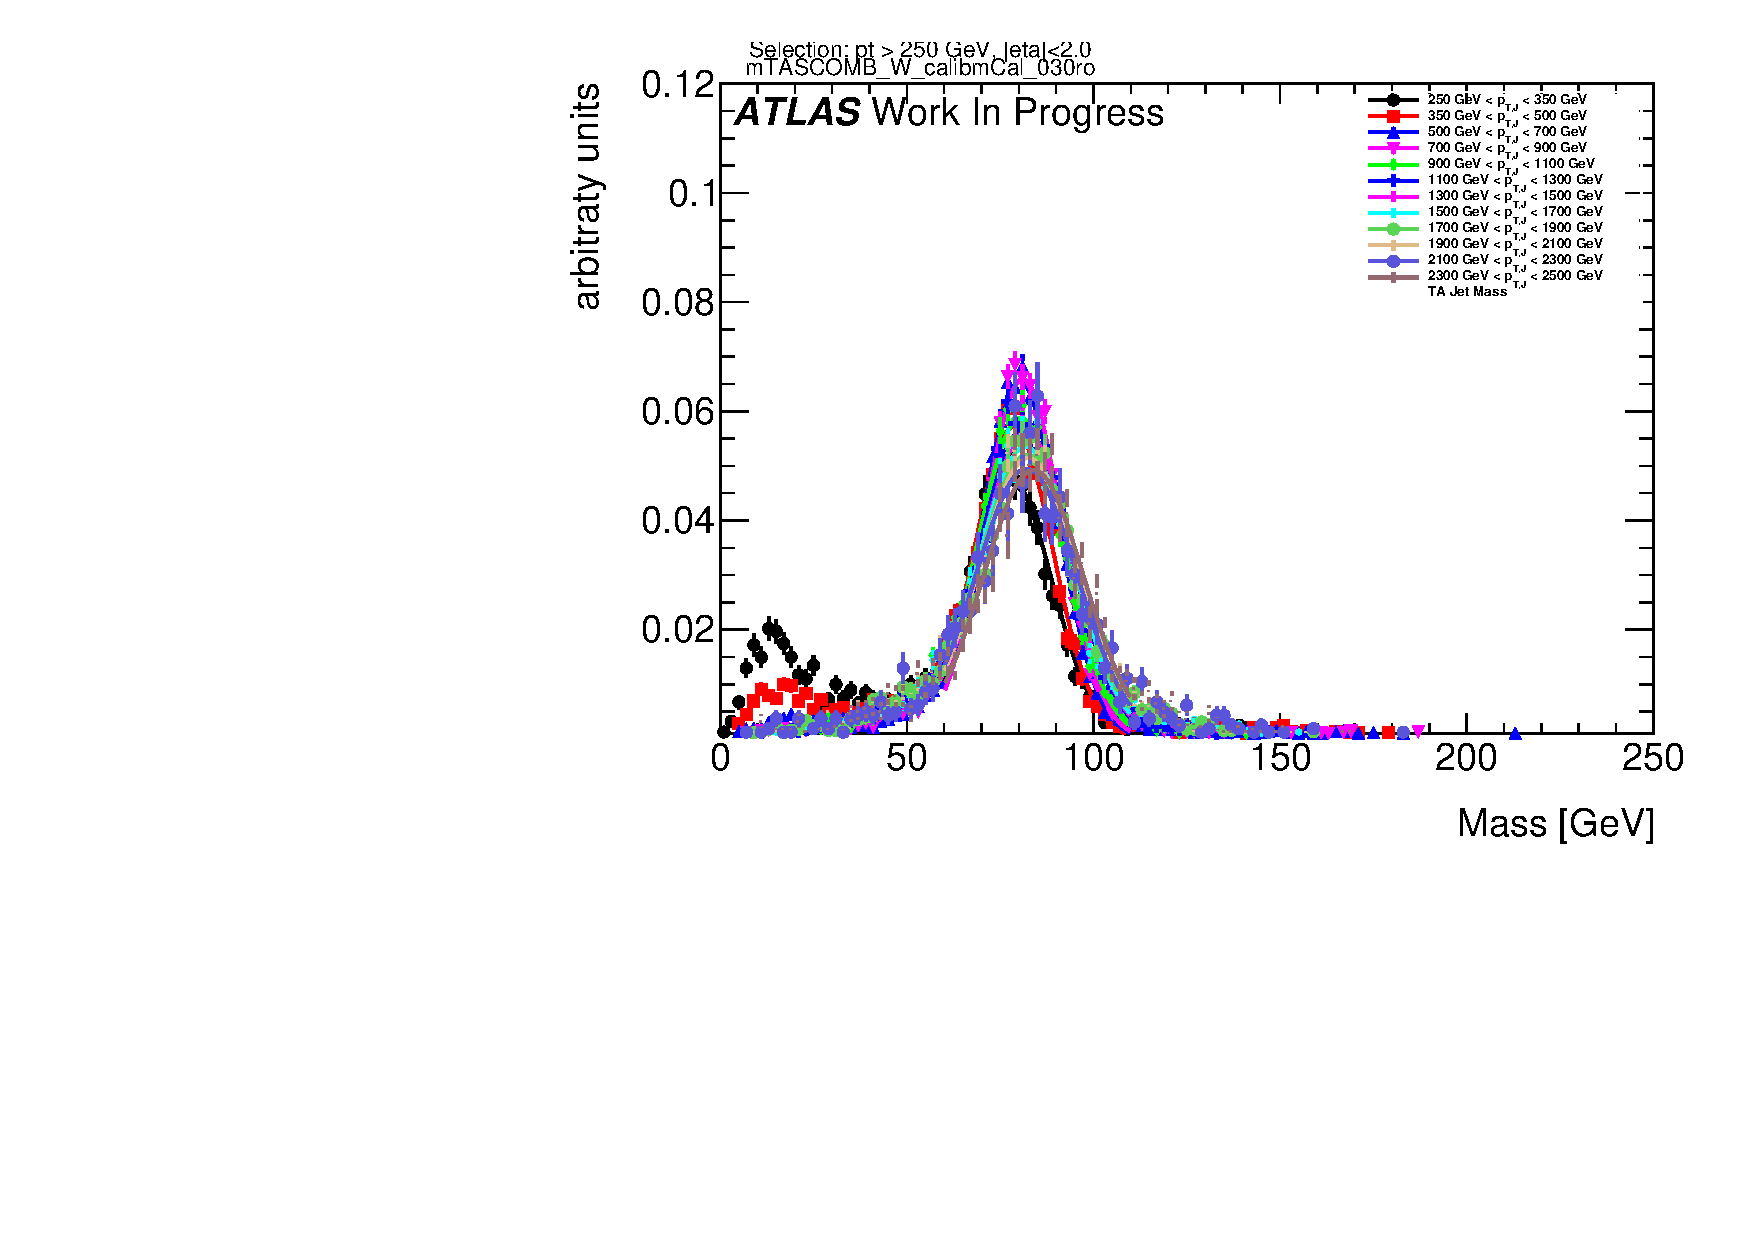
\includegraphics[width=0.4\textwidth]{/Users/fabnap/Documents/MasterArbeit/appendixB/mTAS_W_calibmCal_20:07:01-03-11-2016/3cfrt_h_FatJet_ptJ12TAm_mervTA.pdf}
\caption{$\mtas$ for $p_{T}^{J}$ bin, superimposed}

\end{figure}

\begin{figure}

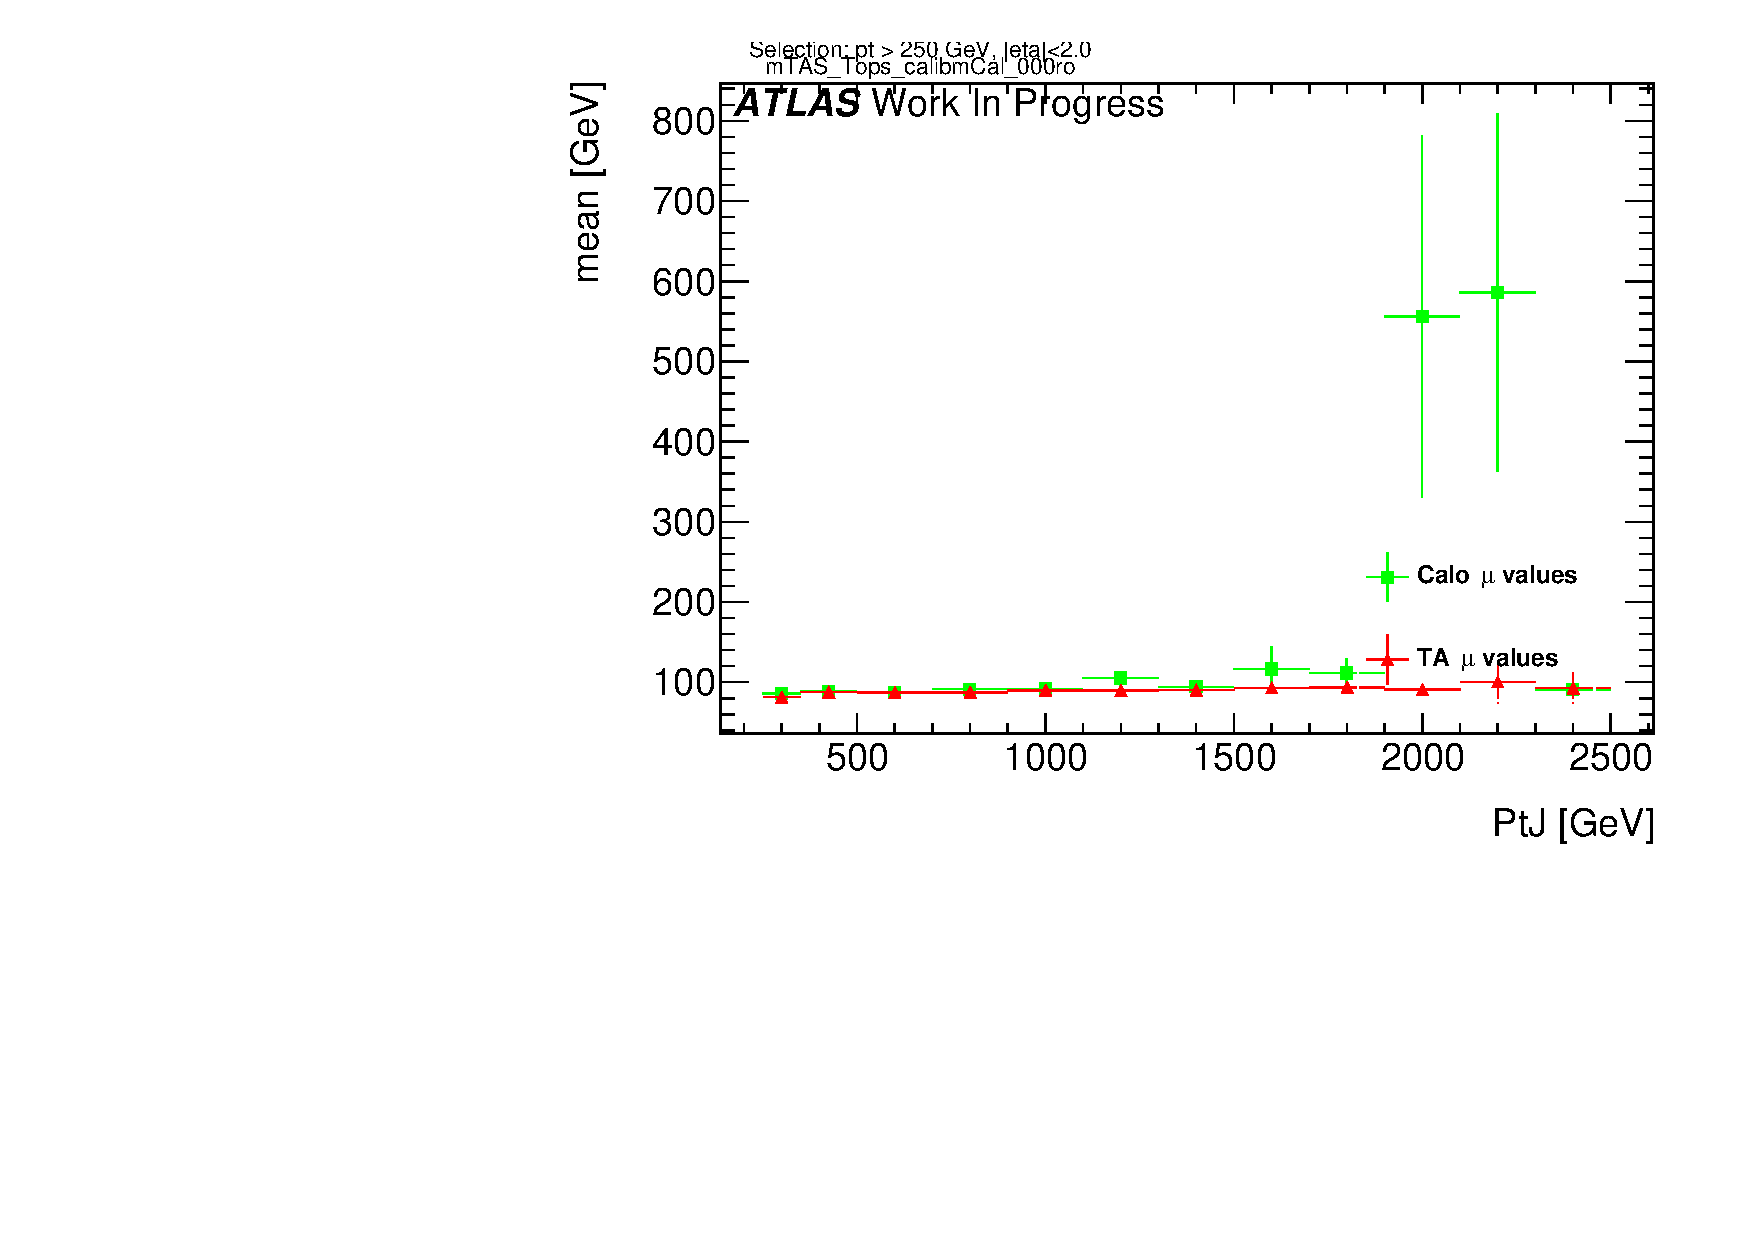
\includegraphics[width=0.4\textwidth]{/Users/fabnap/Documents/MasterArbeit/appendixB/mTAS_W_calibmCal_20:07:01-03-11-2016/5graph_h_FatJet_ptJ12m_meanMvsTA.pdf}
\caption{$\mu$ from fit of the mass distribution vs bin of $p_{T}^{J}$ }

\end{figure}

\begin{figure}

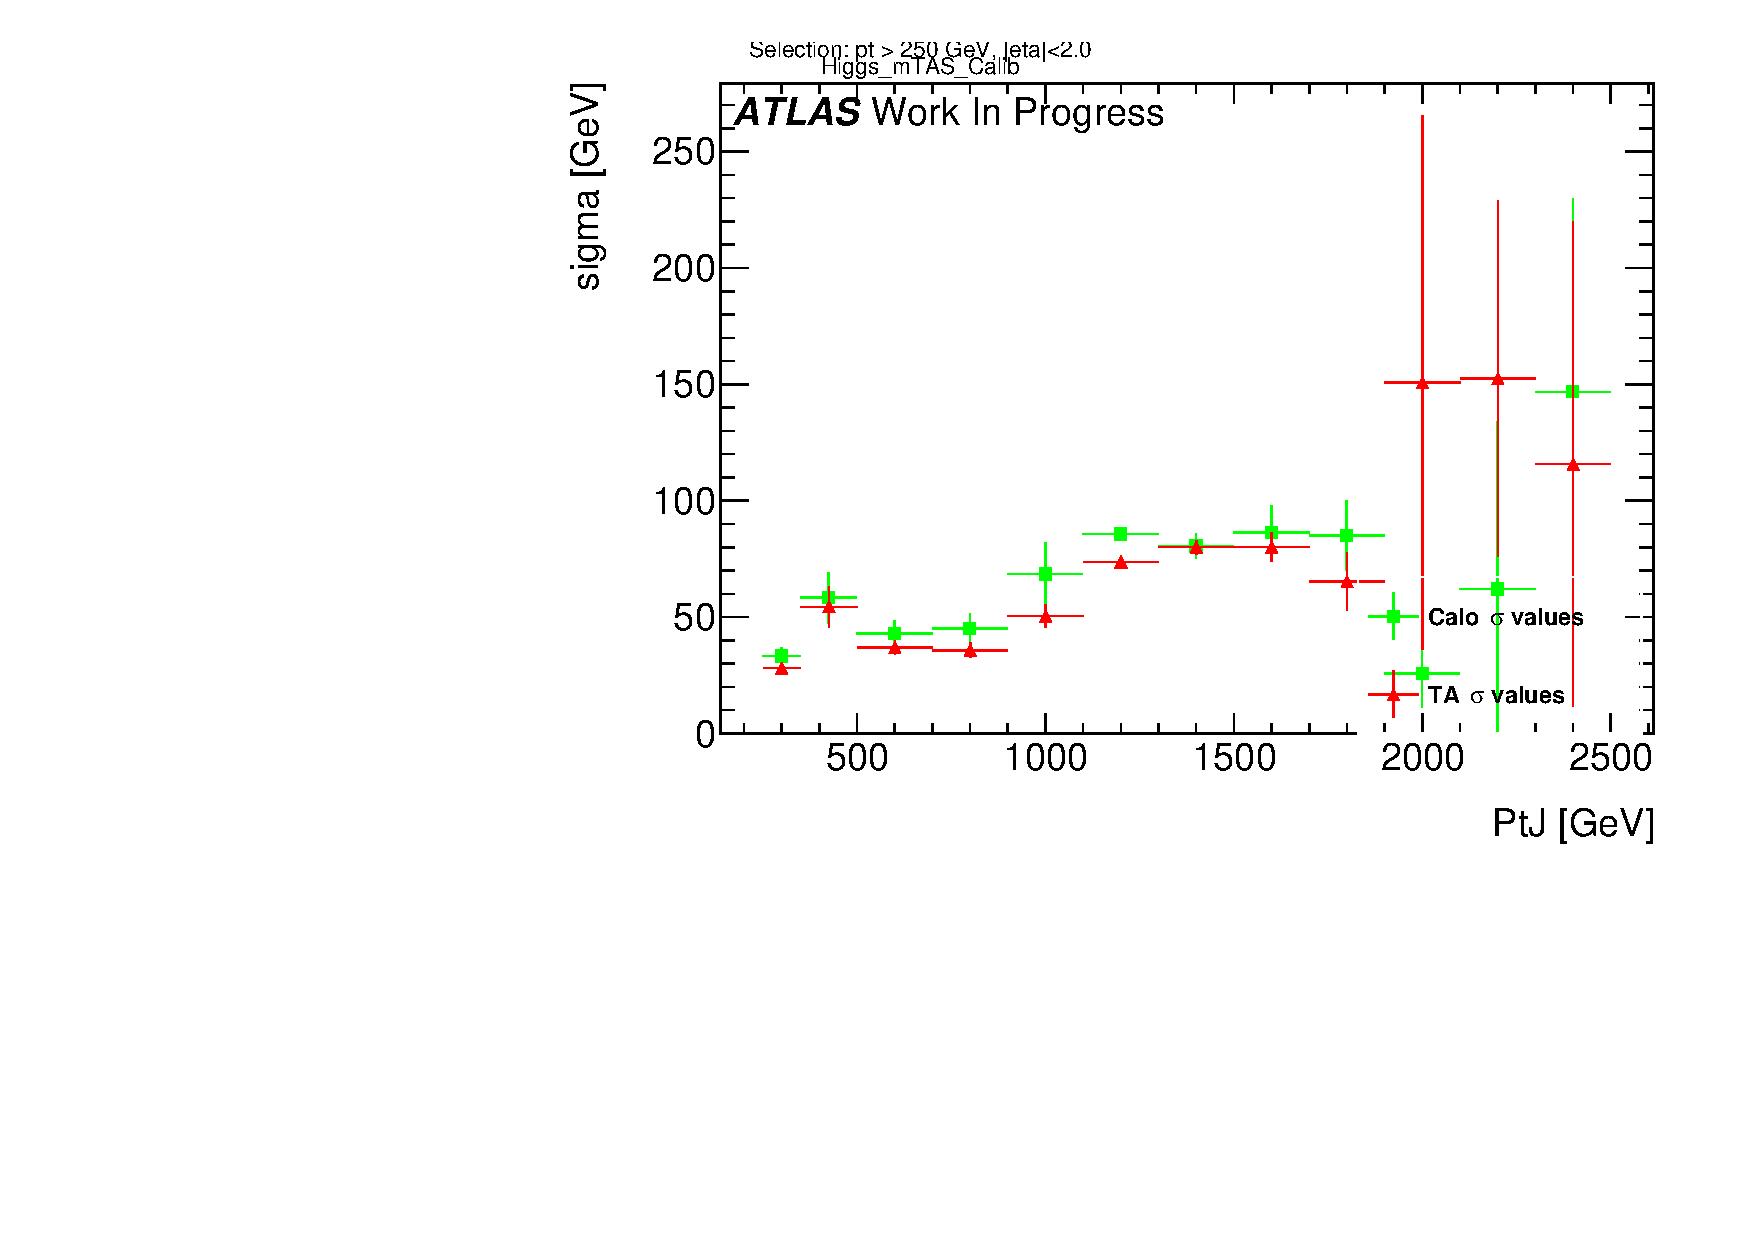
\includegraphics[width=0.4\textwidth]{/Users/fabnap/Documents/MasterArbeit/appendixB/mTAS_W_calibmCal_20:07:01-03-11-2016/6graph_h_FatJet_ptJ12m_sigmaMvsTA.pdf}
\caption{$\sigma$ from fit of the mass distribution vs bin of $p_{T}^{J}$ }

\end{figure}

\clearpage

\begin{figure}

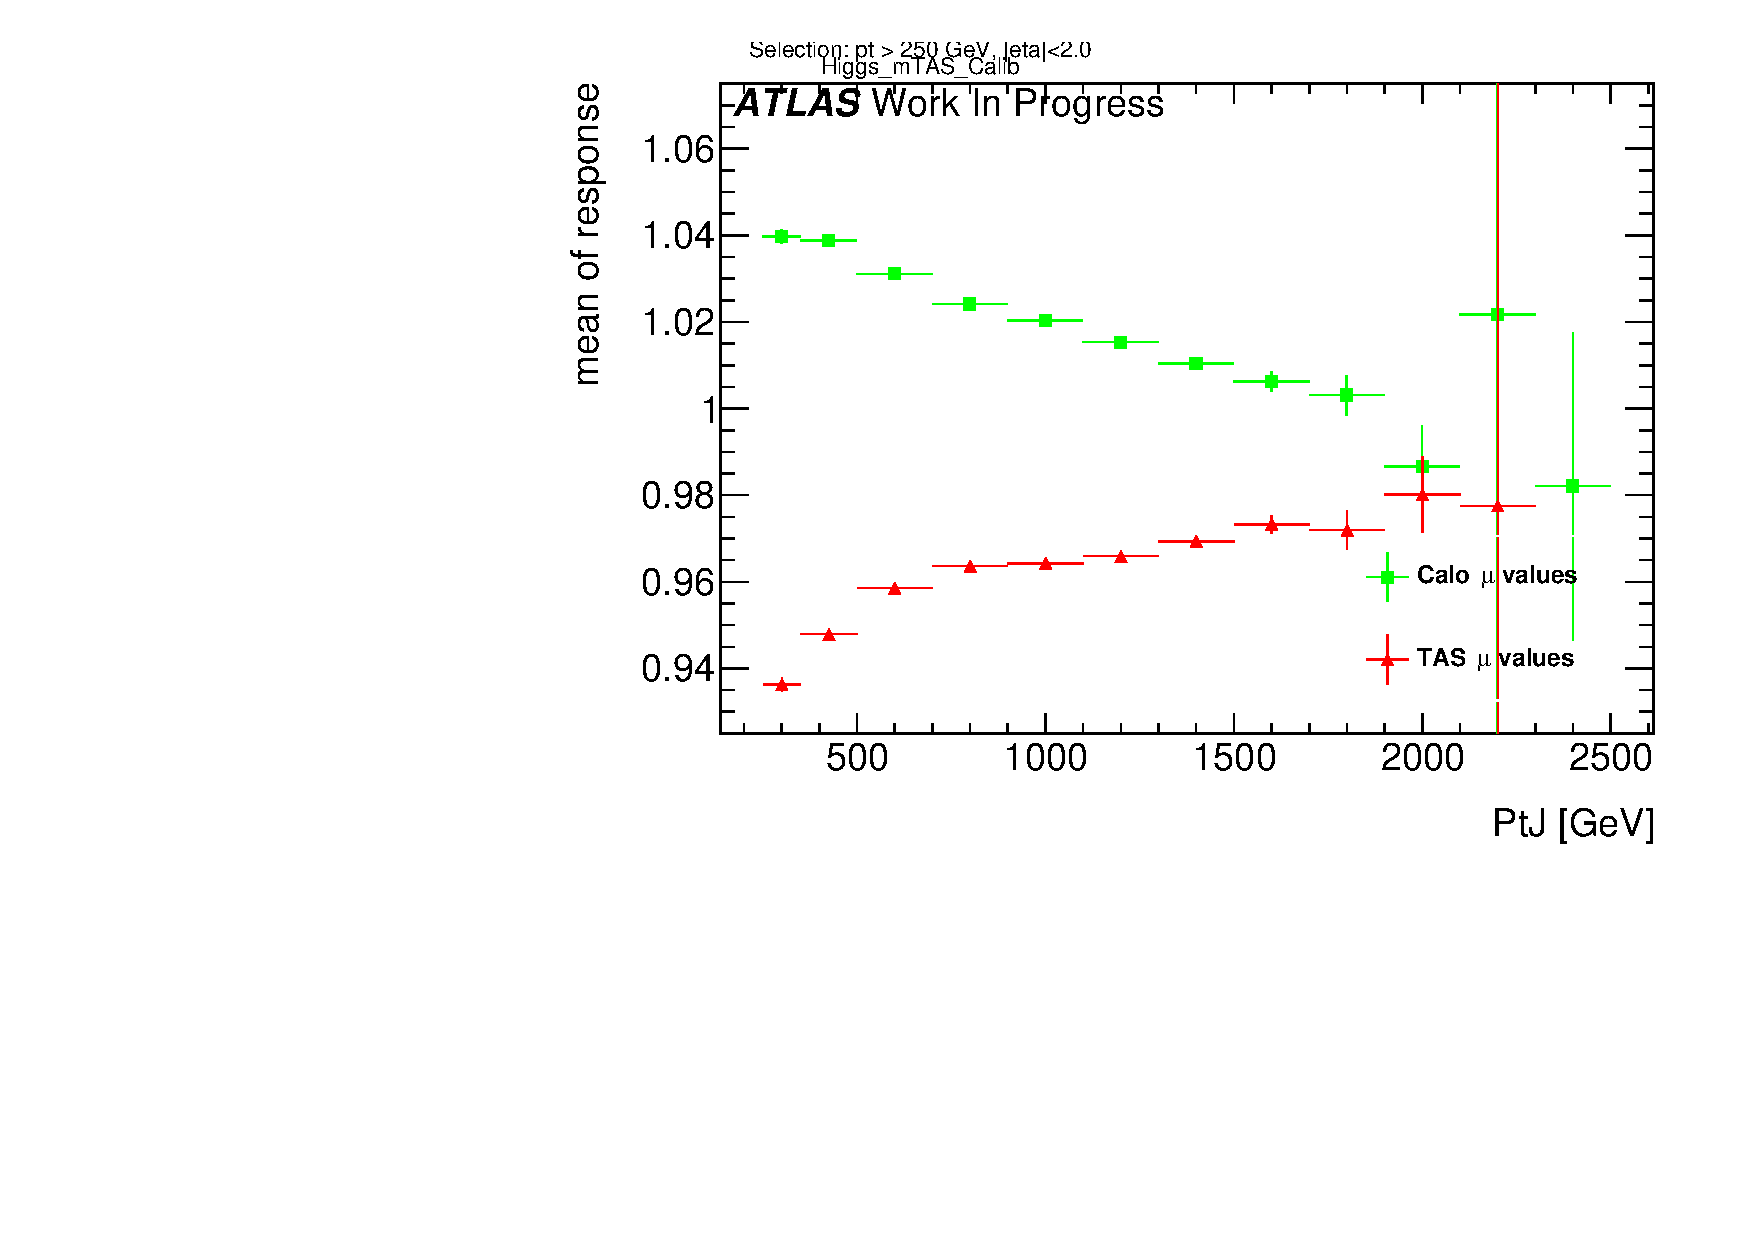
\includegraphics[width=0.4\textwidth]{/Users/fabnap/Documents/MasterArbeit/appendixB/mTAS_W_calibmCal_20:07:01-03-11-2016/71graph_h_JetRatio_mJ12CALO_meanResponseMvsTA.pdf}
\caption{$\mu $ from fit of the mass Response vs bin of  $p_{T}^{J}$}

\end{figure}
 %
\begin{figure}

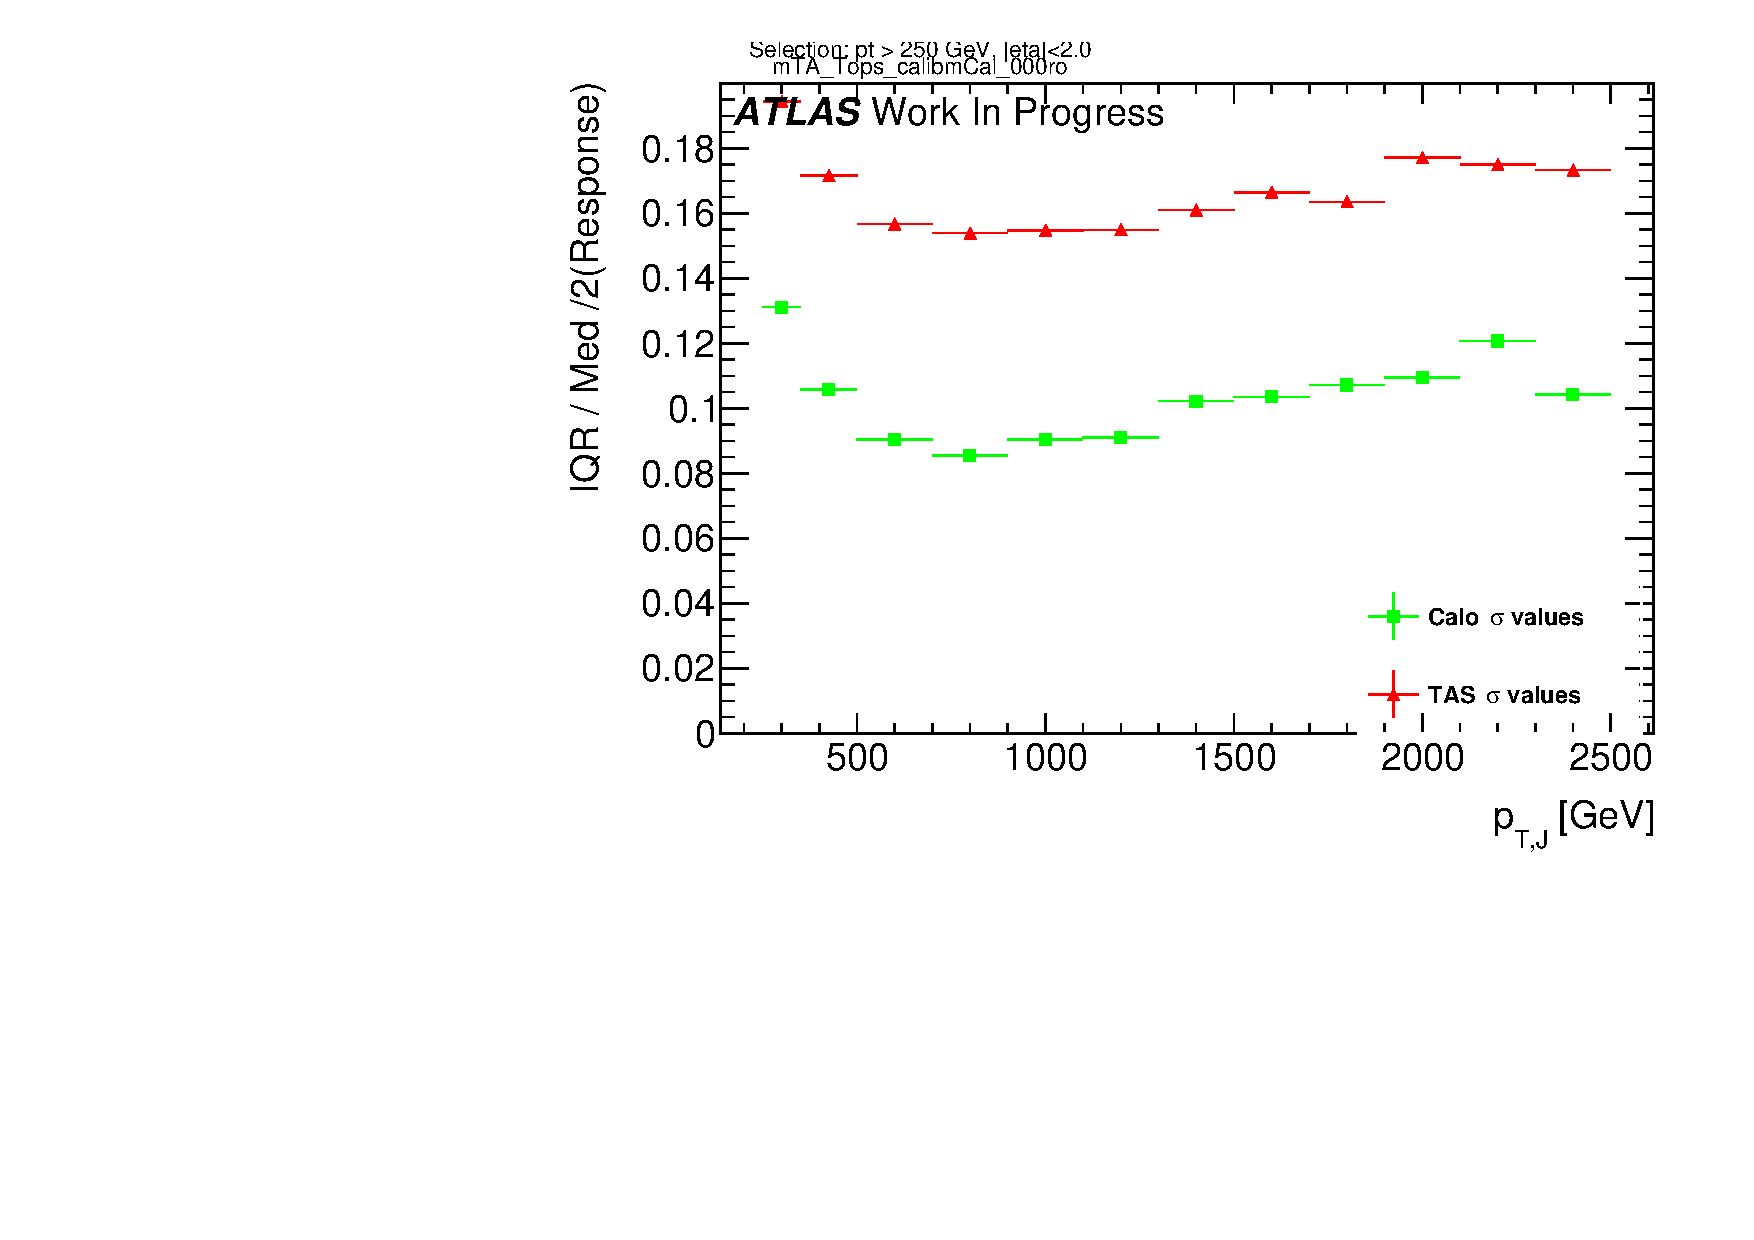
\includegraphics[width=0.4\textwidth]{/Users/fabnap/Documents/MasterArbeit/appendixB/mTAS_W_calibmCal_20:07:01-03-11-2016/72graph_h_JetRatio_mJ12CALO_sigmaResponseMvsTA.pdf}
\caption{$\sigma $ from fit of the mass Response vs bin of $p_{T}^{J}$}

\end{figure}

\begin{figure}

\includegraphics[width=0.4\textwidth]{/Users/fabnap/Documents/MasterArbeit/appendixB/mTAS_W_calibmCal_20:07:01-03-11-2016/73graph_h_JetRatio_mJ12CALO_I50ResponseMvsTA.pdf}
\caption{Left integral, $\int_{0}^{0.6} $ of the mass response, vs bin of  $p_{T}^{J}$}

\end{figure}

\begin{figure}

\includegraphics[width=0.4\textwidth]{/Users/fabnap/Documents/MasterArbeit/appendixB/mTAS_W_calibmCal_20:07:01-03-11-2016/74graph_h_JetRatio_mJ12CALO_I50ResponseMvsTAnorm.pdf}
\caption{Left integral normalized, $\int_{0}^{0.6} $ of the mass response, vs bin of  $p_{T}^{J}$}

\end{figure}

\begin{figure}

\includegraphics[width=0.4\textwidth]{/Users/fabnap/Documents/MasterArbeit/appendixB/mTAS_W_calibmCal_20:07:01-03-11-2016/7graph_h_FatJet_ptJ12m_I50MvsTA.pdf}
\caption{$\int_{0}^{50 GeV}$ from fit of the mass distribution vs bin of $p_{T}^{J}$ (normalized)}

\end{figure}

\begin{figure}

\includegraphics[width=0.4\textwidth]{/Users/fabnap/Documents/MasterArbeit/appendixB/mTAS_W_calibmCal_20:07:01-03-11-2016/8ResponsePTJ_h_JetRatio_mJ01CALO.pdf}
\caption{Response in bin of  $p_{T}^{J}$ (indicated on plot)} 

\end{figure}

\begin{figure}

\includegraphics[width=0.4\textwidth]{/Users/fabnap/Documents/MasterArbeit/appendixB/mTAS_W_calibmCal_20:07:01-03-11-2016/8ResponsePTJ_h_JetRatio_mJ02CALO.pdf}
\caption{Response in bin of  $p_{T}^{J}$ (indicated on plot)} 

\end{figure}

\begin{figure}

\includegraphics[width=0.4\textwidth]{/Users/fabnap/Documents/MasterArbeit/appendixB/mTAS_W_calibmCal_20:07:01-03-11-2016/8ResponsePTJ_h_JetRatio_mJ03CALO.pdf}
\caption{Response in bin of  $p_{T}^{J}$ (indicated on plot)} 

\end{figure}

\begin{figure}

\includegraphics[width=0.4\textwidth]{/Users/fabnap/Documents/MasterArbeit/appendixB/mTAS_W_calibmCal_20:07:01-03-11-2016/8ResponsePTJ_h_JetRatio_mJ04CALO.pdf}
\caption{Response in bin of  $p_{T}^{J}$ (indicated on plot)} 

\end{figure}

\begin{figure}

\includegraphics[width=0.4\textwidth]{/Users/fabnap/Documents/MasterArbeit/appendixB/mTAS_W_calibmCal_20:07:01-03-11-2016/8ResponsePTJ_h_JetRatio_mJ05CALO.pdf}
\caption{Response in bin of  $p_{T}^{J}$ (indicated on plot)} 

\end{figure}

\begin{figure}

\includegraphics[width=0.4\textwidth]{/Users/fabnap/Documents/MasterArbeit/appendixB/mTAS_W_calibmCal_20:07:01-03-11-2016/8ResponsePTJ_h_JetRatio_mJ06CALO.pdf}
\caption{Response in bin of  $p_{T}^{J}$ (indicated on plot)} 

\end{figure}

\begin{figure}

\includegraphics[width=0.4\textwidth]{/Users/fabnap/Documents/MasterArbeit/appendixB/mTAS_W_calibmCal_20:07:01-03-11-2016/8ResponsePTJ_h_JetRatio_mJ07CALO.pdf}
\caption{Response in bin of  $p_{T}^{J}$ (indicated on plot)} 

\end{figure}

\clearpage

\begin{figure}

\includegraphics[width=0.4\textwidth]{/Users/fabnap/Documents/MasterArbeit/appendixB/mTAS_W_calibmCal_20:07:01-03-11-2016/8ResponsePTJ_h_JetRatio_mJ08CALO.pdf}
\caption{Response in bin of  $p_{T}^{J}$ (indicated on plot)} 

\end{figure}

\begin{figure}

\includegraphics[width=0.4\textwidth]{/Users/fabnap/Documents/MasterArbeit/appendixB/mTAS_W_calibmCal_20:07:01-03-11-2016/8ResponsePTJ_h_JetRatio_mJ09CALO.pdf}
\caption{Response in bin of  $p_{T}^{J}$ (indicated on plot)} 

\end{figure}

\begin{figure}

\includegraphics[width=0.4\textwidth]{/Users/fabnap/Documents/MasterArbeit/appendixB/mTAS_W_calibmCal_20:07:01-03-11-2016/8ResponsePTJ_h_JetRatio_mJ10CALO.pdf}
\caption{Response in bin of  $p_{T}^{J}$ (indicated on plot)} 

\end{figure}

\begin{figure}

\includegraphics[width=0.4\textwidth]{/Users/fabnap/Documents/MasterArbeit/appendixB/mTAS_W_calibmCal_20:07:01-03-11-2016/8ResponsePTJ_h_JetRatio_mJ11CALO.pdf}
\caption{Response in bin of  $p_{T}^{J}$ (indicated on plot)} 

\end{figure}

\begin{figure}

\includegraphics[width=0.4\textwidth]{/Users/fabnap/Documents/MasterArbeit/appendixB/mTAS_W_calibmCal_20:07:01-03-11-2016/8ResponsePTJ_h_JetRatio_mJ12CALO.pdf}
\caption{Response in bin of  $p_{T}^{J}$ (indicated on plot)} 

\end{figure}
